%\documentclass[twoside,12pt]{mythesis} % twoside,singelsided,openright,versioninfo
\documentclass[12pt]{mythesis} %Change to single sided layout for softbound printing

% Consider:
% \newcommand{\ie}{i.\,e.}
% \newcommand{\Ie}{I.\,e.}
% \newcommand{\eg}{e.\,g.}
% \newcommand{\Eg}{E.\,g.}
\usepackage{fixltx2e}
\usepackage{textcomp}
%\usepackage{fullpage} %Messes up the chapter headers on each page
\usepackage{pdflscape}
\usepackage{float}
\usepackage{latexsym}
\usepackage{url}
\usepackage{epsfig}
\usepackage{graphicx}
\usepackage{amssymb}
\usepackage{amsmath}
\usepackage{bm}
\usepackage{array}
\usepackage[version=3]{mhchem}
\usepackage{ifthen}
\usepackage{caption}
\usepackage{hyperref}
\usepackage{amsthm}
\usepackage{amstext}
\usepackage{enumerate}
\usepackage{mathpazo}
\usepackage{dcolumn}
\usepackage{lineno}
\usepackage{longtable}
\usepackage{natbib}
\pagenumbering{arabic}
%\usepackage{tikz}


\setcounter{tocdepth}{4}
\setcounter{secnumdepth}{5} %number of subsections that are allowed up to subsubsubsubsubsection!

 \usepackage{caption}
\DeclareCaptionLabelFormat{}{#1}
\usepackage{sidecap}
%\captionsetup[table]{name={}}
%\captionsetup[figure]{name={}}
\sidecaptionvpos{figure}{c}

\renewcommand*{\familydefault}{\sfdefault}
\usepackage{helvet}

\usepackage{geometry} %  I took this from Adams I think it is the right margins
 \geometry{
 a4paper,
 total={210mm,297mm},
 left=20mm, %Set to 35 for non pdf version (left/right margin automatically sorted if \documentclass is twosided)
 right=20mm,
 top=20mm,
 bottom=20mm,
 }



% New columns for chapter 4
\newcolumntype{L}[1]{>{\raggedright\let\newline\\\arraybackslash\hspace{0pt}}m{#1}}
\newcolumntype{C}[1]{>{\centering\let\newline\\\arraybackslash\hspace{0pt}}m{#1}}
\newcolumntype{R}[1]{>{\raggedleft\let\newline\\\arraybackslash\hspace{0pt}}m{#1}}

%% Symbols
% unresolved:
\newcommand{\ud}{\mathrm{d}}
\newcommand{\drel}{\ensuremath{r_{\mathrm{rel}}}}
\newcommand{\nmax}{\ensuremath{n_\mathrm{max}}}



%Information for the title page
%Some of this is hard coded in mythesis.cls but you can over write if you need to
\title{Macroevolution with living and fossil species}

%
\author{Thomas Guillerme}
%
\month{\textsc{September}} \year{2015}
\previousdegrees{B.Sc., Universit\'{e} Montpellier 2, 2010\\
                 M.Sc., Universit\'{e} Montpellier 2, 2012}
\degreetitle{Doctor of Philosophy}
\institution{Trinity College Dublin}
\school{School of Natural Sciences}
\department{Zoology}

% TG: a note on copy right: the original template (mythesis.cls) as a copyright disclosure (© Thomas Guillerme, 2015), I changed it to CC-BY-SA.
% TG: apparently theses are open access but "subject to Irish Copyright Legislation" (https://isservices.tcd.ie/assets/samples/Planning_Thesis/Thesis%20Submission%20Guidelines%20AUGUST11.pdf), that already seems confusing to me.
% TG: Note that for Adam, he used the default thesis template (© Adam Kane, 2014) meaning that he owns the copyright (not Trinity). I'm sure that's not Trinity's policy but it looks like they don't give a flip.
% TG: Since I sell myself for postdocs as "Open source/access" I'd rather much more have it CC-BY-SA than ©.

\begin{document}

\maketitle

\pagenumbering{roman}

\chapter*{Declaration}
\addcontentsline{toc}{chapter}{Declaration}

I declare that this thesis has not been submitted as an exercise for a degree at this or any other University and it is, unless otherwise referenced, entirely my own work. I agree to deposit this thesis in the University's open access institutional repository or allow the library to do so on my behalf, subject to Irish Copyright Legislation and Trinity College Library conditions of use and acknowledgement.
\\
\\
\\

Thomas Guillerme
\chapter*{Summary}
\chaptermark{summary}
\addcontentsline{toc}{chapter}{Summary}

Hablbalbalbalbalba. Make it short!
% There is currently a problem with spacing somewhere so that Table of
% Contents, List of Tables, and List of Figures have the wrong amount
% of space.  Others are OK though...
\chapter*{Acknowledgements}
\addcontentsline{toc}{chapter}{Acknowledgements}

I would like to acknowledge Dr Rich FitzJohn for letting me use his thesis template!

%%% Local Variables:
%%% TeX-master: "thesis.tex"
%%% TeX-PDF-mode: t
%%% End:


\newpage

\chapter*{Preface}

\vline  

\vfill
\begin{center} 
  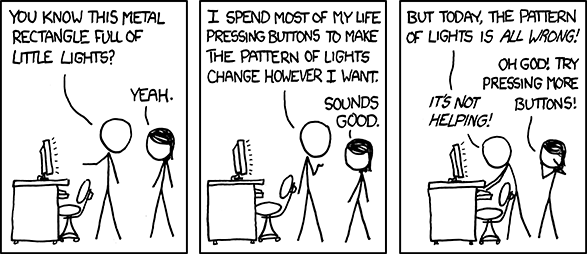
\includegraphics[width=1\textwidth]{introduction/figures/xkcd722(CC_BY-NC_2_5).png}
    xkcd.com/722 - CC BY-NC 2.5
\end{center}
\vfill

\allcontents
 %Exclude subsbubsections? Keep subsections?
\newpage

%\chapter*{Specific chapter contributions and acknowledgements}
\addcontentsline{toc}{chapter}{Additional informations for each specific chapters}

\section*{Contributions}
For each chapters, I designed the experiments, ran the analysis, interpreted the results and wrote the manuscripts. Natalie Cooper helped for designing the experiment and writing the manuscript.

\section*{Data availability and reproducibility}
\subsection*{Effects of missing data on topological inference using a Total Evidence approach}
All the code used in this analysis is available on \href{https://github.com/TGuillerme/Total_Evidence_Method-Missing_data}{GitHub} (\href{https://github.com/TGuillerme/Total_Evidence_Method-Missing_data}{    
goo.gl/4djNUf}) with some information on how to use the various functions. Additionally all the simulated data is available on \href{http://figshare.com/articles/Effect_of_missing_data_on_topological_inference_using_a_total_evidence_approach/1306861}{FigShare} (dx.doi.org/10.6084/m9.figshare.1306861).

\subsection*{Missing data in living mammals}
All data and analysis code is available on GitHub (\url{https://github.com/TGuillerme/Missing_living_mammals}).

\subsection*{Cretaceous-Palaeogene extinction does not affect mammalian disparity}
Data will be available on Dryad or Figshare.
Code for reproducing the analysis is available on GitHub (\url{https://github.com/TGuillerme/SpatioTemporal_Disparity}).


\section*{Specific chapters acknowledgements}
\subsection*{Effects of missing data on topological inference using a Total Evidence approach}
Thanks to Gavin Thomas, Fr\'{e}d\'{e}ric Delsuc, Emmanuel Douzery, Trevor Hodkinson, Andrew Jackson, Nick Matzke, and April Wright for useful comments on our simulation protocol and manuscript. Thanks to Paddy Doyle, Graziano D'Innocenzo and Sean McGrath for assistance with the computer cluster. Thanks to the two anonymous reviewers for their useful and enthusiastic comments.

\subsection*{Missing data in living mammals}
Thanks to David Bapst, Graeme Lloyd, Nick Matzke and April Wright.

\subsection*{Cretaceous-Palaeogene extinction does not affect mammalian disparity}
Thanks to Graeme Lloyd, Andrew Jackson, Gavin Thomas and Sive Finlay.



% \section*{Effects of missing data on topological inference using a Total Evidence approach}
% \subsection*{Data availability and reproducibility}
% All the code used in this analysis is available on \href{https://github.com/TGuillerme/Total_Evidence_Method-Missing_data}{GitHub} (\href{https://github.com/TGuillerme/Total_Evidence_Method-Missing_data}{    
% goo.gl/4djNUf}) with some information on how to use the various functions. Additionally all the simulated data is available on \href{http://figshare.com/articles/Effect_of_missing_data_on_topological_inference_using_a_total_evidence_approach/1306861}{FigShare} (dx.doi.org/10.6084/m9.figshare.1306861).
% \subsection*{Acknowledgements}
% Thanks to Gavin Thomas, Fr\'{e}d\'{e}ric Delsuc, Emmanuel Douzery, Trevor Hodkinson, Andrew Jackson, Nick Matzke, and April Wright for useful comments on our simulation protocol and manuscript. Thanks to Paddy Doyle, Graziano D'Innocenzo and Sean McGrath for assistance with the computer cluster. Thanks to the two anonymous reviewers for their useful and enthusiastic comments.

% \section*{Missing data in living mammals}
% \subsection*{Data availability and reproducibility}
% All data and analysis code is available on GitHub (\url{https://github.com/TGuillerme/Missing_living_mammals}).
% \subsection*{Acknowledgements}
% Thanks to David Bapst, Graeme Lloyd, Nick Matzke and April Wright.

% \section*{Cretaceous-Palaeogene extinction does not affect mammalian disparity}
% \subsection*{Data availability and reproducibility}
% Data will be available on Dryad or Figshare.
% Code for reproducing the analysis is available on GitHub (\url{https://github.com/TGuillerme/SpatioTemporal_Disparity}).
% \subsection*{Acknowledgements}
% Thanks to Graeme Lloyd, Andrew Jackson, Gavin Thomas and Sive Finlay.% TG: Two options, either all the details for chapters (i.e. who did what, code, acknowledgements) are written in is section, either they are as footnotes for each chapter (Natalie's thesis style)

\chapter*{Data availability and reproducibility}
\section*{Total Evidence and missing data}
All the code used in this analysis is available on GitHub (\url{https://github.com/TGuillerme/Total_Evidence_Method-Missing_data}) with some information on how to use the various functions. Additionally all the simulated data is available on Figshare (\url{http://dx.doi.org/10.6084/m9.figshare.1306861}).

\section*{Missing data in living mammals}
All data and analysis code is available on GitHub (\url{https://github.com/TGuillerme/Missing_living_mammals}).

\section*{Spatio-Temporal disparity in mammals at the K-Pg boundary}
Data is available on Figshare (\url{http://dx.doi.org/10.6084/m9.figshare.1539545}).
Code for reproducing the analysis is available on GitHub (\href{https://github.com/TGuillerme/SpatioTemporal_Disparity}{\url{https://github.com/TGuillerme/}}

\noindent\href{https://github.com/TGuillerme/SpatioTemporal_Disparity}{\url{SpatioTemporal_Disparity}}).

\newpage

\mainbody

\chapter{Introduction}
\label{chap:introduction}

%Some quote from GG Simpson
%"Certainly paleontologists have found samples of an extremely small fraction, only, of the earth's extinct species, and even for groups that are most readily preserved and found as fossils they can never expect to find more than a fraction.""
%But I'm not sure, maybe not quote is better.


%---------------------
%
% GENERAL INTRO - MAKE IT SHORT
% 
%---------------------

% Why is all this important? Dig from Benton and Fritz et al
The amazing diversity of organisms living on the biosphere represents an overwhelmingly low fraction of the organisms that ever existed \citep{novacek1992ext,raup1993extinction}, yet, most of the work in biology focus solely on living species \citep{fritzdiversity2013}.
Ignoring this, can lead to misinterpretation of macroevolutionary or macroecological patterns \citep{jacksonwhat2006,quentaldiversity2010,dietlconservation2011,slaterunifying2013,fritzdiversity2013,benton2015}.


Although most species that have ever lived are now extinct \citep{novacek1992ext,raup1993extinction}, the majority of macroevolutionary studies focus solely on living species (e.g. \citealp{meredithimpacts2011,jetzthe2012})


% Natalie: Interspecific competition is the negative effect one species has upon another by consuming, or controlling access to, a resource that is limited in availability (Keddy 1989).

Studying events in the evolutionary history of a taxonomic group, such as adaptive radiation or extinction, requires a fine-­‐scale and accurate resolution of their phylogenetic relationships through time. To achieve this, most scientists would agree that information about both extant and extinct species is needed. However, few efforts have been made to combine extant and extinct species in the same phylogenetic trees; instead phylogenetic trees usually contain only extant species. Because the vast majority of species in a lineage will be represented by extinct species, studies focusing on extant species contain less than 0.1\% of the lineage’s species richness. In some clades, ignoring extinct species may also obscure the true evolutionary history, species richness (i.e. Proboscidea), biogeography (i.e. Tinamiforms) or ecological diversity (i.e. Crocodilomorphs). Thus including the fossil record in these kinds of studies is essential to fully understand the evolutionary history of lineages.

In some clades, ignoring extinct species may also obscure the true evolutionary history or diversity of a clade. For example, in mammals the orders Perissodactyla (horses, rhinos and tapirs) and Proboscidea (elephants and mammoths) currently contain only a few taxa although they contained many more species in the past (Cifelli 1981, Antoine et al. 2003, Mihlbachler 2008, Seiffert et al. 2012). Crocodilomorph reptiles also had much greater species diversity (there were ~45 genera during the Paleogene1 but only nine today - Martin 2009) and larger geographic ranges (e.g. extinct Crocodilomorpha remains are found in northern France - Hua 1997) in the past. Finally, ignoring extinct diversity can lead to misinterpretation in comparative phylogenetic studies. For example, ignoring extinct Dinornithiforms (Moas) leads to misinterpretation of both the diversification pattern and biogeography of ratites (Jetz et al. 2012). Thus including the fossil record in these kinds of studies is essential to fully understand the evolutionary history of lineages (Slater et al. 2012).

% Add crocs et al example from steering committees reports

%(Maybe add a figure showing the real evolutionary history (a tree  with data) and what we actually know of it (a tree with a lot of data at the top)

% Bits
% Although most species that have ever lived are now extinct \citep{novacek1992ext,raup1993extinction}, the many large-scale macroevolutionary studies focus solely on living species (e.g. \citealp{meredithimpacts2011,jetzthe2012}).
% Throughout history, life on Earth has suffered a series of mass extinction events resulting in drastic declines in global biodiversity \citep[e.g.][]{RaupPT,BentonPT,rennetime2013,Brusatte2015}.
% There is an increasing consensus among evolutionary biologists that studying both living and fossil taxa is essential for fully understanding macroevolutionary patterns and processes \cite{slaterunifying2013,fritzdiversity2013,Wood01032013}.

% Ignoring fossil taxa may lead to misinterpretation of macroevolutionary patterns and processes such as the timing of diversification events \citep[e.g.][]{pyrondivergence2011}, relationships among lineages \citep[e.g.][]{manosphylogeny2007} or niche occupancy \citep[e.g.][]{pearmanniche2008}.
% For example, including both living and fossil taxa in evolutionary studies can improve the accuracy of timing diversification events (e.g. \cite{ronquista2012}, our understanding of relationships among lineages (e.g. \cite{beckancient2014}, and our ability to infer biogeographical patterns through time (e.g. \cite{Meseguer01032015}.
% However, the long-term effects of mass extinctions are more varied \citep{Erwin1998344}, and include increases in species richness in some clades \citep{friedmanexplosive2010}, species richness declines in others \citep{Benton85}, changes in morphological diversity \citep{Ciampaglio2001,Ciampaglio2004,kornextinction2013} and shifts in ecological dominance \citep[e.g.][]{Brusatte12092008,toljagictriassic-jurassic2013,bensonfaunal2014}.

% This has led to increasing consensus among evolutionary biologists that fossil taxa should be included in macroevolutionary studies \citep{jacksonwhat2006,quentaldiversity2010,dietlconservation2011,slaterunifying2013,fritzdiversity2013}.
% To do this, however, we need to be able to place living and fossil taxa into the same phylogenies; a task that remains difficult despite recent methodological developments \citep[e.g.][]{pyrondivergence2011,ronquista2012,BEASTmaster}.
% To perform such analyses it is necessary to combine living and fossil taxa in phylogenetic trees.
% One increasingly popular method, the Total Evidence method \cite{eernissetaxonomic1993,ronquista2012}, combines molecular data from living taxa and morphological data from both living and fossil taxa in a supermatrix (e.g. \cite{pyrondivergence2011,ronquista2012,schragocombining2013,slaterunifying2013,beckancient2014,Meseguer01032015}, producing a phylogeny with living and fossil taxa at the tips. 
% These shifts are characterized by the decline of one clade that is replaced by a different unrelated clade with a similar ecological role (e.g. Brachiopoda and Bivalvia at the end Permian extinction \citealt{Sepkiski1981,CLAPHAM01102006} but see \citealt{Payne22052014}). 

% These phylogenies can be dated using methods such as tip-dating \cite{ronquista2012,Wood01032013} and incorporated into macroevolutionary studies (e.g. \cite{ronquista2012,Wood01032013,slaterphylogenetic2013}.
% Shifts in ecological dominance are of particular interest because they are a fairly common pattern observed in the fossil record (e.g. Foraminifera; \citealt{D'Hondt01011996,Coxall01042006}; Ichtyosauria; \citealt{thorneresetting2011}; Plesiosauria; \citealt{bensonfaunal2014}) and are often linked to major macroevolutionary processes such as adaptive \citep{Losos2010} or competitive radiations \citep{Brusatte12092008}.

\section{Combining data, methods and disciplines}

%§ 2 - How can we combine them
%How can we combine them. Traditional approach down up (morphology) but modern approach top down (molecules)
The traditional way to combine both living and fossils data is using morphological data for both and draw conclusions on want happened.
However the problem is that such approach simply exclude living species (e.g. trilobites) or use living species just as a way to branch the fossil species in a macroevolutionary context (e.g. O'Leary or any other big cladistic paper?).
Also, the methods use to describe relations can be have big artefacts (e.g. parsimony) or other approaches (Mk) model can be oversimplistic (but still usuable).
Finally the data for fossils is usually restricted to morphology and the few ecological traits that can be extract from that (e.g. diet from teeth but not behaviour or population size)
Another approach for looking at macroevolution is to solely use living species (e.g. Jetz) one can look at the differences between DNA (many differences, good) and use models that are more realistic than Mk because of only four states(e.g. GTR).
Also this method can include time by calibrating the molecular clocks using fossils (Zuckerkandl).
However, appart from the use of the fossils occurence dates for making the clock tick, this approach ignores all clades that have no living descendant (the majority of clades!) and can even poorlierly estimate things from fossils.

Therefore, combining both data allows use to palliate to some of the problems of both approaches!


%§ 3 - What can we do when we combine them?
%Interesting studies or examples?

%§ 4 - In this thesis I worked on both aspects: how to combine them (TEM + missing mammals) and what to do with them (STD)

\section{Phylogenies with living and fossil species}

TEM Intro on the data story.

\subsection{Chapter 2: Effects of missing data on topological inference using a Total Evidence approach}

%§ 5 -Introducing chapter 1
%TEM and missing data (link missing data)
In the first chapter, I run long term and thorough simulation to test how robust are our phylogenetic inferences when we combine living taxa with molecular and morphological to fossil taxa with morphological data only.
I particularly focused on how missing data in both living and fossil taxa can affect topology.
I found that the number of living taxa with available data is essential to recover accurate topologies.
Therefore we need data for living mammals, how much of it is out there?
(This chapter is currently in review in Molecular Phylogenetics and Evolution - revisions).

\subsection{Chapter 3: Morphological data availability in living mammals}
%§ 6 -%ntroducing chapter 2
%(link missing data) Missing data in mammals (link mammals)
Following these results, I was interested in showing practical implications of this effect and monitored the morphological data availability for living mammals.
I downloaded all the recent available morphological matrices and counted the number of living mammals with available morphological data.
I then tested how these taxa where distributed accross the phylogeny to check if there weren't clustered in some specific clades.
I found that a lot of data is missing but that at least most of it is randomly distributed and should not drastically effect topology.
So it's not so bad, but what can we do with these total evidence trees?
(This chapter is an invited submission to a special issue in Biology Letters. Submission is due in December 2015).

\section{Total evidence phylogenies applications}

Once we have these trees we can do loads of cool stuff (primates ideas).

\subsection{Chapter 4: Cretaceous-Palaeogene extinction does not affect mammalian disparity}

% Cheesy quote for that bit "The most erroneous stories are those we think we know best - and therefore never scrutinize or question." Gould whenever

%§ 7 -Introducing chapter 3
%(link mammals) STD with mammals (link to cool stuff)
One important step in explaining macroevolutionnary processes is to accurately describe the patterns.
For example, to explain the processes driving diversification or extinction during a mass extinction event, we need to accurately measure what's happening.
One classical example is the K-T extinction where the effects still remain unclear after so many years of research.
Because I showed in the previous chapters that mammals are ok for combinations, I studied how they get affected by K-T disparity wise (INTRODUCE DISPARITY FIRST).
I found that...
All the cool stuff we can do with TEM!
(This chapter will be submitted to Evolution).

\section{Further applications} % TG: I think if the title stays as shitty, no need for a title.

%§ 8 - Introducing discussion
%(link to cool stuff) end.
Finally I will discuss all these cool stuff and how research might develop by doing the combinations of data and looking at more accurate descriptors of patterns (e.g. diversity AND disparity) blalbalblabla.
%Add the bits of discussion from TEM new conclusion

%§ 9 - Additional work % TG: or that bit can go in the conclusion?
In addition I was also interested in a side project on developing tools for phylogenetic correction that takes into account tree uncertainty.
I participated to a collaborative project exploring drivers of longevity accross birds and mammals led by Kevin Healy.
I developed the implementation to take tree uncertainty into account and this is now an available R pckage (mulTree).
%In addition to that I also did longevity.
%I was involved in developing the method and running the analysis for this paper. Phylogenetic correction is one crucial aspect in accurately describing maco patterns. In the paper, along with the main author, we developed and implemented a method for allowing to include phylogenetic uncertainty in generalized linear mixed models.

\bibliography{References} 



%---------------------------------------------
%
%       START
%
%---------------------------------------------

\chapter[Total Evidence method and missing data]{Total Evidence method and missing data}
\label{chap:TEM_paper}

\bigskip
\medskip
\begin{center}

\noindent{\Large \bf Effects of missing data on topological inference using a Total Evidence approach}
\footnote{A similar version of this chapter is currently (2015/09/30) in press as: "Thomas Guillerme, Natalie Cooper. in press. Effects of missing data on topological inference using a Total Evidence approach. \textbf{Molecular Phylogenetics and Evolution}; doi: \href{http://www.sciencedirect.com/science/article/pii/S1055790315002547}{doi:10.1016/j.ympev.2015.08.023}".}\footnote{\textit{Author contributions}: I designed the study, ran the analyses and wrote the paper. NC helped design the study and commented on drafts of the manuscript.}\\

\end{center}

%---------------------------------------------
%
%       ABSTRACT
%
%---------------------------------------------

% Illustration for TEM and Missing living data chapters (2 and 3)
\begin{figure}[h]
  \centering
  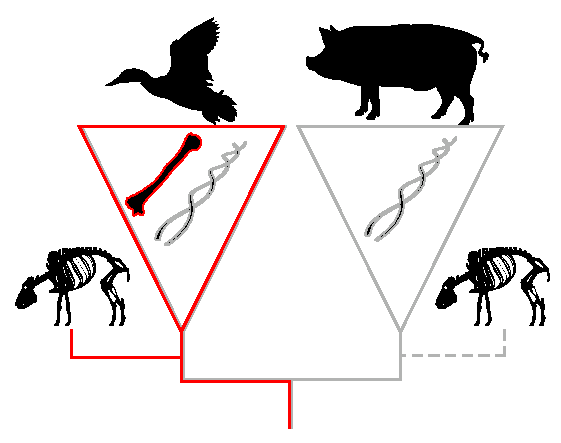
\includegraphics[width=\textwidth]{TEM/Figures/MissingDataFigure.pdf}
  \caption*{Fossil species can only branch with living ones that have morphological data available.}
\end{figure}

\newpage

\section*{Abstract}
To fully understand macroevolutionary patterns and processes, we need to include both extant and extinct species in our models.
This requires phylogenetic trees with both living and fossil taxa at the tips.
One way to infer such phylogenies is the Total Evidence approach which uses molecular data from living taxa and morphological data from living and fossil taxa.

Although the Total Evidence approach is very promising, it requires a great deal of data that can be hard to collect.
Therefore this method is likely to suffer from missing data issues that may affect its ability to infer correct phylogenies.

Here we use simulations to assess the effects of missing data on tree topologies inferred from Total Evidence matrices.
We investigate three major factors that directly affect the completeness and the size of the morphological part of the matrix: the proportion of living taxa with no morphological data, the amount of missing data in the fossil record, and the overall number of morphological characters in the matrix.
We infer phylogenies from complete matrices and from matrices with various amounts of missing data, and then compare missing data topologies to the ``best'' tree topology inferred using the complete matrix.

We find that the number of living taxa with morphological characters and the overall number of morphological characters in the matrix, are more important than the amount of missing data in the fossil record for recovering the ``best'' tree topology.
Therefore, we suggest that sampling effort should be focused on morphological data collection for living species to increase the accuracy of topological inference in a Total Evidence framework.
Additionally, we find that Bayesian methods consistently outperform other tree inference methods.
We therefore recommend using Bayesian consensus trees to fix the tree topology prior to further analyses.

\bigskip
\noindent
\textbf{Keywords:} morphological characters, Bayesian, Maximum Likelihood, topology, fossil, living.

%---------------------------------------------
%
%       INTRODUCTION
%
%---------------------------------------------

\newpage
\section{Introduction}
Although most species that have ever lived are now extinct \citep{novacek1992ext,raup1993extinction}, many large-scale macroevolutionary studies focus solely on living species (e.g. \citealp{meredithimpacts2011,jetzthe2012}).
Ignoring fossil taxa may lead to misinterpretation of macroevolutionary patterns and processes such as the timing of diversification events \citep[e.g.][]{pyrondivergence2011}, relationships among lineages \citep[e.g.][]{manosphylogeny2007} or niche occupancy \citep[e.g.][]{pearmanniche2008}.
This has led to increasing consensus among evolutionary biologists that fossil taxa should be included in macroevolutionary studies \citep{jacksonwhat2006,quentaldiversity2010,dietlconservation2011,slaterunifying2013,fritzdiversity2013}.
To do this, however, we need to be able to place living and fossil taxa into the same phylogenies; a task that remains difficult despite recent methodological developments \citep[e.g.][]{pyrondivergence2011,ronquista2012,BEASTmaster}.

Up to now, three main approaches have been used to place both living and fossil taxa into phylogenies.
These approaches differ mainly in how they treat fossil taxa and their data.
One can use fossils as tips or as nodes in the phylogeny, and can use only the age of the fossils, only the morphology of the fossils, or age and morphology jointly.
Classical cladistic methods use matrices containing morphological data from both living and fossil taxa and treat each taxon as a tip in the phylogeny. Relationships among the taxa are then inferred using optimality criteria such as maximum parsimony \citep{Hennig1966,felsenstein2004}.
This approach is commonly used by paleontologists but it ignores the additional molecular data available from living species and does not allow use of probabilistic methods for dealing with phylogenetic uncertainty.
Neontologists, on the other hand, more commonly use probabilistic approaches (e.g. Maximum Likelihood or Bayesian methods) based on matrices containing only molecular data from living species.
Because fossil taxa do not usually have available DNA, only fossil occurrence dates are used to time calibrate phylogenies \citep{zuckerkandl1965}.
There have been great improvements in the theory and application of these two approaches \citep[e.g.][]{bapsta2013,stadlerdating2013,heaththe2013} as well as much debate about the ``best'' approach to use \citep[e.g.][]{spencerefficacy2013,wrightbayesian2014}.
Neither approach, however, uses all the available data.

A final approach, known as the Total Evidence method, uses matrices containing molecular data from living taxa and morphological data from both living and fossil taxa \citep{eernissetaxonomic1993}.
This approach treats every taxon as a tip in the phylogeny, uses the occurrence age of the fossils to time calibrate the phylogeny \citep[known as tip-dating;][]{ronquista2012}, and allows the use of probabilistic methods for estimating phylogenetic uncertainty \citep{ronquista2012}.
The Total Evidence method is becoming an increasingly popular way of adding fossil taxa to phylogenies \citep[e.g.][]{pyrondivergence2011,ronquista2012,schragocombining2013,Slater2012MEE,beckancient2014,Arcila2015131}.
Although the Total Evidence approach seems very promising, there is one big drawback in using this approach: it requires both molecular and morphological data, both of which can be difficult (or impossible) to collect for every living and fossil taxon in the tree.
Morphological data for living taxa are rarely collected when molecular data are available (e.g. \citealp{O'Leary08022013} \textit{vs.} \citealp{meredithimpacts2011}), and for fossil taxa, data can only be collected from features preserved in the fossil record.
For example, in vertebrates, the hardest parts of the skeleton are more often preserved than soft parts \citep{sansomfossilization2013}; and molecular data are (nearly) always unavailable.
Therefore Total Evidence matrices are likely to contain a large proportion of missing data that may affect the method's ability to infer correct topologies, branch lengths and support values \citep{salamin2003}. 

Although missing data do not appear be a major problem in molecular and morphological matrices separately \citep[as long as enough data overlap in each case, and missing data are not phylogenetically biased;][]{wiensmissing2003,Wiens01102005,wiensmissing2006,wiensmissing2008,lemmonthe2009,Sanderson22072011,rouresite-specific2011,pattinsonphylogeny2014}, it may become more of an issue in Total Evidence matrices containing both molecular and morphological data for living and fossil taxa.
This may be particularly problematic as fossil taxa (generally) do not have molecular data, resulting in a large section of missing data in Total Evidence matrices.
Until now, few attempts have been made to study the impact of this missing data issue on phylogenetic inference in a Total Evidence framework \citep[i.e. using both molecular and morphological data;][]{Wiens01102005,manosphylogeny2007,pattinsonphylogeny2014}.
These previous studies assessed the effect of missing data on topology by either (1) comparing a dataset with missing data to subsets without missing data \citep{Wiens01102005}; or (2) removing both molecular and some morphological data from living taxa to create artificial fossils \citep{manosphylogeny2007,pattinsonphylogeny2014}.
Both approaches have shown that missing data are not a major problem and should not be an obstacle to combining both living and fossil species in the same phylogenies.
The way these studies were conducted, however, means that their conclusions are not generally applicable across all scenarios involving missing data in Total Evidence phylogenies.
For example, using an empirical (rather than simulation based) approach limits their conclusions to studies with similar distributions of data across species in the phylogeny.
Additionally, one of the three previous studies did not include fossil taxa in their analyses, so their results cannot be used to make conclusions about how missing data may influence the placement of fossils \citep{wiensmissing2003}. The other two studies did include fossil taxa, but used the patchiness of the fossil record to determine how to remove data from their matrices \citep{manosphylogeny2007,pattinsonphylogeny2014}. Data for living species are unlikely to be missing in this patchy way, instead full molecular data with the complete absence of morphological data is a likely pattern \citep{GuillermeCooperMissing}.
Finally, these previous studies mainly focused on how missing data in fossil taxa affect the placement of fossils, ignoring the effects of missing data in living species \citep{manosphylogeny2007,pattinsonphylogeny2014}.

In this study, we propose a theoretical assessment of the effect of missing data in the Total Evidence method by removing living taxa with morphological data, fossil data, all data for certain characters and the combination of these three aspects.
This is an advance on previous studies because we use large-scale simulations and analyse the effects of three distinct aspects of missing data thus focusing on both neontological and paleontological parts of the matrix.
In addition, we test the effect of missing data by measuring two crucial aspects of topology in both Maximum Likelihood and Bayesian phylogenies: (i) the conservation of clades \citep[based on the Robinson-Foulds distance;][]{RF1981} and (ii) the displacement of wild-card taxa \citep[based on the Triplets distance;][]{critchlowthe1996} rather than just a single measure of clade conservation or clade support \citep[cf.][]{Wiens01102005,pattinsonphylogeny2014}.

We focus on the effects of missing data on our ability to recover tree topology because it is a crucial aspect of a phylogeny in many macroevolutionary studies, for example when trying to elucidate the evolutionary relationships among species \citep[e.g.][]{meredithimpacts2011,jetzthe2012}, or for studying evolutionary transitions \citep[e.g.][]{friedmanexplosive2010}.
Although branch length estimation is also important \citep[namely for timing extinction and/or speciation events; e.g.][]{ronquista2012}, we do not consider branch lengths in this study.
This is partially due to difficulties with simulating branch lengths and topology simultaneously, but also because previous studies have already empirically assessed the effect of the Total Evidence method on branch length variation but using topological constraints \citep{ronquista2012,schragocombining2013,Slater2012MEE,beckancient2014}.
Thus understanding the sensitivity of topology to missing data is important for assessing the accuracy of tree estimation in the Total Evidence framework. To our knowledge, this question has never been formally assessed.

Here we use a simulation approach to assess the effect of missing data on tree topologies inferred from Total Evidence matrices.
Since the molecular part of a Total Evidence matrix acts like a ``classical" molecular matrix containing only the living taxa \citep{ronquista2012}, the effect of missing data on such matrices is well known \citep{wiensmissing2006,wiensmissing2008,lemmonthe2009,rouresite-specific2011}.
Therefore, we focus only on missing data in the morphological part of the matrix.
We investigate three major parameters that directly affect the completeness and size of the morphological part of the matrix, and reflect empirical biases in data availability: (i) the proportion of living taxa with no morphological data; (ii) the proportion of missing data in the fossil taxa; and (iii) the amount of morphological characters for both living and fossil taxa in the matrix (i.e. the size of the matrix).
We remove data from a Total Evidence matrix by changing the values of these three parameters and then assess how this affects the resulting tree topology.
We infer the topology from the matrices using both Maximum Likelihood and Bayesian inference methods and measure the differences in topology using two different topological distance metrics as proxies for clade conservation and for wild-card taxa placement.
We find that minimizing the number of living taxa with no morphological data and the number of missing morphological characters improves the ability of Total Evidence methods to recover the ``best'' tree topology more so than minimizing the amount of missing data in the fossil record.
Additionally, we find that the ability of Total Evidence methods to recover the ``best'' tree topology is increased when using Bayesian methods.



%---------------------------------------------
%
%       METHODS
%
%---------------------------------------------
 
\section{Materials and Methods}
To explore how missing data in the morphological partition of Total Evidence matrices influences tree topology, we used the following protocol (Fig. \ref{Fig_Outline}):
\begin{enumerate}
\item{Generating the matrix:} \label{step:generate_matrix} \\
We randomly generated a birth-death tree (hereafter called the ``true'' tree) and used it to simulate a matrix containing both molecular and morphological data for living and fossil taxa (hereafter called the ``complete'' matrix).
\item{Removing data:} \label{step:remove_data} \\
We removed data from the morphological part of the ``complete'' matrix to simulate the effects of missing data by modifying three parameters (i) the proportion of living taxa with no morphological data ($M_{L}$), (ii) the proportion of missing data in the fossil taxa ($M_{F}$) and (iii) the number of morphological characters ($N_{C}$). We call the resulting 125 matrices ``missing-data'' matrices.
\item{Estimating phylogenies:} \label{step:build_phylo} \\
We inferred phylogenetic trees from the ``complete'' matrix and from the 125 ``missing-data'' matrices resulting in one tree generated from a matrix with no missing data (hereafter called the ``best'' tree) and 125 trees inferred from the matrices with missing morphological data (hereafter called the ``missing-data'' trees). Phylogenies were inferred via both Maximum Likelihood and Bayesian approaches.
\item{Comparing topologies:} \label{step:compare_topo} \\
We compared the ``best'' tree to the ``missing-data'' trees to assess the influence of each parameter ($M_{L}$, $M_{F}$, $N_{C}$) and their interactions on the topologies of our phylogenies
\end{enumerate}
We repeated these four steps 50 times to account for variation in our random parameters in the simulations.

\begin{figure}[!htbp]
\centering
    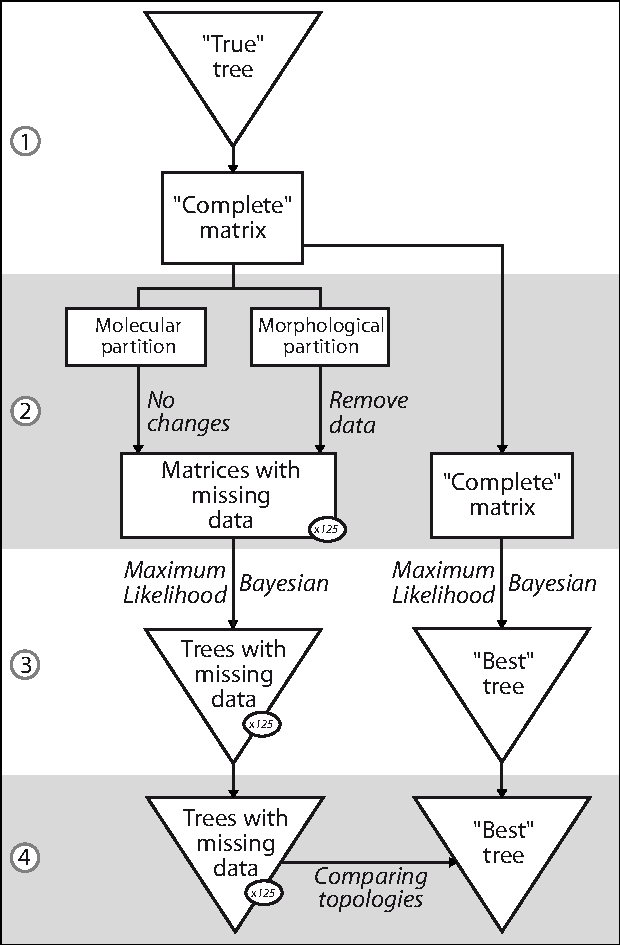
\includegraphics[width=0.8\textwidth]{TEM/Figures/Fig1.pdf}
\caption[Protocol outline]{\textbf{Protocol outline.}
(1) We randomly generated a birth-death tree (the ``true'' tree) and used it to simulate a matrix with no missing data (the ``complete'' matrix).
(2) We removed data from the morphological part of the ``complete'' matrix resulting in 125 ``missing-data'' matrices.
(3) We built phylogenetic trees from each matrix using both Maximum Likelihood and Bayesian methods.
(4) We compared the ``missing-data'' trees to the ``best'' tree.
We repeated these four steps 50 times.}
\label{Fig_Outline}
\end{figure}

%---------------------------------------------
%       1-Generating the matrix
%---------------------------------------------

\subsection{Generating the matrix}
\label{Generating_the_matrix}
First we randomly generated a ``true'' tree of 50 taxa in R v. 3.0.2 \citep{R} using the package diversitree v. 0.9-6 \citep{fitzjohndiversitree2012}.
We generated the tree using a birth death process by sampling speciation ($\lambda$) and extinction ($\mu$) rates from a uniform distribution (bounded between 0 and 1) but maintaining $\lambda$ $>$ $\mu$ \citep{paradistime-dependent2011}.
Empirical Total Evidence matrices vary in whether they have more fossil than living taxa or vice versa.
For example, fossil taxa make up 88\% \citep{beckancient2014}, 58\% \citep{schragocombining2013}, 48\% \citep{pyrondivergence2011}, 31\% \citep{ronquista2012} and 31\% \citep{Slater2012MEE} of taxa in various studies.
To avoid biasing our simulations towards either living or fossil taxa and to make each simulation comparable, we implemented a rejection sampling algorithm to select only trees with 25 living and 25 fossil taxa.
The fossil taxa were considered as unique tips at the end of extinct lineages.
We then added an outgroup to the tree, using the mean branch length of the tree to separate the outgroup from the rest of the taxa, and with the branch length leading to the outgroup set as the sum of the mean branch length and the longest root-to-tip length of the tree.

Next, we generated a molecular and a morphological matrix from the ``true'' tree.
The molecular matrix was simulated from the ``true'' tree using the R package phyclust v. 0.1-14 \citep{chen2011}.
The matrix contained 1000 character sites for 51 taxa and was generated using the seqgen algorithm \citep{ranbaut1997seqgen} and using the HKY model \citep{HKY85} with random base frequencies (sampled from a uniform probability distribution bounded between 0 and 1 with the total frequency for the four bases equal to 1) and transition/transversion rate of two \citep{douadycomparison2003}.
The substitution rates were selected from a gamma distribution with an ($\alpha$) shape of 0.5 \citep{yangamong-site1996}.
In practice, a value of $\alpha$ $<$ 1 decreases the number of sites with high substitution rates, thus reducing homoplasic sites and increasing the phylogenetic signal \citep{Hassanin1998611,EstoupHomoplasy}.
Also, we chose this $\alpha$ value to be consistent with our protocol for simulating morphological characters (see below).
This model and these parameter settings strike a balance between realism for empirical datasets \citep[e.g.][]{douadycomparison2003,kellymolecular2014} and parameter richness with more complex models (e.g., GTR, multiple partitions with independent models), making them more suitable for our computational limitations (even with the parameters defined, the total computational time for the whole analysis was around 150 CPU years).
All the molecular information for fossil taxa was replaced by missing data ("?").

We simulated the morphological matrix using the rTraitDisc function from the R package ape v. 3.0-11 \citep{paradisape:2004} to generate a matrix of 100 character sites for 51 taxa.
We assigned the number of character states (either two or three) for each morphological character by sampling with a probability of 0.85 for two states characters and 0.15 for three state characters.
We extracted these values from 100 random empirical matrices with more than 100 characters each downloaded from TreeBASE (\url{http://treebase.org/}).
We selected matrices published between 1985 and 2013 and covering 19 taxonomic classes (Chordata, Arthropoda, Annelida, Angiosperm, Gymnosperm and Pteridophyta).
These matrices contained a cumulative number of 22563 characters that had between two and 10 character states.
We then extracted the proportion of characters with each number of states (two to 10) to give us an empirical estimate of the average number of character states for each character, as shown in Fig. \ref{Fig_AppendixCharacters}.
Most morphological characters have two or three states, therefore we only simulate characters with two or three states, and sampled these in proportion to their occurrence in our empirical data (probability of 0.85 for two states characters and 0.15 for three state characters).

We then ran an independent discrete character simulation for each character using the ``true'' tree with the character's randomly selected number of states (two or three) and assuming an equal rate of change (i.e. evolutionary rate) from one character state to another \citep{Pagel22011994}.
This method allows us to have only two parameters for each character: the number of states and the evolutionary rate.
For each character, the evolutionary rate was sampled from a gamma distribution with $\alpha$ = 0.5.
We used low evolutionary rate parameters to be consistent with the molecular rate parameters, to avoid homoplasy in the morphological part of the matrix and create a clear phylogenetic signal \citep{wrightbayesian2014}.
Topological error has been shown to be minimal at a morphological rate of 0.5 when using the M\textit{kv} model \citep{lewisa2001,wrightbayesian2014}.
Note, however, that \cite{wrightbayesian2014} have shown that low morphological rates ($<$ 0.5) increase variance in topological error, but we discarded simulations with such topological error by selecting only matrices with a ``fair'' phylogenetic signal \citep[see Estimating phylogenies section below;][]{zanderminimal2004} so this should not influence our results.

\begin{figure}[!h]
\centering
    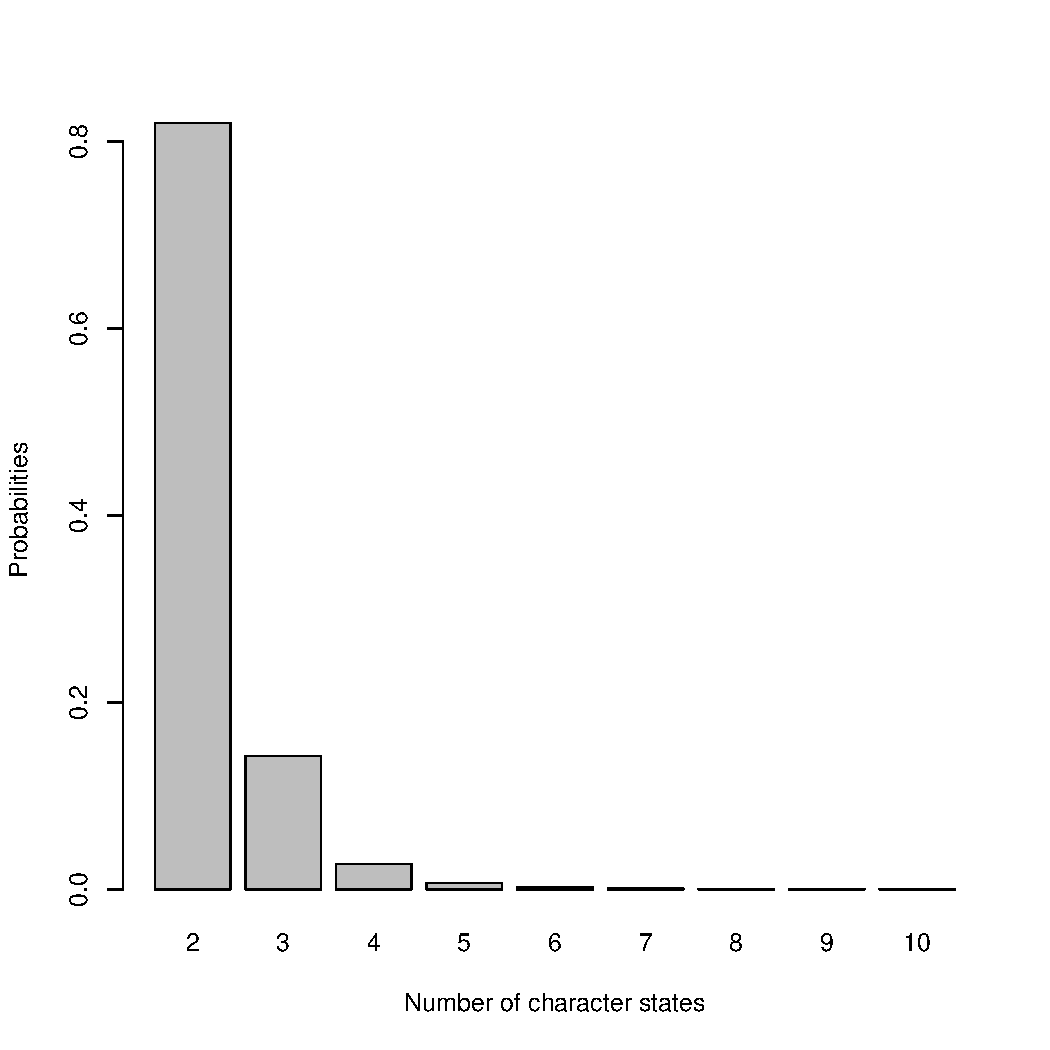
\includegraphics[keepaspectratio=true,width=0.8\textwidth]{TEM/Figures/TEM_Fig-AppendixCharacters.pdf}
\caption[Empirical proportion of morphological characters]{The proportion of morphological characters with between two and 10 character states extracted from 100 randomly selected empirical matrices downloaded from TreeBASE.}
\label{Fig_AppendixCharacters}
\end{figure}


Finally, we combined the morphological and molecular matrices obtained from the ``true'' tree.
Hereafter we call this the ``complete'' matrix, i.e. the matrix with no missing data except for the molecular data of the fossil taxa.

%---------------------------------------------
%       2-Removing data
%---------------------------------------------

\subsection{Removing data}
To explore the effect of missing morphological data on topological recovery, we removed various amounts of the ``complete'' matrix to obtain matrices with missing morphological data.
Hereafter, we call these matrices with missing morphological data the ``missing-data'' matrices.
Note that the amount of molecular data remained constant throughout our simulations: 1000 molecular characters for living taxa and no molecular data for fossil taxa (see above).
We removed morphological data using three data incompleteness parameters:
\begin{enumerate}
\item{The proportion of missing living taxa ($M_L$).}
This first missing-data parameter corresponds to the proportion of living taxa with no morphological data. It represents the number of living taxa that are present in the matrix but have only molecular data available. This reflects the fact that, because of the increasing ease of collecting molecular data, morphological data for living species are rarely collected \citep{GuillermeCooperMissing}.
Therefore, many living species will have only molecular data available.
In practice, we removed all the morphological data from randomly chosen living taxa with five different proportions: 0\%, 10\%, 25\%, 50\% or 75\% of living taxa with no morphological data.
\item{The proportion of missing data in the fossil record ($M_F$).}
This missing data parameter represents the completeness of the fossil record.
Due to preservation biases, missing data for fossil taxa are common \citep{sansomfossilization2013}.
In practice, we randomly removed a proportion of data from across the fossil taxa with five different proportions: 0\%, 10\%, 25\%, 50\% or 75\% of overall missing data for the fossil taxa.
Note that 50\% missing data for fossil taxa does not mean that each fossil is missing 50\% of its morphological data.
Instead this 50\% refers to missing fossil data across the whole matrix.
Some fossils may retain 100\% of their data and others may lose most of their data at this parameter value (down to a minimum threshold of 5\% available data; see below).
\item{The number of morphological characters for both living and fossil taxa ($N_C$).}
This parameter is not a missing data parameter \textit{per se} but rather an indication of the size of the matrix.
Any morphological matrix of any size has indeterminate missing data, given that the total number of characters is undefined, but presumably large.
Therefore, this parameter corresponds to the overall number of characters available for both living and fossil taxa.
In practice, we randomly removed entire characters from the morphological matrix reducing it to: 100, 90, 75, 50 or 25 characters.
Note that these levels are equivalent to the two other parameters (i.e. 0\%, 10\%, 25\%, 50\% or 75\% of ``missing'' morphological characters).
\end{enumerate}

Each parameter represents a different way of removing data from the morphological part of the matrix: $M_L$ removes entire rows from the living data; $M_F$ removes cells from the fossil data; and $N_C$ removes columns across both living and fossil data.
Note that $M_L$ and $M_F$ differ not only because of the region of the matrix affected: for $M_L$ all the morphological data of a percentage of living taxa are removed, whereas for $M_F$ a percentage of the data are removed at random from across the whole of the morphological matrix for fossil taxa.

We created matrices using all parameter combinations resulting in 125 ($5^3$) ``missing-data'' matrices.
Note that one of these combinations ($M_L$=0\%; $M_F$=0\% and $N_C$=100) has no missing data so is equivalent to the ``complete'' matrix, thus we have one effectively complete matrix in our 125 ``missing-data'' matrices.
In practice, we first removed the data following the two missing data parameters $M_L$ and $M_F$ and then removed data following the $N_C$ parameters.
To avoid avoid matrices containing taxa without any data (morphological or molecular), we repeated the random deletion until the matrices contained at least 5\% of data for any taxon.
Note that the living taxa always had at least 90\% of data (the 1000 molecular characters).

%---------------------------------------------
%       3-Building phylogenies
%---------------------------------------------

\subsection{Estimating phylogenies}
From the resulting matrices we generated two types of trees: the ``best'' tree inferred from the ``complete'' matrix and the ``missing-data'' trees inferred from the 125 matrices with various amounts of missing data.
The ``true'' tree was used to generate the ``complete'' matrix and reflects the ``true'' evolutionary history in our simulations.
The ``best'' tree, on the other hand, is the best tree we can build using state-of-the-art phylogenetic methods.
In real world situations, the ``true'' tree is never available to us because we cannot know the true evolutionary history of a clade \citep[except in very rare circumstances, e.g.][]{rozen2005}.
We compare ``best'' trees to ``missing data'' trees but could also compare ``true'' trees to the ``missing data'' trees.
In practice, the difference between the ``best'' trees and the ``missing data'' trees represents the effect of our missing data parameters and of the phylogenetic methods used to infer the ``missing data'' trees.
The difference between the ``true'' and the ``missing data'' trees, however, represents the effect of our parameters used to generate the ``true'' tree and the algorithms used to generate the ``complete'' matrix as well as the effect of our missing data parameters and the phylogenetic methods used.
Because the main aim of this study is to look at the effect our missing data parameters on topological recovery, we chose to represent only the comparisons between the ``best'' trees and ``missing data'' trees.
The results of the comparisons of the ``true'' tree and the ``missing data'' trees are available in Supplementary data A.1. %link?
Note that this makes little difference to our overall results.

\subsubsection*{Maximum Likelihood}
The ``best'' tree and the ``missing-data'' trees were inferred using RAxML v. 8.0.20 \citep{Stamatakis21012014}. For the molecular data, we used the GTR + $\Gamma_4$ model (\citealp{tavare1986}; default GTRGAMMA in RAxML v. 8.0.20; \citealp{Stamatakis21012014}).
For the morphological data, we used the M\textit{kv} model \citep{lewisa2001} assuming an equal state frequency and a unique overall substitution rate ($\mu$) following a gamma distribution of the rate variation with four distinct categories (M\textit{kv} + $\Gamma_4$; -K MK option in RAxML v. 8.0.20; \citealp{Stamatakis21012014}).
We used RAxML because it automatically corrects for acquisition bias \citep{lewisa2001}. It is also heavily used in the literature for Maximum Likelihood tree inference \citep[e.g.][]{rouresite-specific2011,Bogdanowicz2012,springermacroevolutionary2012,O'Leary08022013,kellymolecular2014} and is one of the fastest methods available \citep{Stamatakis01102008}. 

To measure the support for each branch in our simulated phylogenies we first ran a fast bootstrap analysis (Lazy Sub-tree Rearrangement) with 500 replicates on the ``complete'' matrix.
We removed all the simulations with a median bootstrap support lower than 50 as a proxy for weak phylogenetic signal \citep{zanderminimal2004}.
We repeated this selection until we obtained 50 sets of simulations (i.e. 50 ``complete'' and 50 x 125 ``missing-data'' matrices) with a relatively strong phylogenetic signal (median bootstrap $>$ 50).
This step was implemented to make sure that the differences we observed in topologies (see below) were due to the amount of missing data for each parameter ($M_L$, $M_F$ and $N_C$) and not simply to low branch support that is likely to lead to different topologies.
On these selected simulations, we used the fast bootstrap algorithm and performed 1000 bootstraps for each tree inference to assess topological support \citep{pattengale2010many}.
Using these parameters took \texttildelow 8 CPU years to build 50 sets of 125 bootstrapped Maximum Likelihood trees (2.30GHz clock speed nodes). We performed this procedure to increase the resolution of our resulting trees. 

\subsubsection*{Bayesian Inference}
The ``best'' tree and the ``missing-data'' trees were inferred using MrBayes v. 3.2.1 \citep{Ronquist2012mrbayes}.
We partitioned the data to treat the molecular part as a non-codon DNA partition and the morphological part as a multi-state morphological partition.
The molecular evolutionary history was inferred using the HKY model with a transition/transversion ratio of two \citep{douadycomparison2003} and a gamma distribution for the rate variation with four distinct categories (HKY + $\Gamma_4$).
For the morphological data, we used the M\textit{kv} model \citep{lewisa2001}, with equal state frequency and a unique overall substitution rate ($\mu$) with four distinct rates categories (M\textit{kv} + $\Gamma_4$).
Note that MrBayes automatically corrects for acquisition bias in the morphological data partition \citep{Nylander01022004,Ronquist2012mrbayes}.
We chose these models to be consistent with the parameters used to generate the ``complete'' matrix.

Each Bayesian tree was estimated using two runs of four chains each for a maximum of 5$\times$$10^7$ generations.
For each estimation, we used the ``true'' tree's topology as a starting tree (with a starting value for each branch length of one).
We used a fixed starting tree rather than a random starting tree \citep[default MrBayes;][]{Ronquist2012mrbayes} to speed up our Bayesian inferences.
To assess if this had an effect on the topology of the ``best'' tree, we ran a sub-sample of trees using a different random starting tree for the two MCMC chains \citep[default MrBayes option;][]{Ronquist2012mrbayes}.
We tested this effect on five trees with the five levels of missing data (i.e. first tree: $M_L$=0\%, $M_F$=0\% and $N_C$=100 (i.e. 0\% ``missing''); second tree: $M_L$=10\%, $M_F$=10\% and $N_C$=90, etc.) on the first 20 simulation chains.
We then compared the trees inferred using a random starting tree to the ``best'' tree using the normalised Robinson-Foulds and Triplets metrics in an identical way as described below (Fig. ~\ref{Fig_startingTree}).

\begin{figure}[!htbp]
\centering
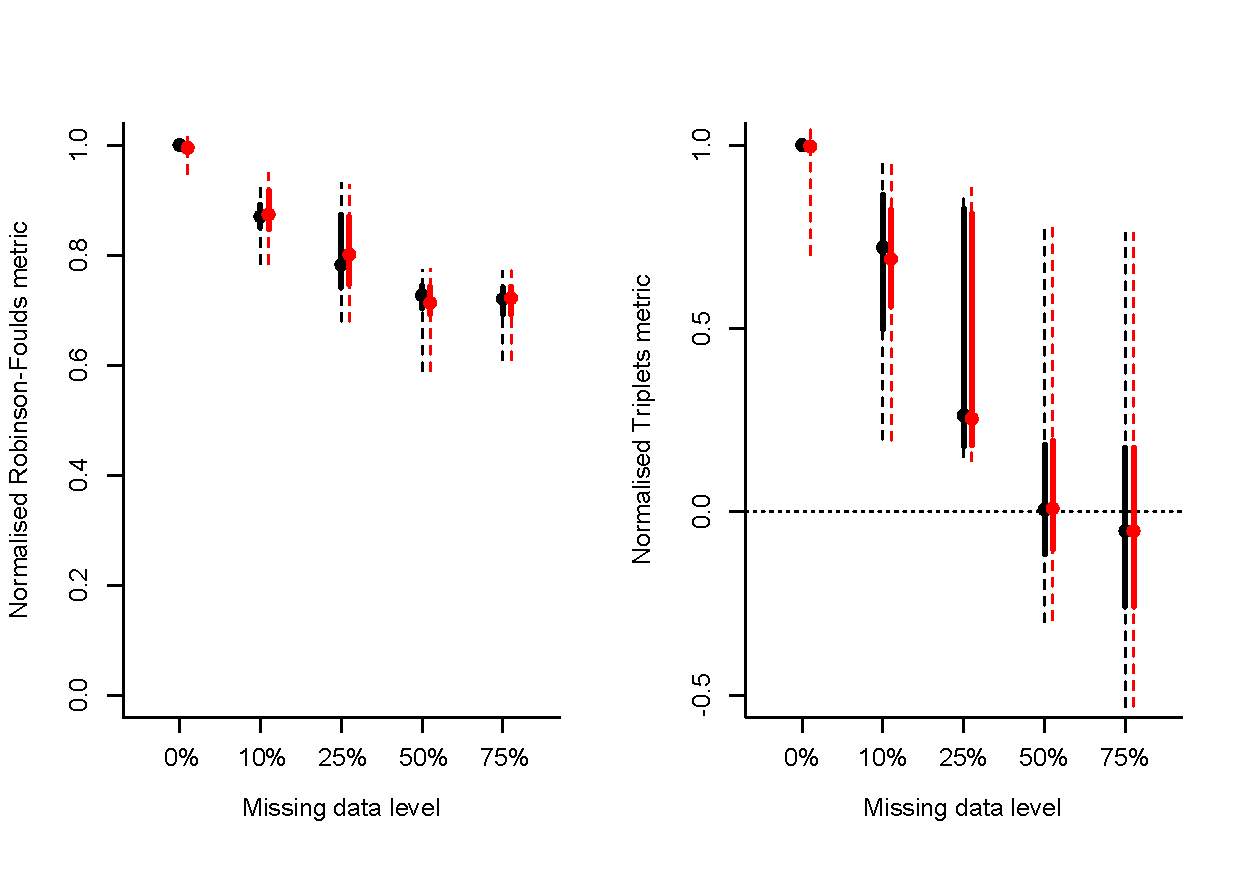
\includegraphics[keepaspectratio=true, width=\textwidth]{TEM/Figures/Starting_tree.pdf}
\caption[Effect of using the ``true'' tree as a starting tree]{Effect of using the ``true'' tree (black) or a random tree (red) as the starting tree for the Bayesian inference. The x axis, represents the amount of missing data (see below).}
\label{Fig_startingTree}
\end{figure}

We used a two-way ANOVA to test any significant effect of the starting tree (``true'' or random) on the normalised Robinson-Foulds and Triplets metrics.
We found no significant effect of using the ``true'' instead of a random tree as a starting tree on our ability to recover the ``best'' tree (Table ~\ref{Tab_lm_res}).
Note that these results are not surprising since a starting tree is not a Bayesian prior on topology \textit{per se}.

Additionally, we used two priors on the molecular part of the matrix: an exponential prior on the shape of the gamma distribution of $\alpha$ = 0.5, and a transition/transversion ratio prior of two sampled from a strong beta distribution ($\beta$(80,40)); and one prior on the morphological part of the matrix (exponential prior on the shape of the gamma distribution of $\alpha$ = 0.5).
We used these priors to speed up the Bayesian estimation process.
These priors biased the way the Bayesian process calculated branch lengths by giving non-random starting points and boundaries for parameter estimation however, here we are focusing on the effect of missing data on tree topology and not branch lengths.
Even using these priors, it took $~$ 140 CPU years to build 50 sets of 125 Bayesian trees (2.30GHz clock speed nodes).
The detailed MrBayes parameters are available in Supplementary data A.2. %link
We also included an analysis showing the effect of missing data on the estimation of the shape parameter ($\alpha$) of the morphological substitution rate distribution.
This extra analysis, however, is beyond the scope of this paper so the results are not discussed further here.

\begin{table}[ht]
\caption[Effect of using the ``true'' tree as a starting tree]{Test of the effect of using either a random tree or the ``true'' tree as a starting tree on two Normalised Robinson-Foulds (RF) and Triplets (Tr) metrics using a two-way ANOVA.}
\label{Tab_lm_res}
\centering
\begin{tabular}{rlcccccc}
  \hline
 metric & terms & Df & Sum Sq & Mean Sq & F value & Pr($>$F) \\ 
  \hline
RF & starting    & 1 & 0.00 & 0.00 & 0.01 & 0.9125 \\ 
   & Residuals   & 198 & 2.97 & 0.01 &  &  \\ 
Tr & starting    & 1 & 0.01 & 0.01 & 0.07 & 0.7887 \\ 
   & Residuals   & 198 & 34.57 & 0.17 &  &  \\ 
   \hline
\end{tabular}
\end{table}

We used the average standard deviation of split frequencies (ASDS) as a proxy to estimate the convergence of the chains and used a stop rule when the ASDS went below 0.01 \citep{Ronquist2012mrbayes}.
We also checked the effective sample size (ESS) on a random sub-sample of runs in each simulation to ensure that ESS $>>$ 200 \citep{drummond2006ess}.
Finally we built a strict majority rule Bayesian consensus tree from the combined chains, excluding the 25\% first iterations as burn-in \citep{Ronquist2012mrbayes}.

%---------------------------------------------
%       4. Comparing Topologies
%---------------------------------------------

\subsection{Comparing topologies}
We compared the topology of the ``missing-data'' trees to the ``best'' tree to measure the effect of the three parameters $M_{L}$, $M_{F}$ and $N_{C}$ on tree topology.
We used the Robinson-Foulds distance \citep{RF1981} to assess the number of conserved clade positions and the Triplets distance \citep{dobson1975triplets} to assess the number of wildcard taxa \citep[i.e. taxa that frequently change position in different trees][]{kearneyfragmentary2002}. We used these two metrics because they illustrate two different aspects of tree topology (see Discussion) but also because their performance in measuring differences in topology is well described \citep{Kuhner04112014} and well implemented \citep{Bogdanowicz2012}.
We normalised both metrics using methods described in \citet{Bogdanowicz2012} to generalize our results for any \textit{n} number of taxa.
These metrics are described in detail below.

\subsubsection*{Robinson-Foulds distance}
The Robinson-Foulds distance \citep{RF1981}, or ``path difference", measures the difference between the number of clades and twice the number of shared clades across two trees.
The metric reflects the distance between the distributions of tips among clades in the two trees \citep{RF1981}:
\begin{equation}
RF_{x,y} = N_{x} + N_{y} - 2C_{x,y}
\end{equation}
where $C_{x,y}$ is the number of clades in common in the two trees.
$C$ is equal to one if the two trees have the same $n$ taxa; and $C = n-2$ when none of the $n$ taxa are shared between the trees.
This metric is bounded between zero, when the two trees are identical, and $2(n-2)$ (for two trees with $n$ taxa) when there is no shared clade in the two trees.
This metric is sensitive to minor changes in clade conservation: if the trees are composed of two clades of three taxa \textit{(((a,b),c),((d,e),f))}, the swapping of any two taxa will lead to a maximal score of the Robinson-Foulds distance indicating poor tree similarity.

We normalised this metric following Bogdanowicz's Normalised Tree Similarity (NTS) method \citep{Bogdanowicz2012}.
For any tree with \textit{n} taxa compared using a tree difference metric $m$, Normalized Tree Similarity, $NTS_m$, represents the similarity score for the two trees given the expected difference between 1000 random Yule trees \citep{Bogdanowicz2012} with $n$ taxa. If $\bar{d}_{m,n}$\textit{(rand)} is the average difference between two random Yule trees with $n$ taxa and $d_{m,n}$\textit{(x,y)} the difference between the two trees \textit{x} and \textit{y} each containing $n$ taxa, then:
\begin{equation}
NTS_{m,n}(x,y)=\frac{\bar{d}_{m,n}(rand) - d_{m,n}(x,y)} {\bar{d}_{m,n}(rand)}
\end{equation}
\textit{NTS} ranges from one to -$\infty$.
For any $m,n$, when $NTS$ = 1, the trees are identical, when \textit{NTS} = 0 the trees are no more different than expected by chance, and when $NTS$ $<$ 0, the trees are more different than expected when comparing two random trees. 

This method is a generalisation of the topological accuracy method \citep{Price2010} allowing to compare topological differences between any tree with any tree comparison metric.
In practice when the Normalised Robinson-Foulds metric between two trees is equal to one, the trees are identical; if the metric is equal to zero, the trees are no more different than expected by chance; finally if the metric is less than zero, the trees are more different than expected by chance.
Note that once rescaled, the Normalised Robinson-Foulds metric is a measure of similarity, rather than of distance like the original Robinson-Foulds metric. 

\subsubsection*{Triplets distance}
The Triplets distance \citep{dobson1975triplets} measures the number of sub-trees made up of three taxa that differ between two trees \citep{critchlowthe1996}:
\begin{equation}
S_n = \sum_{ijk} I_{ijk}
\end{equation}
where:
\begin{equation}
\sum_{ijk} = \binom{n}{4} = \frac{n!}{4!(n-4)!}
\end{equation}
and where \textit{n} is the total number of taxa in both trees (modified from \cite{critchlowthe1996}).
If $S_n$ = 0, the trees are identical; when $S_n$ = $\binom{n}{4}$, the trees are as different as possible (i.e. every taxon has a different placement in the two trees).
This metric measures the position of each taxon and clade in relation to its closest neighbours.
It is bounded between zero when the two trees are identical and $\binom{n}{3}$ (for two trees with $n$ taxa) when there is no shared taxa/clade position in the two trees.
Therefore this metric is sensitive to the conservation of wildcard taxa.
We normalised this metric in the same way as for the Robinson-Foulds distance resulting in the Normalised Triplets metric.

\subsubsection*{Paired tree comparisons}
\label{tree_comparisons}
For the Maximum Likelihood and Bayesian consensus trees we performed pairwise comparisons between the ``best'' tree and each ``missing-data'' tree using both the Normalised Robinson-Foulds and Normalised Triplets metrics with the TreeCmp java script \citep{Bogdanowicz2012} resulting in 125 Normalised Robinson-Foulds metrics and 125 Normalised Triplets metric for each tree inference method.
Also, to take into account the uncertainty of tree inference, we extracted 1000 random bootstrapped trees from the Maximum Likelihood analysis and 1000 trees from the posterior tree distribution of the Bayesian analysis for the ``best'' trees, and then did the same for the 125 ``missing data" trees (resulting in 1000 ``best'' trees and 125$\times$1000 ``missing data" trees). 
For a given set of 1000 ``missing data" trees and the 1000 ``best'' trees, we sampled one ``missing data" tree and one ``best'' tree at random and compared them using both the Normalised Robinson-Foulds and Normalised Triplets metrics as described above.
We repeated this 1000 times for each set of ``missing data" trees resulting in 125$\times$1000 values for each metric.
We repeated all the paired tree comparisons described above for each of the 50 simulation runs.
We then calculated the mode and the 50\% and 95\% confidence intervals from the resulting distribution using the hdrcde R package v. 3.1 \citep{hdrcde}.

\subsection{Testing the effects of the missing data parameters on topological recovery}
Finally, we tested the effects of our missing data parameters ($M_{L}$, $M_{F}$, $N_{C}$ and their interactions) on our ability to recover the ``best'' tree topology in a Total Evidence framework.
We also assessed the effect of our missing data parameters jointly with the effects of different tree inference and uncertainty methods (i.e. Maximum Likelihood, Bayesian consensus, Maximum Likelihood bootstrap trees and Bayesian posterior tree distribution).

We measured similarities among the distributions of the different metrics scores (Normalised Robinson-Foulds and Normalised Triplets metric) using the Bhattacharyya Coefficient \citep{Bhattacharyya}.
The Bhattacharyya Coefficient is the probability of overlap between two distributions bounded between 0 (no overlap) and 1 \citep[full overlap;]{Bhattacharyya}.
The coefficient is calculated as the sum of the square root of the relative counts shared in \textit{n} bins among two distributions.
\begin{equation}
\text{Bhattacharyya Coefficient}=\sum_{i=1}^{n} \sqrt{{\sum{a_i}}\times{\sum{b_i}}}
\end{equation}
where
\begin{equation}
{a_i}=\frac{\text{Number of counts in bin \textit{i} for the distribution \textit{a}}}{\text{Total number of counts for the distribution \textit{a}}}
\end{equation}
and
\begin{equation}
{b_i}=\frac{\text{Number of counts in bin \textit{i} for the distribution \textit{b}}}{\text{Total number of counts for the distribution \textit{b}}}
\end{equation}
The precision of the Bhattacharyya Coefficient is directly related to the number of bins, $n$. If $n$ is low, the overlap will be overestimated and if $n$ is too high, the overlap will be underestimated. In this analysis, we determined the number of bins using Silverman's rule of thumb which states that $n$ should be 0.9 times the minimum of the standard deviation and the interquartile range of the distribution, divided by 1.34 times the sample size of the distribution to the negative one-fifth power (\texttt{bw.nrd0()} function in R \citep{silverman1986density}).
When the Bhattacharyya Coefficient between two distributions is $<$0.05, the distributions are significantly different.
When this coefficient is $>$0.95 both distributions are significantly similar.
Values in between these two threshold just show the probability of overlap between the distributions but are not conclusive to assess the similarity or differences between the distributions.

Note that this is comparable to performing a two-sided t-test, but we use the Bhattacharyya Coefficient here because we are comparing whole distributions not just their means.
When the Bhattacharyya Coefficient between two distributions is $<$0.05, the distributions are significantly different.
When this coefficient is $>$0.95, the distributions are significantly similar.
Values between these two thresholds show the probability of overlap between the distributions but do not allow us to define the significance of the similarity or differences between distributions.
To assess the effect of our missing data parameters, we calculated the Bhattacharyya Coefficient between the distributions of the different metrics scores (Normalised Robinson-Foulds and Normalised Triplets metric) for each pairwise combination of missing data parameters ($M_{L}$, $M_{F}$, $N_{C}$) and parameter states (0\%, 10\%, 25\%, 50\%, 75\% and 100, 90, 75, 50, 25 characters), i.e. $M_{L}$ = 0\%, $M_{F}$ = 0\%, $N_{C}$ = 100; $M_{L}$ = 10\%, $M_{F}$ = 0\%, $N_{C}$ = 100 etc. (see Fig. \ref{Fig_Bhattacharyya_Coefficients1} for more details).
This resulted in 7875 pairwise comparisons (a triangular matrix with $3^5$$\times$$3^5$ cells).
We performed this procedure separately for each tree inference and uncertainty method.
When two combinations of missing data parameters have a similar ability to recover the ``best'' tree topology the Bhattacharyya Coefficient will be close to one.
Conversely, if the two combinations of missing data parameters differ, the Bhattacharyya Coefficient will be close to zero.
Because of the difficulties in representing so many pairwise comparisons in a meaningful way, we summarized these results as a heat map of Bhattacharyya Coefficients (see Fig. \ref{Fig_Results-paircomp_within1} and \ref{Fig_Results-paircomp_within2}).
In this type of figure, parameters that have similar effects on recovering the ``best'' topology (either positive or negative effects) will be denoted by similar colour patches in the heat map representation of these comparisons (see Fig. \ref{Fig_Results-paircomp_within1} and \ref{Fig_Results-paircomp_within2}).

 \begin{figure}[!h]
 \centering
     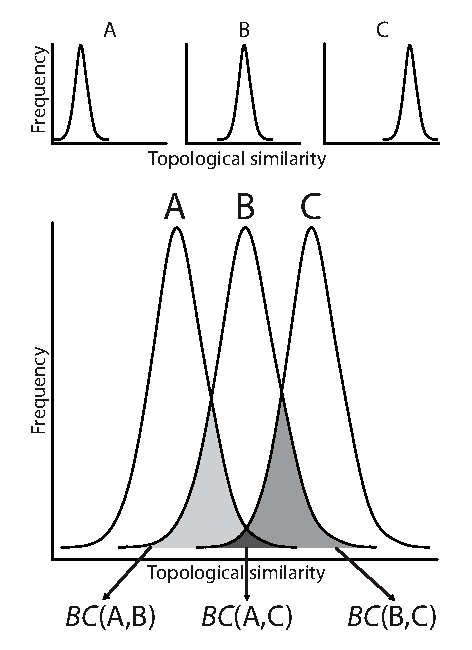
\includegraphics[width=0.5\textwidth]{TEM/Figures/Fig2.pdf}
 \caption[Bhattacharyya Coefficient calculation outline 1]{\textbf{Bhattacharyya Coefficient calculation outline 1.} A, B and C are distributions of tree similarity metrics (Normalised Robinson-Foulds or Normalised Triplets metrics) for any combination of missing data parameters (e.g. $M_{L}$ = 10\%, $M_{F}$ = 50\%, $N_{C}$ = 25). The Bhattacharyya Coefficient (BC) is the overlap of the distribution of tree similarity metrics between two combinations of missing data parameters, for example, BC(A,B) is the probability of overlap between the distributions A and B.}
 \label{Fig_Bhattacharyya_Coefficients1}
 \end{figure}

To assess the effect of the different tree inference and uncertainty methods (i.e. Maximum Likelihood, Bayesian consensus, Maximum Likelihood bootstrap trees and Bayesian posterior tree distribution) on our ability to recover the ``best'' tree topology, we calculated the Bhattacharyya Coefficient between the distributions of the different metrics scores (Normalised Robinson-Foulds and Normalised Triplets metric) for each pairwise combination of tree inference and uncertainty methods, i.e. Maximum Likelihood \textit{versus} Bayesian consensus; Maximum Likelihood \textit{versus} Maximum Likelihood bootstrap trees etc. (see Fig. \ref{Fig_Bhattacharyya_Coefficients2} for more details).
Note that this procedure pools results from across all missing data parameter combinations so it results in just six pairwise comparisons.
When two tree inference or uncertainty methods have a similar ability to recover the ``best'' tree topology the Bhattacharyya Coefficient will be close to one.
Conversely, if the two tree inference or uncertainty methods differ, the Bhattacharyya Coefficient will be close to zero.

\begin{figure}[!h]
\centering
    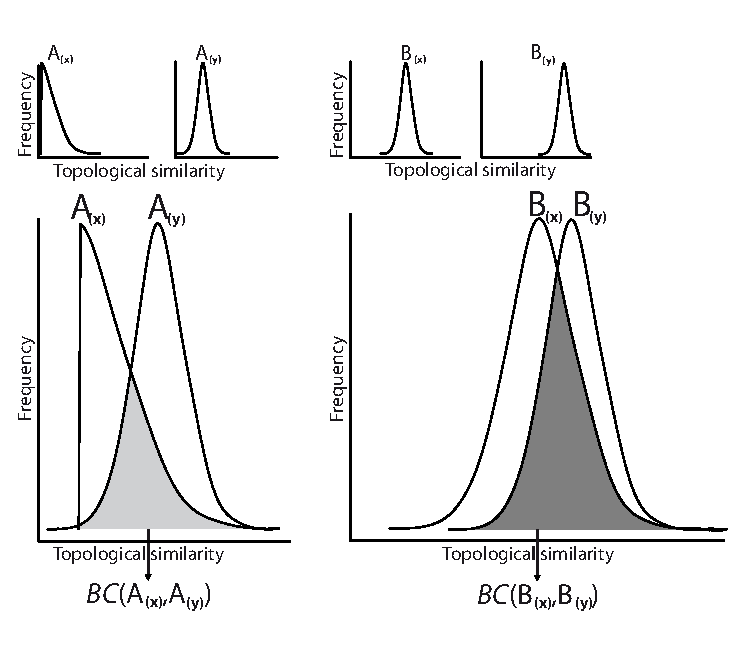
\includegraphics[width=1\textwidth]{TEM/Figures/Fig3.pdf}
\caption[Bhattacharyya Coefficient calculation outline 2]{\textbf{Bhattacharyya Coefficient calculation outline 2.} A and B are distributions of tree similarity metrics (Normalised Robinson-Foulds or Normalised Triplets metrics) for any combination of missing data parameters (e.g. $M_{L}$ = 10\%, $M_{F}$ = 50\%, $N_{C}$ = 25). \textbf{(x)} and \textbf{(y)} are two different tree inference methods (e.g. Maximum Likelihood or Bayesian). The Bhattacharyya Coefficient (BC) is the overlap of the distribution of tree similarity metrics between two methods for the same combination of missing data parameters, for example, BC($A_{x}$,$A_{y}$) is the probability of overlap of the distribution A for methods $x$ and $y$.}
\label{Fig_Bhattacharyya_Coefficients2} 
\end{figure}

%---------------------------------------------
%
%       RESULTS
%
%---------------------------------------------

\section{Results}
As the amount of missing data in the morphological part of the Total Evidence matrix increases, our ability to recover the ``best'' tree topology decreases, regardless of the missing data parameter ($M_{L}$, $M_{F}$ or $N_{C}$), the tree inference method (Maximum Likelihood or Bayesian) or the tree comparison metric used (Normalised Robinson-Foulds or Normalised Triplets metric).
Nonetheless, the different missing data parameters and tree inference methods do not affect the topology in the same way (Fig. \ref{Fig_Results-permeth_perparam} and Fig. \ref{Fig_Results-global_perparam}).

\subsection{Individual effects of missing data parameters}
As the amount of missing data increases across all three parameters, our ability to recover the ``best'' tree topology decreases (Fig. \ref{Fig_Results-permeth_perparam}).
The Normalised Robinson-Foulds metric is always lower for the Maximum Likelihood trees than for the Bayesian consensus trees (median Bhattacharrya Coefficient = 0.69, 0.48 and 0.66 for $M_{L}$, $M_{F}$ and $N_{C}$ respectively; Fig. \ref{Fig_Results-permeth_perparam}; Table \ref{Tab_Supp_summary_metric}). 
The Normalised Triplets metric, however, is similar when comparing the Maximum Likelihood trees and the Bayesian consensus trees for all the parameters ($M_{L}$, $M_{F}$ and $N_{C}$) (median Bhattacharrya Coefficient = 0.84, 0.75 and 0.80 for $M_{L}$, $M_{F}$ and $N_{C}$ respectively; Fig. \ref{Fig_Results-permeth_perparam}; Table \ref{Tab_Supp_summary_metric}).

\begin{figure}[!ht]
\centering
    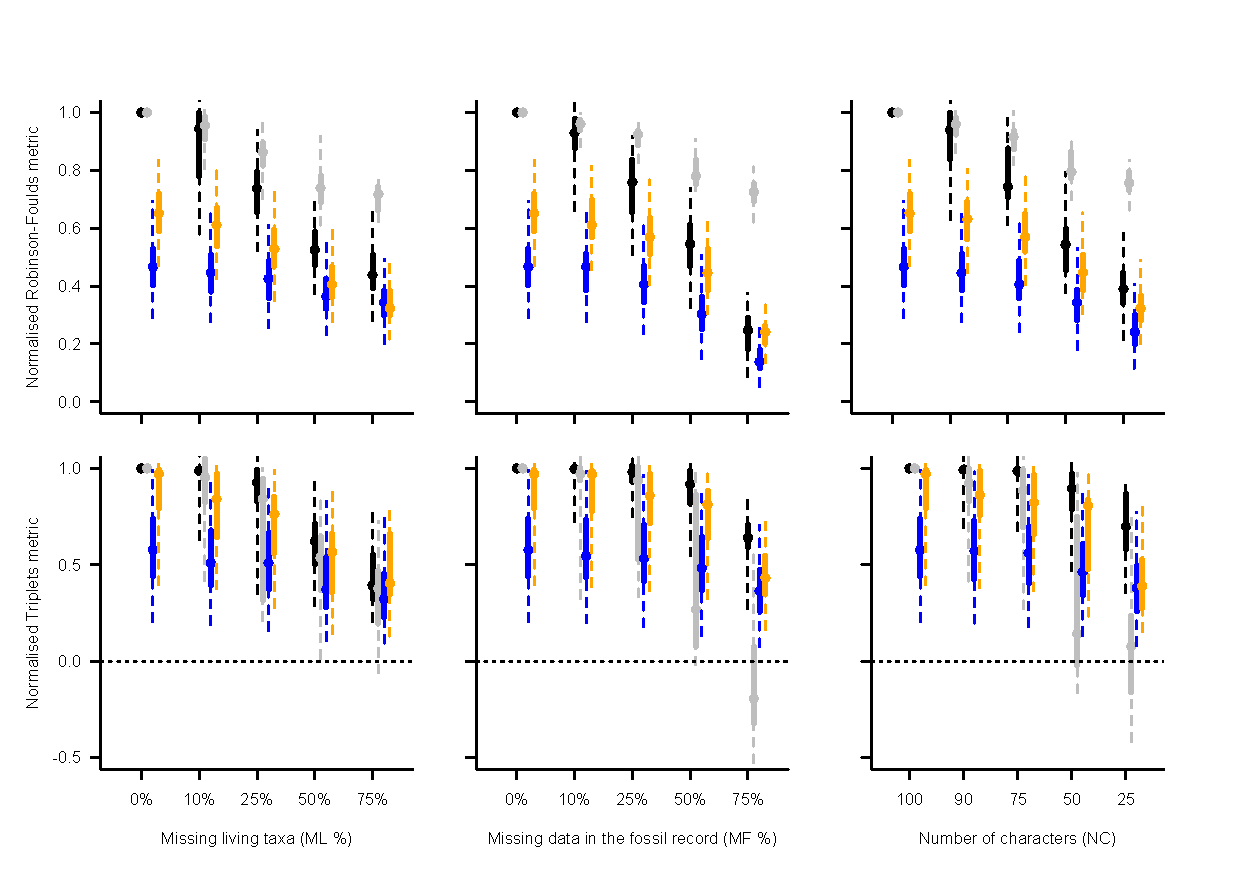
\includegraphics[width=1\textwidth]{TEM/Figures/Fig4_revised.pdf}
\caption[Effects of increasing missing data on topological recovery]{\textbf{The effects of increasing missing data on topological recovery} using Maximum Likelihood trees (black), Bayesian consensus trees (grey), Maximum Likelihood bootstrap trees (blue) and Bayesian posterior tree distributions (orange). The percentage of missing data for each parameter ($M_{L}$, $M_{F}$ and $N_{C}$) is shown on the x axis. Topological recovery was measured using two different tree comparison metrics: Normalised Robinson-Foulds metric (upper row) and Normalised Triplets metric (lower row). The graph shows the modal value (points), and the 50\% (thick solid lines) and 95\% (thin dashed lines) confidence intervals of the distributions of the tree comparison metric for each missing data parameter and tree inference method.}
\label{Fig_Results-permeth_perparam} 
\end{figure}

\begin{figure}[!ht]
\centering
    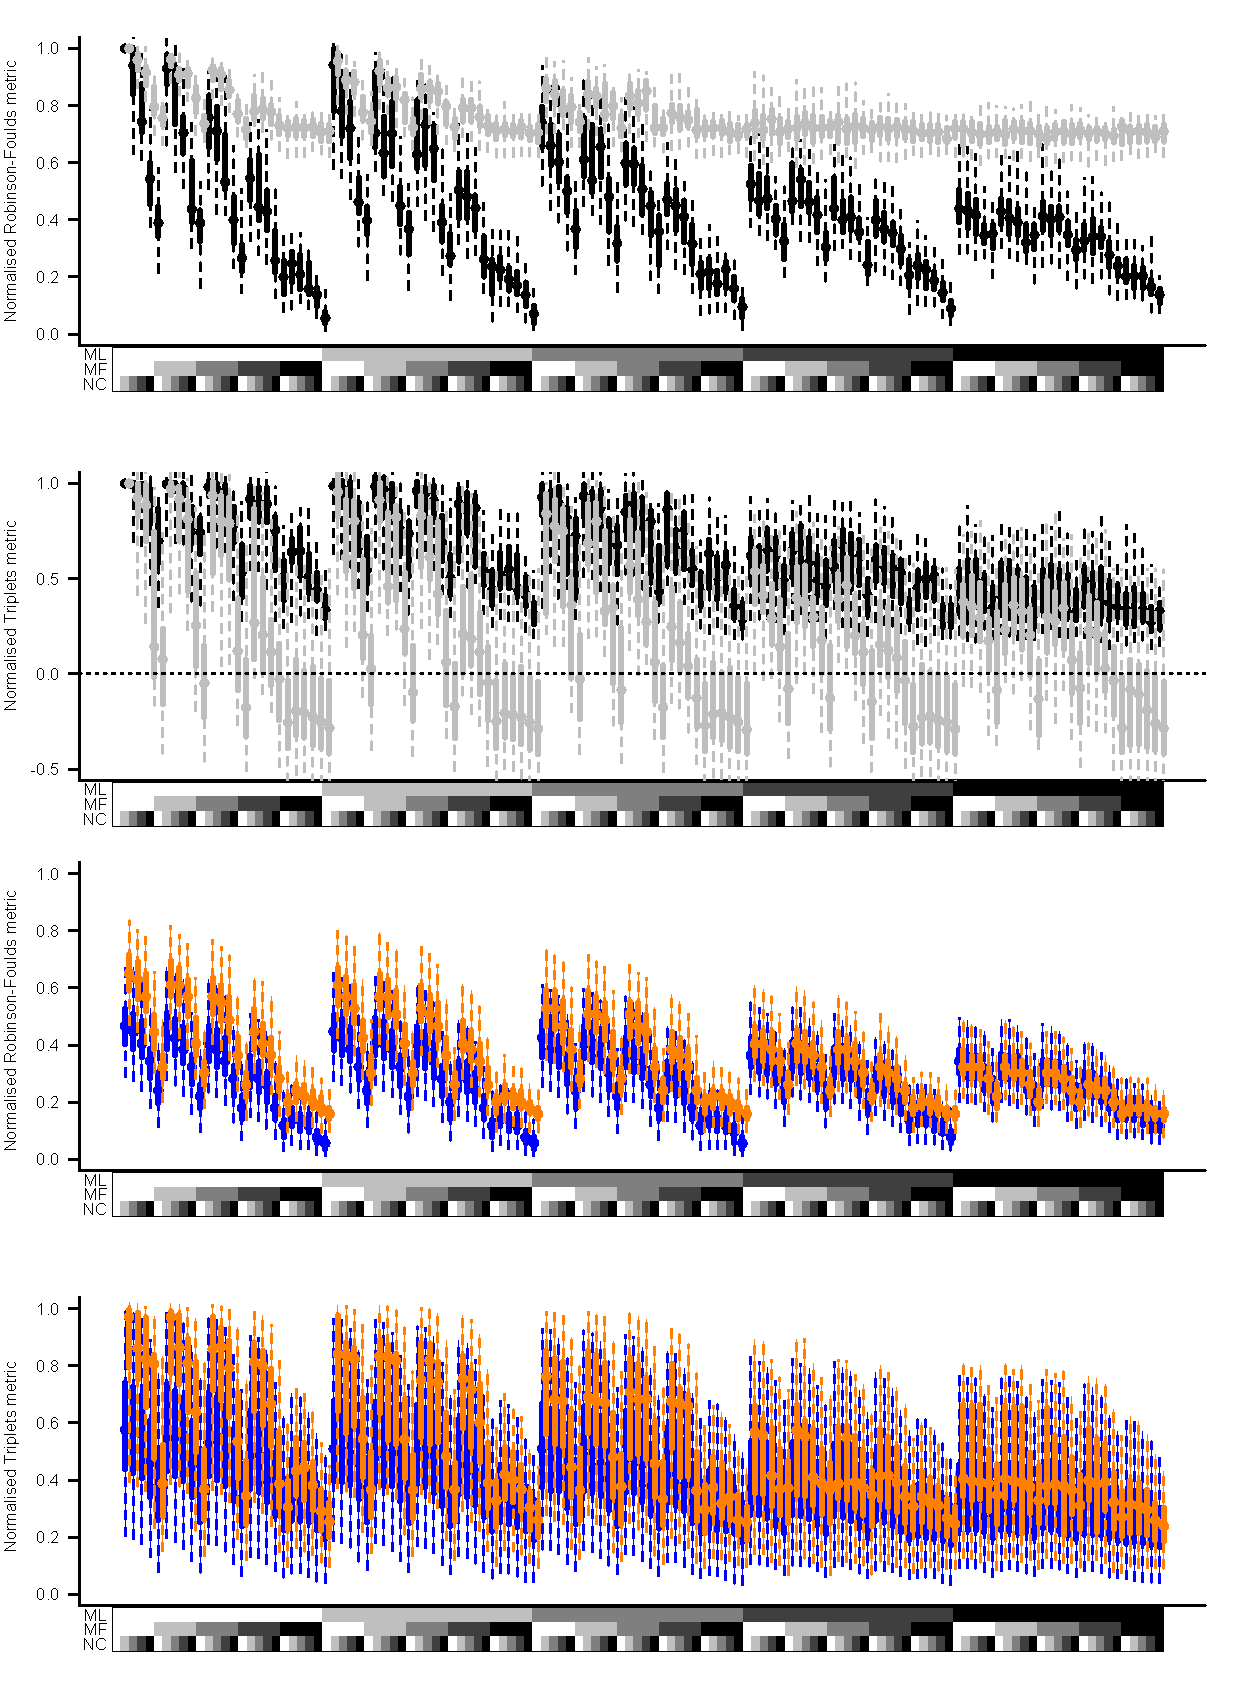
\includegraphics[width=0.9\textwidth]{TEM/Figures/Fig5_with_appendix.pdf}
\caption[Effects of increasing missing data on topological recovery with parameters combination]{\textbf{The effects of increasing missing data on topological recovery} using Maximum Likelihood trees (black), Bayesian consensus trees (grey), Maximum Likelihood Bootstrap trees (orange) and Bayesian posterior tree distribution (blue). The x axis shows the percentage of missing data from 0\% (white) to 75\% (black) for the two parameters: $M_{L}$ (upper line), $M_{F}$ (middle line) and number of characters from 100 to 25 for the parameter $N_{C}$ (lower line). Topological recovery was measured using two different tree comparison metrics: Normalised Robinson-Foulds metric (upper row) and Normalised Triplets metric (lower row). The graph shows the modal value (points), and the 50\% (thick solid lines) and 95\% (thin dashed lines) confidence intervals of the distributions of the tree comparison metric for each missing data parameter and tree inference method.} 
\label{Fig_Results-global_perparam}
\end{figure}

%Summary of metrics values for the ML parameter
\begin{landscape}
\begin{table}[!ht]
\caption[Summary of the tree comparisons for the $M_{L}$, $M_{F}$ and $N_{C}$ parameters.]{Summary of the comparisons between the "best" tree and the "missing-data" trees for each different tree inference method using either the Normalised Robinson-Foulds metric (RF) or the Normalised Triplets metric (Tr) for each parameters separately.}
\label{Tab_Supp_summary_metric}
\centering
\begin{tabular}{lccccccc}
  \hline
 Tree inference method & Metric & Min. & 1st Qu. & Median & Mean & 3rd Qu. & Max. \\ 
  \hline
  \multicolumn{8}{c}{\textbf{$M_{L}$ missing data parameter}}\\
  \hline
  Maximum Likelihood                    & $RF$ & 0.44 & 0.51 & 0.63 & 0.66 & 0.78 & 0.95 \\ 
                                        & $Tr$ & 0.45 & 0.56 & 0.76 & 0.74 & 0.93 & 0.99 \\ 
  Bayesian consensus                    & $RF$ & 0.71 & 0.73 & 0.80 & 0.82 & 0.88 & 0.95 \\ 
                                        & $Tr$ & 0.37 & 0.46 & 0.67 & 0.67 & 0.87 & 0.96 \\ 
  Maximum Likelihood bootstraps         & $RF$ & 0.34 & 0.37 & 0.42 & 0.41 & 0.44 & 0.46 \\ 
                                        & $Tr$ & 0.32 & 0.40 & 0.51 & 0.46 & 0.51 & 0.57 \\ 
  Bayesian posterior tree distributions & $RF$ & 0.33 & 0.41 & 0.52 & 0.50 & 0.60 & 0.65 \\ 
                                        & $Tr$ & 0.41 & 0.56 & 0.76 & 0.71 & 0.84 & 0.98 \\ 
  \hline
  \multicolumn{8}{c}{\textbf{$M_{F}$ missing data parameter}}\\
  \hline
  Maximum Likelihood                    & $RF$ & 0.23 & 0.46 & 0.64 & 0.61 & 0.79 & 0.93 \\ 
                                        & $Tr$ & 0.65 & 0.84 & 0.95 & 0.89 & 0.99 & 1.00 \\ 
  Bayesian consensus                    & $RF$ & 0.72 & 0.77 & 0.86 & 0.85 & 0.94 & 0.96 \\ 
                                        & $Tr$ & -0.16 & 0.19 & 0.63 & 0.52 & 0.96 & 0.98 \\ 
  Maximum Likelihood bootstraps         & $RF$ & 0.14 & 0.30 & 0.40 & 0.35 & 0.45 & 0.46 \\ 
                                        & $Tr$ & 0.37 & 0.49 & 0.54 & 0.51 & 0.56 & 0.57 \\ 
  Bayesian posterior tree distributions & $RF$ & 0.24 & 0.45 & 0.57 & 0.51 & 0.63 & 0.65 \\ 
                                        & $Tr$ & 0.44 & 0.81 & 0.86 & 0.82 & 0.98 & 0.98 \\ 
    \hline
  \multicolumn{8}{c}{\textbf{$N_{C}$ missing data parameter}}\\
  \hline
  Maximum Likelihood                    & $RF$ & 0.40 & 0.50 & 0.64 & 0.65 & 0.79 & 0.94 \\ 
                                        & $Tr$ & 0.70 & 0.84 & 0.93 & 0.89 & 0.99 & 1.00 \\ 
  Bayesian consensus                    & $RF$ & 0.76 & 0.79 & 0.86 & 0.86 & 0.92 & 0.96 \\ 
                                        & $Tr$ & 0.05 & 0.16 & 0.53 & 0.50 & 0.87 & 0.92 \\ 
  Maximum Likelihood bootstraps         & $RF$ & 0.25 & 0.34 & 0.42 & 0.38 & 0.45 & 0.46 \\ 
                                        & $Tr$ & 0.38 & 0.47 & 0.55 & 0.51 & 0.57 & 0.58 \\ 
  Bayesian posterior tree distributions & $RF$ & 0.32 & 0.44 & 0.58 & 0.52 & 0.62 & 0.65 \\ 
                                        & $Tr$ & 0.39 & 0.78 & 0.82 & 0.79 & 0.98 & 0.98 \\ 
  \hline
\end{tabular}
\end{table}
\end{landscape}

%Summary of the BC between pairs of methods for the ML parameter
\begin{landscape}
\begin{table}[!htb]
\caption[Bhattacharyya Coefficients of the pairwise method comparisons ($M_{L}$ and $M_{F}$).]{Bhattacharyya Coefficients of the pairwise method comparisons.
Each line summarizes the probabilities of overlap between the distributions of the ``best'' tree versus trees from each inference method (Maximum Likelihood; Bayesian consensus; Maximum Likelihood Bootstraps and Bayesian posterior trees) pooled across all combinations of missing data parameter values, using the Normalised Robinson-Foulds (RF) and Triplets (Tr) metrics. 
Values highlighted in bold are the extreme values of high or low probability of overlap between two methods. If two methods have a high probability of overlap, they have a similar ability to recover the ``correct'' tree topology.
Values $>$ 0.95 denote significantly similar distributions and values $<$ 0.05 denote significantly different distributions.}
\label{Tab_Supp_summary_BC_ML_MF}
\centering
\begin{tabular}{lccccccc}
  \hline
 Comparison &  Metric & Min. & 1st Qu. & Median & Mean & 3rd Qu. & Max. \\ 
  \hline
  \multicolumn{8}{c}{\textbf{$M_{L}$ missing data parameter}}\\
  \hline
    Maximum Likelihood \textit{vs.} Bayesian consensus                 & $RF$ & 0.30 & 0.31 & 0.69 & 0.61 & 0.77 & \textbf{1.00} \\ 
                                                                       & $Tr$ & 0.79 & 0.81 & 0.84 & 0.86 & 0.85 & \textbf{1.00} \\ 
    Maximum Likelihood \textit{vs.} Maximum Likelihood bootstraps      & $RF$ & \textbf{0.03} & 0.22 & 0.29 & 0.36 & 0.54 & 0.69 \\ 
                                                                       & $Tr$ & 0.08 & 0.42 & 0.53 & 0.51 & 0.74 & 0.78 \\ 
    Maximum Likelihood \textit{vs.} Bayesian posterior trees           & $RF$ & \textbf{0.02} & 0.49 & 0.61 & 0.51 & 0.67 & 0.74 \\ 
                                                                       & $Tr$ & 0.21 & 0.61 & 0.70 & 0.63 & 0.81 & 0.81 \\ 
    Bayesian consensus \textit{vs.} Maximum Likelihood bootstraps      & $RF$ & \textbf{0.01} & \textbf{0.02} & \textbf{0.02} & \textbf{0.02} & \textbf{0.03} & \textbf{0.04} \\ 
                                                                       & $Tr$ & 0.08 & 0.69 & 0.78 & 0.64 & 0.79 & 0.84 \\ 
    Bayesian consensus \textit{vs.} Bayesian posterior trees           & $RF$ & \textbf{0.01} & \textbf{0.02} & \textbf{0.02} & \textbf{0.04} & 0.08 & 0.09 \\ 
                                                                       & $Tr$ & 0.21 & 0.74 & 0.75 & 0.68 & 0.84 & 0.87 \\ 
    Bayesian posterior tree \textit{vs.} Maximum Likelihood bootstraps & $RF$ & 0.69 & 0.75 & 0.85 & 0.85 & \textbf{0.95} & \textbf{1.00} \\ 
                                                                       & $Tr$ & 0.91 & 0.92 & \textbf{0.96} & \textbf{0.95} & \textbf{0.97} & \textbf{0.98} \\ 
  \hline
  \multicolumn{8}{c}{\textbf{$M_{F}$ missing data parameter}}\\
  \hline
    Maximum Likelihood \textit{vs.} Bayesian consensus                 & $RF$ & \textbf{0.00} & 0.25 & 0.48 & 0.50 & 0.76 & \textbf{1.00} \\ 
                                                                       & $Tr$ & 0.38 & 0.69 & 0.75 & 0.72 & 0.80 & \textbf{1.00} \\ 
    Maximum Likelihood \textit{vs.} Maximum Likelihood bootstraps      & $RF$ & \textbf{0.03} & 0.18 & 0.32 & 0.36 & 0.47 & 0.77 \\ 
                                                                       & $Tr$ & 0.08 & 0.34 & 0.40 & 0.38 & 0.53 & 0.55 \\ 
    Maximum Likelihood \textit{vs.} Bayesian posterior trees           & $RF$ & \textbf{0.02} & 0.47 & 0.71 & 0.60 & 0.86 & 0.94 \\ 
                                                                       & $Tr$ & 0.21 & 0.54 & 0.62 & 0.56 & 0.64 & 0.80 \\ 
    Bayesian consensus \textit{vs.} Maximum Likelihood bootstraps      & $RF$ & \textbf{0.00} & \textbf{0.00} & \textbf{0.01} & \textbf{0.01} & \textbf{0.01} & \textbf{0.03} \\ 
                                                                       & $Tr$ & 0.08 & 0.38 & 0.54 & 0.49 & 0.70 & 0.75 \\ 
    Bayesian consensus \textit{vs.} Bayesian posterior trees           & $RF$ & \textbf{0.00} & \textbf{0.02} & \textbf{0.02} & \textbf{0.02} & \textbf{0.04} & \textbf{0.04} \\ 
                                                                       & $Tr$ & 0.21 & 0.29 & 0.66 & 0.54 & 0.72 & 0.82 \\ 
    Bayesian posterior tree \textit{vs.} Maximum Likelihood bootstraps & $RF$ & 0.69 & 0.69 & 0.72 & 0.71 & 0.72 & 0.72 \\ 
                                                                       & $Tr$ & 0.91 & 0.91 & 0.91 & 0.93 & 0.92 & \textbf{0.98} \\ 
   \hline  
\end{tabular}
\end{table}
\end{landscape}

%Summary of the BC between pairs of methods for the MC parameter
\begin{landscape}
\begin{table}[!htb]
\caption[Bhattacharyya Coefficients of the pairwise method comparisons ($N_{C}$ and all parameters combination).]{Bhattacharyya Coefficients of the pairwise method comparisons.
Each line summarizes the probabilities of overlap between the distributions of the ``best'' tree versus trees from each inference method (Maximum Likelihood; Bayesian consensus; Maximum Likelihood Bootstraps and Bayesian posterior trees) pooled across all combinations of missing data parameter values, using the Normalised Robinson-Foulds (RF) and Triplets (Tr) metrics. 
Values highlighted in bold are the extreme values of high or low probability of overlap between two methods. If two methods have a high probability of overlap, they have a similar ability to recover the ``correct'' tree topology.
Values $>$ 0.95 denote significantly similar distributions and values $<$ 0.05 denote significantly different distributions.}
\label{Tab_Supp_summary_BC_NC_Global}
\centering
\begin{tabular}{lccccccc}
  \hline
 Comparison &  Metric & Min. & 1st Qu. & Median & Mean & 3rd Qu. & Max. \\  
  \hline
  \multicolumn{8}{c}{\textbf{$N_{C}$ missing data parameter}}\\
  \hline
    Maximum Likelihood \textit{vs.} Bayesian consensus                 & $RF$ & \textbf{0.03} & 0.32 & 0.66 & 0.55 & 0.75 & \textbf{1.00} \\ 
                                                                       & $Tr$ & 0.51 & 0.69 & 0.80 & 0.76 & 0.80 & \textbf{1.00} \\ 
    Maximum Likelihood \textit{vs.} Maximum Likelihood bootstraps      & $RF$ & \textbf{0.03} & 0.17 & 0.21 & 0.31 & 0.46 & 0.68 \\ 
                                                                       & $Tr$ & 0.08 & 0.31 & 0.39 & 0.39 & 0.56 & 0.61 \\ 
    Maximum Likelihood \textit{vs.} Bayesian posterior trees           & $RF$ & \textbf{0.02} & 0.44 & 0.47 & 0.52 & 0.78 & 0.90 \\ 
                                                                       & $Tr$ & 0.21 & 0.52 & 0.59 & 0.55 & 0.66 & 0.77 \\ 
    Bayesian consensus \textit{vs.} Maximum Likelihood bootstraps      & $RF$ & \textbf{0.00} & \textbf{0.01} & \textbf{0.01} & \textbf{0.02} & \textbf{0.02} & \textbf{0.03} \\ 
                                                                       & $Tr$ & 0.08 & 0.47 & 0.62 & 0.51 & 0.66 & 0.73 \\ 
    Bayesian consensus \textit{vs.} Bayesian posterior trees           & $RF$ & \textbf{0.00} & \textbf{0.02} & \textbf{0.04} & \textbf{0.04} & 0.05 & 0.06 \\ 
                                                                       & $Tr$ & 0.21 & 0.45 & 0.64 & 0.57 & 0.74 & 0.79 \\ 
    Bayesian posterior tree \textit{vs.} Maximum Likelihood bootstraps & $RF$ & 0.69 & 0.73 & 0.73 & 0.76 & 0.81 & 0.86 \\ 
                                                                       & $Tr$ & 0.91 & 0.92 & 0.93 & 0.94 & \textbf{0.96} & \textbf{0.99} \\
  \hline
  \multicolumn{8}{c}{\textbf{All missing data parameters combined}}\\
  \hline
    Maximum Likelihood \textit{vs.} Bayesian consensus                 & $RF$ & \textbf{0.00} & \textbf{0.00} & 0.10 & 0.20 & 0.32 & \textbf{1.00} \\ 
                                                                       & $Tr$ & 0.34 & 0.49 & 0.61 & 0.62 & 0.75 & \textbf{1.00} \\ 
    Maximum Likelihood \textit{vs.} Maximum Likelihood bootstraps      & $RF$ & \textbf{0.03} & 0.54 & 0.69 & 0.64 & 0.77 & \textbf{0.98} \\ 
                                                                       & $Tr$ & 0.08 & 0.57 & 0.65 & 0.64 & 0.73 & 0.82 \\ 
    Maximum Likelihood \textit{vs.} Bayesian posterior trees           & $RF$ & \textbf{0.02} & 0.74 & 0.80 & 0.79 & 0.89 & \textbf{0.98} \\ 
                                                                       & $Tr$ & 0.21 & 0.67 & 0.73 & 0.72 & 0.77 & 0.84 \\ 
    Bayesian consensus \textit{vs.} Maximum Likelihood bootstraps      & $RF$ & \textbf{0.00} & \textbf{0.00} & \textbf{0.00} & \textbf{0.01} & \textbf{0.01} & \textbf{0.04} \\ 
                                                                       & $Tr$ & 0.08 & 0.38 & 0.59 & 0.57 & 0.73 & 0.84 \\ 
    Bayesian consensus \textit{vs.} Bayesian posterior trees           & $RF$ & \textbf{0.00} & \textbf{0.00} & \textbf{0.01} & \textbf{0.02} & \textbf{0.04} & 0.11 \\ 
                                                                       & $Tr$ & 0.21 & 0.36 & 0.56 & 0.55 & 0.74 & 0.87 \\ 
    Bayesian posterior tree \textit{vs.} Maximum Likelihood bootstraps & $RF$ & 0.50 & 0.77 & 0.85 & 0.85 & \textbf{0.96} & \textbf{1.00} \\ 
                                                                       & $Tr$ & 0.91 & \textbf{0.96} & \textbf{0.98} & \textbf{0.97} & \textbf{0.99} & \textbf{1.00} \\   
   \hline
\end{tabular}
\end{table}
\end{landscape}

\subsection{Combined effect of missing data parameters}
As expected, our ability to recover the ``best'' tree topology is worst when each parameter contains the maximum amount of missing data (i.e. $M_{L}$ = 75\%, $M_{F}$ = 75\% and $N_{C}$ = 75\%), and best when there is no missing data (i.e. $M_{L}$ = 0\%, $M_{F}$ = 0\%, $N_{C}$ = 0\%; Fig. \ref{Fig_Results-global_perparam}; Table \ref{Tab_Supp_summary_metric}).
Fig. \ref{Fig_Results-paircomp_within1} and \ref{Fig_Results-paircomp_within2} shows the similarity of distributions of tree metrics in a triangular matrix with the values of each pairwise Bhattacharyya Coefficient coloured according to their values (orange when the distributions overlap completely, Bhattacharyya Coefficient = 1, and blue when they do not, Bhattacharyya Coefficient = 0). 

Using both Normalised Robinson-Foulds and Normalised Triplets metrics from the Bayesian consensus trees, the parameter combination with no missing data (i.e. $M_{L}$ = 0\%, $M_{F}$ = 0\%, $N_{C}$ = 100) is always the most dissimilar to all the other parameter combinations (thin deep blue line at the base of Fig. \ref{Fig_Results-paircomp_within1}C-D).
The Normalised Robinson-Foulds metric (median Bhattacharrya coefficient = 0.79; blue regions in Fig. \ref{Fig_Results-paircomp_within1}C), however, displays more dissimilarities than the Normalised Triplets metric (median Bhattacharrya coefficient = 0.81; blue regions in Fig. \ref{Fig_Results-paircomp_within1}D).
The orange upper triangle in Fig. \ref{Fig_Results-paircomp_within1}A shows a high probability of overlap of the Normalised Robinson-Foulds metric for the trees with the $M_{L}$ parameter $\geq$ 50\% (Fig. \ref{Fig_Results-paircomp_within1}A).
Once $M_{L}$ $\geq$ 50\%, there is no additional effect of $M_{F}$ and $N_{C}$, regardless of the amount of missing data in these parameters (Fig. \ref{Fig_Results-paircomp_within1}A).
Likewise, once $N_{C}$ $<$ 50, there is no additional effect of $M_{L}$ and $M_{F}$ as denoted by the high probability of Normalised Robinson-Foulds metric overlap (horizontal orange stripes between the blue regions Fig. \ref{Fig_Results-paircomp_within1}A).
In Fig. \ref{Fig_Results-global_perparam} for the Normalised Robinson-Foulds metric, this can be interpreted as the overlap between the distributions once $M_L$=50\%.

For all combinations of missing data parameters and tree comparison metrics, the Maximum Likelihood bootstrap trees and the Bayesian posterior tree distributions perform very similarly (median Bhattacharrya Coefficient = 0.85 and 0.98, using Normalised Robinson-Foulds metric or Normalised Triplets metric respectively; Tables \ref{Tab_Supp_summary_BC_ML_MF} and \ref{Tab_Supp_summary_BC_NC_Global}).
These two methods, however, perform worse than the Bayesian consensus trees using Normalised Robinson-Foulds metric (median Bhattacharrya Coefficient = 0 and 0.01, for the Maximum Likelihood bootstrap trees and the Bayesian posterior tree distribution respectively; \ref{Tab_Supp_summary_BC_ML_MF} and \ref{Tab_Supp_summary_BC_NC_Global}; Fig. \ref{Fig_Results-permeth_perparam}).

\begin{figure}[!]
\centering
    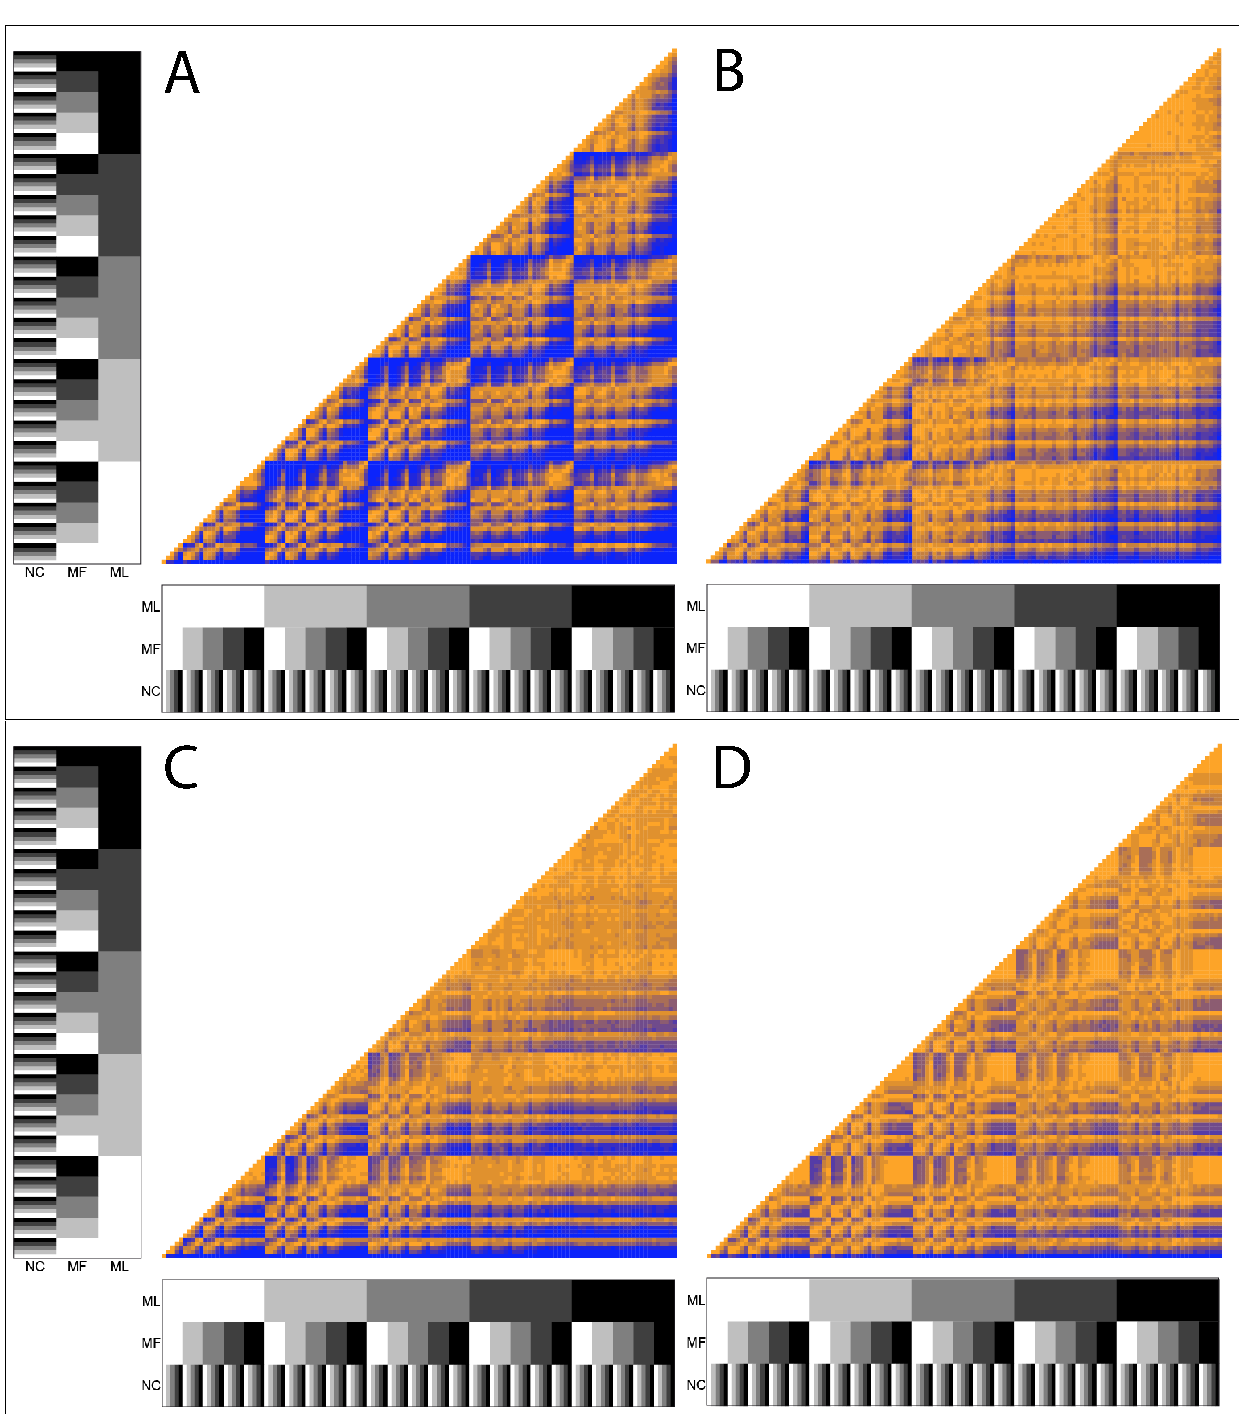
\includegraphics[width=0.95\textwidth]{TEM/Figures/Fig6_double.pdf}
\caption[Effects of missing data on topological recovery using Maximum Likelihood and Bayesian consensus trees]{\textbf{The effects of missing data on topological recovery using Maximum Likelihood and Bayesian consensus trees.} Both axes show the percentage of missing data from 0\% (white) to 75\% (black) for the three parameters: $M_{L}$ (upper line), $M_{F}$ (middle line) and $N_{C}$ (lower line). The first row (A and B) corresponds to the Maximum Likelihood trees and the second row (C and D) to the Bayesian consensus trees. The topological recovery is measured as (A and C) the Normalised Robinson-Foulds metric and (B and D) the Normalised Triplets metric calculated using the Bhattacharyya Coefficient. The Bhattacharyya Coefficient values are indicated using a color gradient ranging from low probability of overlap in blue, to high probability of overlap in orange. Blue regions denote a poor overlap in Normalised metric values between the different parameter combinations (i.e. the parameters have a strong effect on the metric and thus the topological recovery). Conversely, orange regions denote a high overlap in Normalised metric values between the different parameter combinations (i.e. the parameters have a weak effect on the metric and thus the topological recovery).}
\label{Fig_Results-paircomp_within1}
\end{figure}

\begin{figure}[!]
\centering
    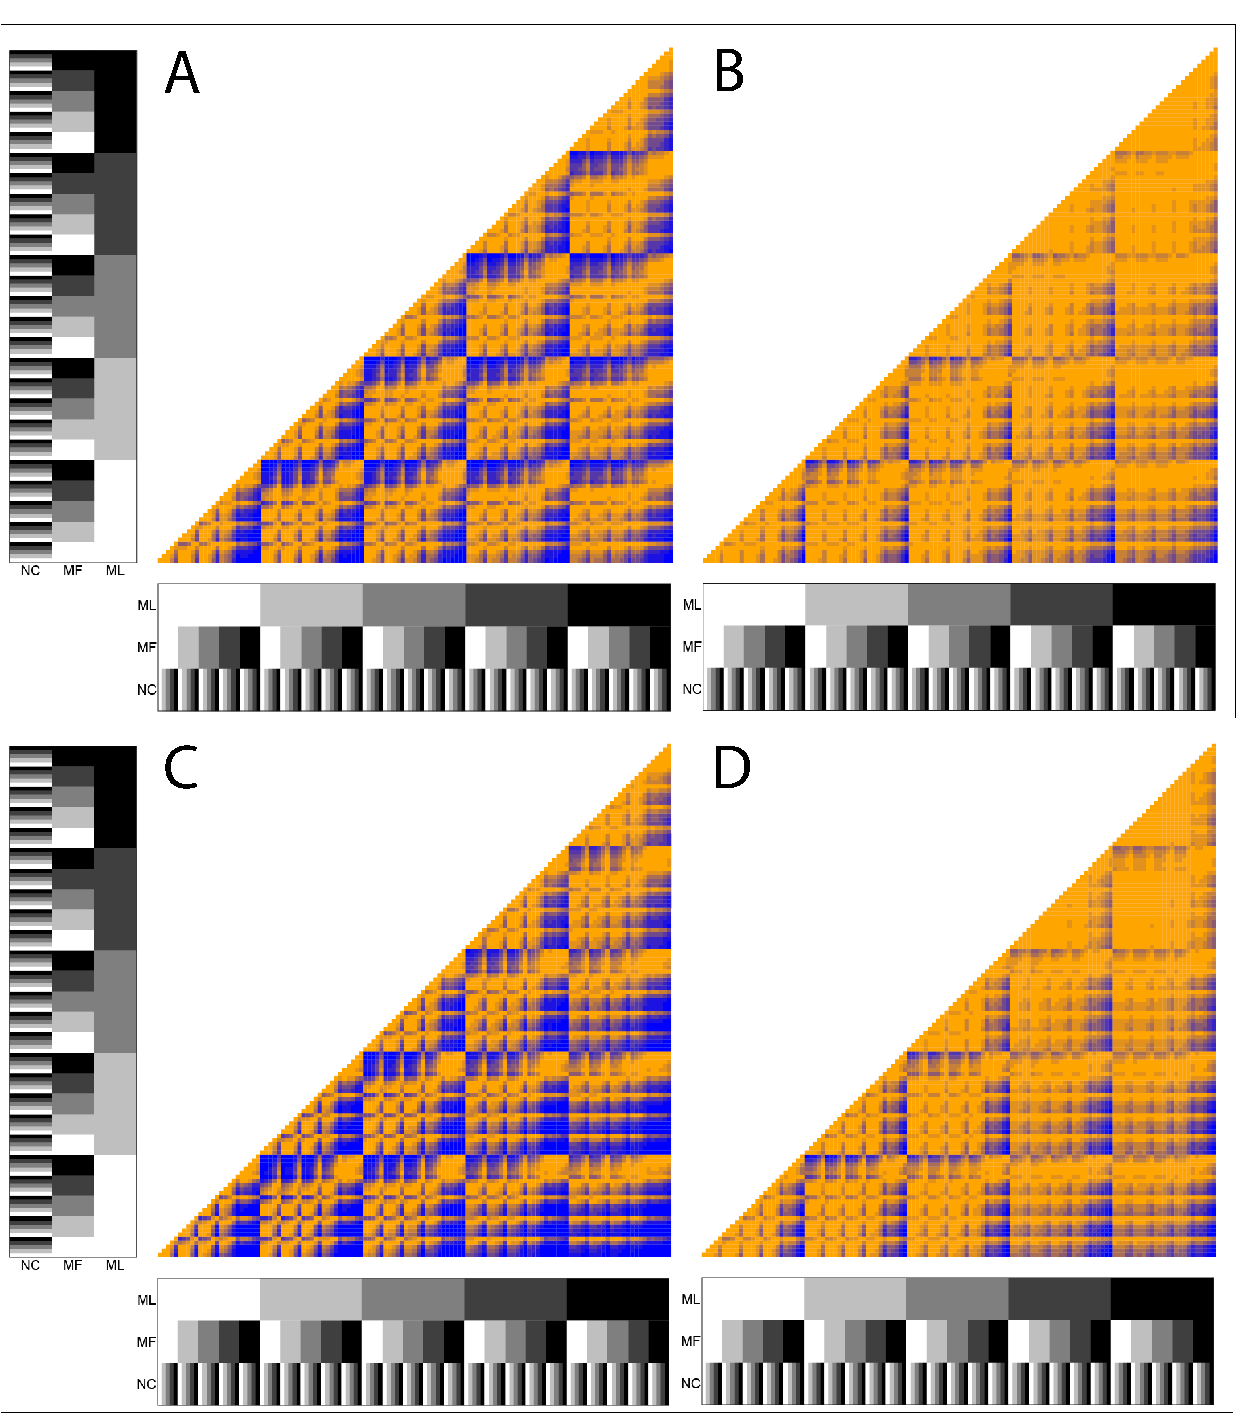
\includegraphics[width=0.95\textwidth]{TEM/Figures/Fig7_double.pdf}
\caption[Effects of missing data on topological recovery using Maximum Likelihood bootstrap and Bayesian posterior distribution trees]{\textbf{The effects of missing data on topological recovery using Maximum Likelihood bootstrap and Bayesian posterior distribution trees.} Both axes show the percentage of missing data from 0\% (white) to 75\% (black) for the three parameters: $M_{L}$ (upper line), $M_{F}$ (middle line) and $N_{C}$ (lower line). The first row (A and B) corresponds to the Maximum Likelihood bootstrap trees and the second row (C and D) to the Bayesian posterior distribution trees. The topological recovery is measured as (A and C) the Normalised Robinson-Foulds metric and (B and D) the Normalised Triplets metric calculated using the Bhattacharyya Coefficient. The Bhattacharyya Coefficient values are indicated using a color gradient ranging from low probability of overlap in blue, to high probability of overlap in orange. Blue regions denote a poor overlap in Normalised metric values between the different parameter combinations (i.e. the parameters have a strong effect on the metric and thus the topological recovery). Conversely, orange regions denote a high overlap in Normalised metric values between the different parameter combinations (i.e. the parameters have a weak effect on the metric and thus the topological recovery).}
\label{Fig_Results-paircomp_within2}
\end{figure}



%---------------------------------------------
%
%       Discussion
%
%---------------------------------------------


\section{Discussion}

Our results show that the ability to recover the ``best'' tree topology in a Total Evidence framework decreases as the amount of missing data increases, regardless of how data were removed or the method of tree inference used.
These factors, however, affected topological recovery in different ways and to different extents.
Decreasing the number of living taxa with morphological data ($M_{L}$) and the overall number of morphological characters in the matrix ($N_{C}$) had worst effects on topological recovery (Fig. \ref{Fig_Results-paircomp_within1} and \ref{Fig_Results-paircomp_within2}).
Additionally, using Bayesian consensus trees recovered the ``best'' tree topology more consistently than using Maximum Likelihood trees or Bayesian posterior tree distributions (Fig. \ref{Fig_Results-global_perparam}, Fig. \ref{Fig_Results-paircomp_within1}, Table \ref{Tab_Supp_summary_BC_ML_MF} and \ref{Tab_Supp_summary_BC_NC_Global}).
As seen in previous studies, our results show that the amount of missing data are not a problem \textit{per se} for Total Evidence methods, as long as enough living and fossil taxa in the matrix have data for overlapping morphological characters \citep[e.g.][]{kearneyfragmentary2002,wiensmissing2003,rouresite-specific2011,pattinsonphylogeny2014}.

\subsection{Individual effects of missing data parameters}
\subsubsection*{Missing data for living taxa ($M_{L}$)}
When the number of living taxa with morphological data ($M_{L}$) decreases, entire rows of data are being removed from the living taxa part of the matrix.
Because living taxa still have molecular characters available for phylogenetic inference (see Methods), even if they have no morphological data, the relationships among them will always be fairly well-resolved (depending on the phylogenetic signal from the molecular part of the matrix).
This missing data parameter, however, has a huge influence on the placement of fossil taxa because a decrease in the $M_{L}$ parameter reduces the amount of overlapping data among the living and fossil taxa, meaning there is no part of the living taxa tree that the fossils can branch off.

\subsubsection*{Missing data for fossil taxa ($M_{F}$)}
When the overall proportion of data for the fossil taxa ($M_{F}$) decreases, this also reduces the probability of morphological characters for fossil taxa overlapping with the ones for living taxa.
This can lead to difficulties for the placement of certain taxa in the tree.
It is important, however, to note that even though the number of displaced wildcard taxa increases (i.e. decrease of Normalised Triplets metric) with increasing missing data in this parameter, clade conservation (i.e. Normalised Robinson-Foulds metric) is still relatively good (mode = 0.72) when the proportion of missing data are high ($M_{F}$ = 75\%).
These results are in agreement with \cite{manosphylogeny2007} where as few as 16 characters were sufficient for correctly assigning artificial fossils to their correct clade.

The effect of the missing data in the fossil record ($M_{F}$) is less than the effect of the $M_{L}$ parameter on clade conservation (Normalised Robinson-Foulds metric) but greater on the displacement of wildcard taxa (Normalised Triplets metric; Fig. \ref{Fig_Results-permeth_perparam} and Fig. \ref{Fig_Results-global_perparam}).
This is related to the fact that the Bayesian consensus tree is built using a majority consensus rule.
When the fossil taxa have less data (e.g. $M_{F}$ = 75\%) they will tend to branch with any taxon in the clade that shares most characters with the fossils.
Therefore a majority consensus position is unlikely to exist (i.e. every branching position is represented in $<$ 50\% of the trees in the Bayesian posterior distribution) and the fossil taxa will form a polytomy at the base of the clade.
In this case, the Normalised Robinson-Foulds metric will decrease when the fossil is present near the tips but affects the clade conservation less when fossils are near the root.
Conversely, because a fossil in a high taxonomic level clade has many chances to branch on different nodes within the clade, it will be more likely to act as a wildcard taxon and decrease the Normalised Triplets metric.
Therefore, the $M_{F}$ parameter is likely to affect the Normalised Robinson-Foulds metric less than the Normalised Triplets metric for the Bayesian consensus trees.
Conversely, the same scenario in a Maximum Likelihood framework will lead to a dichotomous branching of the fossils but with low bootstrap support ($<$ 50).
In other words, the Bayesian consensus tree allows a fossil taxon with few data to be placed with a higher confidence at a lower taxonomic level than the Maximum Likelihood tree, where the fossil will be placed with lower confidence at a higher taxonomic level.
We argue that using the Bayesian consensus tree topology is preferable because it is more conservative \citep[e.g.][]{pattinsonphylogeny2014}.

\subsubsection*{Number of morphological characters ($N_{C}$)}
Reducing the overall number of morphological characters reduces the probability of their overlap among the taxa in the matrix, and therefore decreases our ability to recover the ``best'' tree topology.
We expected the decrease in this parameter to have an effect twice as large as that for the $M_{L}$ and $M_{F}$ parameters, because removing 10\% of the data for the fossil or living taxa only removes 5\% of data from the whole matrix (because this parameter affects only half of the taxa present in the matrix).
Conversely, removing 10\% of morphological characters (i.e. $N_{C}$ = 90) genuinely removes 10\% of data in the matrix.
Nonetheless, the effect of removing characters on the ability to recover the ``best'' tree topology is of the same order of magnitude as for the other two parameters (Fig. \ref{Fig_Results-permeth_perparam}).
We suspect this again reflects the importance of overlapping characters, as opposed to the number of characters \textit{per se}.

Additionally, the number of morphological characters determines the size of the matrix.
This can affect our ability to recover the ``best'' tree topology through: (1) the incongruence of phylogenetic signal among morphological and molecular data; and/or (2) homoplasy.
The incongruence of phylogenetic signal between morphological and molecular data has previously been demonstrated to be more important in small morphological matrices (\citealt{bremer1992phylogeny,patterson1993congruence}; see \citealt{masters2002lack} for an empirical example).
The sizes of our data matrices were constrained by the performance of our protocol: to reduce the computational time of our analysis to a reasonable level (150 CPU years), we ran our simulations on modestly-sized matrices of 1000 molecular characters and 100 morphological characters.
Therefore, part of the decrease of the Normalised Robinson-Foulds metric and the Normalised Triplets metric in our simulations could be due to conflicting phylogenetic signal among morphological and molecular data in our matrices (Fig. \ref{Fig_Results-permeth_perparam} and Fig. \ref{Fig_Results-permeth_perparam}).
Although these matrices are an order of magnitude smaller than some published matrices \citep[e.g.][]{springermacroevolutionary2012,ni2013oldest}, they are still within the size range of more modestly-sized empirical matrices \citep[e.g.][]{kellymolecular2014, sallam2011craniodental}.
Therefore, our simulations reflect realistic parameters.
Nonetheless, the use of probabilistic methods (i.e. Maximum Likelihood or Bayesian) and the M\textit{kv} model \citep{lewisa2001} has been previously demonstrated to partially resolve this issue \citep{wrightbayesian2014}.

\subsection{Combined effect of missing data parameters}
As expected, when combining the missing data parameters, our ability to recover the ``best'' tree topology is affected in the same way as for the parameters individually: the Normalised Robinson-Foulds metric and the Normalised Triplets metric are higher when all the missing data parameters have few missing data (i.e. $M_{L}$ = 0\%, $M_{F}$ = 0\%, $N_{C}$ = 100) and lower when they have a larger proportion of missing data (i.e. $M_{L}$ = 75\%, $M_{F}$ = 75\% and $N_{C}$ = 25; Fig. \ref{Fig_Results-global_perparam}).
It is important, however, to notice that the effect of each parameter is not additive.
Surprisingly, the number of missing living taxa with morphological data ($M_{L}$) and the overall number of missing morphological characters ($N_{C}$), have a bigger effect than the amount of missing data for the fossil taxa ($M_{F}$).
For any additional missing living taxa with morphological data ($M_L$) beyond 50\%, there is no difference among trees with any combination of the other parameters ($M_F$ and $N_C$; Fig. \ref{Fig_Results-paircomp_within1}).
In other words, when the number of missing living taxa reaches 50\%, neither the amount of missing data in the fossil record ($M_F$), nor the number of characters in the matrix ($N_C$) affect topology.
A similar effect can be observed when the $N_C$ parameter reaches 50 characters (Fig. \ref{Fig_Results-paircomp_within1}).
This has important practical implications, especially for the best strategy to improve topology by collecting more morphological data (see below).

\subsection{Effects of tree inference methods}
Variation in our ability to recover the ``best'' tree topology depends heavily on the tree inference method (Fig. \ref{Fig_Results-permeth_perparam} and Fig. \ref{Fig_Results-global_perparam}).
For morphological data, previous studies have shown some superiority of probabilistic tree inference methods with simple evolutionary models such as the M\textit{kv} model \citep{lewisa2001} over parsimony methods (\citealp{wrightbayesian2014}; but see \citealp{spencerefficacy2013}).
This is, however, the first study, to our knowledge, to compare the performance of the M\textit{kv} model \citep{lewisa2001} for recovering the ``best'' tree topology using Maximum Likelihood and Bayesian methods in a Total Evidence framework.
Our results show that the topology of the Bayesian consensus tree is always closer to the ``best'' tree topology than the ``best'' Maximum Likelihood tree (Fig. \ref{Fig_Results-global_perparam}).
Note that the methodological choice of using the ``true'' tree as a starting tree for the Bayesian Inference rather than a random starting tree (see Methods), had no significant effect on topological recovery (see Supplementary data A.1).
As described above, this is because the Bayesian consensus tree allows a fossil taxon with few data to be placed with a higher confidence at a lower taxonomic level than the Maximum Likelihood tree.
This may also be because the ``best'' Bayesian consensus trees are not completely resolved, thus will always be more similar to the ``missing data" trees than a completely resolved tree like the ``best'' Maximum Likelihood tree.
Nonetheless, we minimized the probability of unresolved ``best'' trees in our Bayesian analyses by only using datasets with strong phylogenetic signal (see Methods).

The Bayesian consensus trees, however, perform poorly for the Normalised Triplets metric: some parameter combinations, especially when the $M_F$ parameter reaches 75\% missing data, lead to negative values (Fig. \ref{Fig_Results-global_perparam}).
A Normalised Triplets metric value below 0 means that the placement of some taxa is worse than expected by just randomly placing this taxon in the tree.
This can be interpreted as the absence of comparable triplets between some of the ``missing data" trees and ``best'' trees.
Even if clades are conserved (Fig. \ref{Fig_Results-global_perparam}), the resolution within them can be poor to non-existent when a large proportion of data are missing (i.e. 75\%).
In such cases, the fossil taxa are equally likely to be placed in any of the clades that they share the most characters with.
These results are in agreement with previous studies that have showed that missing data can cause problems for recovering ``correct'' topologies, especially for small matrices of 100 characters \citep{wiensmissing2003}.
It is important to note, however, that this effect can be reduced by increasing the number of characters \citep{wiensmissing2003}.

It is also worth noting that across all our analyses, the topologies of the Maximum Likelihood bootstrap trees and the Bayesian posterior trees distribution were always further from the ``best'' tree topology than Maximum Likelihood and Bayesian consensus trees.
This was true even when no morphological data were missing ($M_{L}$ = 0\%; $M_{F}$ = 0\%, $N_{C}$ = 100; Fig. \ref{Fig_Results-permeth_perparam}).
This reflects the fact that it is difficult to compare two distributions of trees, and each comparison between a set of ``missing data" trees and a set of the ``best'' trees involved 1000 random pairwise comparisons rather than just one.
Additionally, the Bayesian posterior trees performed more poorly than the Bayesian consensus tree (Fig. \ref{Fig_Results-permeth_perparam}, Tables \ref{Tab_Supp_summary_metric}, \ref{Tab_Supp_summary_BC_ML_MF} and \ref{Tab_Supp_summary_BC_NC_Global}).
This may be because the Bayesian posterior trees are always resolved and thus more likely to contain incorrectly resolved nodes (i.e. decreasing the Normalised Robinson-Foulds metric).
Conversely, the Bayesian consensus trees might not resolve nodes that are poorly supported and thus are more likely to contain only correctly resolved nodes (i.e. increasing the Normalised Robinson-Foulds metric).


\subsection{Practical implications}
Our missing data parameters illustrate different sources of missing data in empirical matrices as follows: ($M_{L}$) the paucity of coded morphological characters for living taxa; ($M_{F}$) the missing data for fossils (or parts of fossils) that have not been preserved in the fossil record; and ($N_{C}$) characters that have not been coded across living and fossil species, perhaps due to difficulties in coding or poor preservation of the feature in collections.
Filling these gaps in empirical Total Evidence matrices should lead to a substantial increase in our ability to recover the ``best'' tree topology.
We can increase the number of living taxa with coded morphological characters by increasing research efforts in this area, and encouraging use of our vast natural history collections.
Increasing data for fossil species is harder, since it depends on fossil preservation biases and new fossil discoveries.
Gaps in the matrix, however, can be filled with efforts in palaeontological field work that can potentially lead to future discoveries of exceptionally preserved fossils \citep[e.g.][]{ni2013oldest}.
Fortunately, although these data are the most difficult to collect, they also have the least influence on whether our simulations recover the ``best'' tree topology (Fig. \ref{Fig_Results-paircomp_within1}).
Finally, although increasing the number of coded characters is relatively straightforward, the amount of time it takes to build a morphological matrix increases directly with the number of characters involved.
One solution to this problem may be to engage with collaborative data collection projects through web portals such as \textit{MorphoBank} \citep{morphobank}, so that no single individual collects all the data.

Another practical implication of our results regards the tree inference methods.
Because the Bayesian consensus trees consistently recovered topologies closer to the ``best'' tree topology than the Maximum Likelihood trees, we advise that where a topological constraint is needed, Bayesian consensus trees should be used.
This may apply to tree inferences using the Total Evidence method such as tip-dating \citep[e.g.][]{ronquista2012,Wood01032013,BEASTmaster}.
It is, however, possible that including dating information during tree inference could also improve the accuracy of the Bayesian posterior tree distribution, so a fixed topology should be used with caution.
Using the Bayesian consensus tree rather than the Maximum Likelihood can also reduce the number of false positive topologies \citep[\textit{sensu}][]{Swofford2001}.
As shown in Fig. \ref{Fig_Results-global_perparam} and discussed in the section above (Effects of tree inference methods), the Bayesian consensus tree is more likely to not resolve poorly supported nodes due to missing data than the Maximum Likelihood tree that is more likely to incorrectly resolve such nodes (i.e. creating a false positive node).
Note, however, that we do not suggest discarding the Bayesian posterior tree distributions even though they performed poorly in recovering the ``best'' tree topology in our simulations (this can probably be traced to the difficulties comparing distributions of trees; see above).
These trees will be invaluable for phylogenetic comparative analyses.
For example a sub-sample of posterior tree distributions can be used to assess macroecological questions while better taking into account topological uncertainty (e.g. \citealt{fritzdiversity2013} and \citealt{jetzthe2012} used in \citealt{healy2014}).

\section{Conclusions}
Previous studies have explored the effect of missing morphological data in Total Evidence matrices \citep{Wiens01102005,manosphylogeny2007,pattinsonphylogeny2014}.
The conclusions of theses studies, however, were limited by their empirical approach making their results applicable only to similar missing data scenarios.
Additionally, these studies focused either only on living taxa \citep{Wiens01102005} or on the patterns of missing data from the fossil record only \citep{manosphylogeny2007,pattinsonphylogeny2014}.
Here we instead used an approach where missing data were generated from simulated data and according to three clearly defined missing-data parameters ($M_{L}$, $M_{F}$ or $N_{C}$) that removed data from both the living and fossil taxa.
This allowed us to confirm previous results that missing data can be especially problematic in small matrices \citep{wiensmissing2003}, but also revealed the crucial importance of coding morphological data for living species in Total Evidence phylogenies.
Missing data in Total Evidence matrices is not a problem for recovering the ``best'' tree topology as long as enough living and fossil taxa in the matrix have data for overlapping morphological characters.
When missing data increases in any of our missing data parameters ($M_{L}$, $M_{F}$ or $N_{C}$), it reduces support for the placement of fossil taxa and increases the displacement of wildcard taxa.
Therefore we advise increased focus on coding morphological characters for a large number of the living taxa present in the matrix (i.e. at least 50\%) if the goal is to accurately combine both living and fossil species in phylogenies.
Doing so will increase overlap of morphological characters among living and fossil taxa, allowing the fossil taxa to be positioned relative to the living taxa based on their shared derived characters rather than simply on available data.

Additionally, the topologies of the Bayesian consensus trees, regardless of the amount of missing data, were always closer to the ``best'' tree topology than the Maximum Likelihood trees.
This has also been observed in empirical data \citep[e.g.][]{Arcila2015131} where Maximum Likelihood trees inferred from a Total Evidence matrix were less supported than the Bayesian consensus tree.
This might have an important impact on estimating topologies in the Total Evidence framework, because previous studies had to rely either on molecular scaffolds \citep[e.g.][]{Slater2012MEE}, taxonomic constraints \citep[e.g.][]{Slater2012MEE,beckancient2014} or even on fixing the topology \citep[e.g.][]{ronquista2012}.
Therefore, we suggest extracting such topological backbones from the Bayesian consensus tree if needed.
   


%---------------------------------------------
%
%       START
%
%---------------------------------------------

\chapter[Missing data in living mammals]{Missing data in living mammals}
\label{chap:missing_mammals}

\bigskip
\medskip
\begin{center}

\noindent{\Large \bf Assessment of cladistic data availability for living mammals}
\footnote{A shorter version (2500 words) will be submitted under the same title to Biology Letters as an invited submission for a special issue on phylogenies with living and fossil species. This special issue is open to submission in December 2015. A pre-print is currently available as:
"Thomas Guillerme, Natalie Cooper. 2015. Assessment of cladistic data availability for living mammals. \textbf{bioRxiv}; doi: \href{http://dx.doi.org/10.1101/022970}{dx.doi.org/10.1101/022970}".}\footnote{\textit{Author contributions}: I designed the study, collected the data, ran the analyses and wrote the paper. NC helped design the study and commented on drafts of the manuscript.} \\

%} \\
% \medskip
% \noindent Key words: Total Evidence method, data structure, phylogenetic, fossil, topology\\
% \bigskip
% \noindent A shorter version (2500 words) will be submitted to Biology Letters as an invited submission for a special issue on phylogenies with living and fossil species. This special issue is open to submission in December 2015.\\

\end{center}
%---------------------------------------------
%
%       ABSTRACT
%
%---------------------------------------------


\section*{Abstract}
Analyses of living and fossil taxa are crucial for understanding changes in biodiversity through time.
The Total Evidence method allows living and fossil taxa to be combined in phylogenies, by using molecular data for living taxa and morphological data for both living and fossil taxa.
With this method, substantial overlap of morphological data among living and fossil taxa is crucial for accurately inferring topology.
However, although molecular data for living species is widely available, scientists using and generating morphological data mainly focus on fossils.
Therefore, there is a gap in our knowledge of neontological morphological data even in well-studied groups such as mammals.

We investigated the amount of morphological (cladistic) data available for living mammals and how this data was phylogenetically distributed across orders.
22 of 28 mammalian orders have \textless 25\% species with available morphological data; this has implications for the accurate placement of fossil taxa, although the issue is less pronounced at higher taxonomic levels. 
In most orders, species with available data are randomly distributed across the phylogeny, which may reduce the impact of the problem.
We suggest that increased morphological data collection efforts for living taxa are needed to produce accurate Total Evidence phylogenies. 


\newpage

%---------------------------------------------
%
%       INTRODUCTION
%
%---------------------------------------------
\newpage 
\section{Introduction}
There is an increasing consensus among evolutionary biologists that studying both living and fossil taxa is essential for fully understanding macroevolutionary patterns and processes \citep{slaterunifying2013,fritzdiversity2013,Wood01032013}.
For example, including both living and fossil taxa in evolutionary studies can improve the accuracy of timing diversification events \citep[e.g.][]{ronquista2012}, our understanding of relationships among lineages \citep[e.g.][]{beckancient2014}, and our ability to infer biogeographical patterns through time \citep[e.g.][]{Meseguer01032015}.
To perform such analyses it is necessary to combine living and fossil taxa in phylogenetic trees.
One increasingly popular method, the Total Evidence method \citep{eernissetaxonomic1993,ronquista2012}, combines molecular data from living taxa and morphological data from both living and fossil taxa in a supermatrix \citep[e.g.][]{pyrondivergence2011,ronquista2012,schragocombining2013,slaterunifying2013,beckancient2014,Meseguer01032015}, producing a phylogeny with living and fossil taxa at the tips. 
These phylogenies can be dated using methods such as tip-dating \citep{ronquista2012,Wood01032013} and incorporated into macroevolutionary studies \citep[e.g.][]{ronquista2012,Wood01032013,slaterphylogenetic2013}.

A downside of the Total Evidence method is that it requires a lot of data.
One must collect molecular data for living taxa and morphological data for both living and fossil taxa; two types of data that require fairly different technical skills (e.g. molecular sequencing \textit{vs.} anatomical description).
Additionally, large chunks of this data can be difficult, or even impossible, to collect for every taxon present in the analysis.
For example, fossils very rarely have molecular data and incomplete fossil preservation (e.g. soft \textit{vs.} hard tissues) may restrict the amount of morphological data available \citep{sansomfossilization2013}.
Additionally, since the molecular phylogenetics revolution, it has become less common to collect morphological characters for living taxa when molecular data are available (e.g. in \citep{slaterphylogenetic2013}, only 13\% of the 169 living taxa have coded morphological data).
Unfortunately this missing data can lead to errors in phylogenetic inference; in fact, simulations show that the ability of the Total Evidence method to recover the correct phylogenetic topology decreases when there is a low overlap between morphological data in the living and fossil taxa \citep{GuillermeCooper}, regardless the overall amount of morphological data available for the fossils (or the amount of molecular data available for the living species).
The effect of missing data on topology is greatest when living taxa have few morphological data.
This is because (1) a fossil cannot branch in the correct clade if there is no overlapping morphological data in the clade; and (2) a fossil has a higher probability of branching within a clade with more morphological data available for living taxa, regardless of whether this is the correct clade or not \citep{GuillermeCooper}. 

The issues above highlight that it is crucial to have sufficient morphological data for living taxa in a clade before using a Total Evidence approach.
However, it is unclear how much morphological data for living taxa is actually available (i.e. already coded from museum specimens and deposited in phylogenetic matrices accessible online), and how this data are distributed across clades.
Intuitively, most people assume this kind of data has already been collected, but empirical data suggest otherwise (e.g. in \citep{ronquista2012,slaterphylogenetic2013,beckancient2014}.
To investigate this further, we assess the amount of available morphological data for living mammals to determine whether sufficient data exists to build reliable Total Evidence phylogenies in this group.
We collected cladistic data (i.e. discrete morphological characters used in phylogenetics) from 286 phylogenetic matrices available online and measured the proportion of cladistic data available for each mammalian order.
%Additionally, if the available data are randomly distributed across clades, the topological errors should be less extreme than if the data are biased towards particulars groups.
Additionally, because missing morphological data in living species can influence tree topology as described above, %NC: Might still need to fix this sentence. "Topological caveats above" was too unclear.
we determined whether the available cladistic data was phylogenetically overdispersed or clustered in the mammalian orders where data was missing. 
We find that available morphological data for living mammals is scarce but generally randomly distributed across phylogenies. 
We recommend that efforts be made to collect and share more cladistic data for living species to improve the accuracy of Total Evidence phylogenies.

% NC: If there are word count problems we can ditch the last two sentences.
%---------------------------------------------
%
%       METHODS
%
%---------------------------------------------
\section{Materials and Methods}
\subsection{Data collection and standardisation}
We downloaded all cladistic matrices containing any living and/or fossil mammal taxa from three major public databases (accessed 10th of June 2015): Morphobank (\url{http://www.morphobank.org/}) \citep{morphobank}, Graeme Lloyd's website (\url{graemetlloyd.com/matrmamm.html}) and Ross Mounce's GitHub repository (\url{https://github.com/rossmounce/cladistic-data}).
We also performed a systematic Google Scholar search (accessed 11th of June 2015) for matrices that were not uploaded to these databases. We downloaded available matrices containing fossil and/or living mammal taxa from the three data bases using the following list of keywords:

\texttt{Mammalia; Monotremata; Marsupialia; Placentalia; Macroscelidea;\\
        Afrosoricida; Tubulidentata; Hyracoidea; Proboscidea; Sirenia; Pilosa;\\
        Cingulata; Scandentia; Dermoptera; Primates; Lagomorpha; Rodentia;\\
        Erinaceomorpha; Soricomorpha; Cetacea; Artiodactyla; Cetartiodactyla;\\
        Chiroptera; Perissodactyla; Pholidota; Carnivora; Didelphimorphia;\\
        Paucituberculata; Microbiotheria; Dasyuromorphia; Peramelemorphia;\\
        Notoryctemorphia; Diprotodontia}.

Note that some matrices have been downloaded from more than one database but that it is not an issue since we are interested in the total number of unique living OTUs and that if some where present in more than one matrix, they still only counted as one single OTU.

\subsubsection*{Morphobank}
We used the keywords listed above in the search menu of the Morphobank repository and downloaded the data associated with each project matching with the keywords.

\subsubsection*{Graeme Lloyd}
We downloaded all the matrices that were available with a direct download link in the mammal data section of Graeme Lloyd's website repository.

\subsubsection*{Ross Mounce}
We downloaded every 601 matrix from Ross Mounce's GitHub repository and then ran a shell script to select only the matrices that had any text element that match with one of the search terms.
To make the matrix selection more thorough, we ignored the keywords case as well as the latin suffix (\textit{ia}, \textit{ata}, \textit{ea}, and \textit{a}).

\subsubsection*{Google scholars}
To make sure we didn't miss any extra matrix that wasn't available on one of these repository, we ran a extra Google Scholar search. 
We downloaded the additional cladistic matrices from the 20 first search results matching with our selected keywords and with any of the 35 taxonomic levels (mammals Orders, Infraclasses and Class).
We used the following key words:

\texttt{\textit{order} ("morphology" OR "morphological" OR "cladistic") AND characters matrix paleontology phylogeny}

were \textit{order} was replaced by all the keywords listed above. For each 33 keywords, we selected the 20 first papers to match the Google search published since 2010 resulting in 660 papers.
Among these papers, not all contained relevant data (discrete morphological characters AND mammalian data).
We selected only the 20 first results per search term to avoid downloading articles that were to irrelevant. Among the 660 papers, only 50 contained a total of 425 extra living OTUs (Fig. ~\ref{Supp_figure_google_searches}).
Also we decided to select only the articles published since 2010 because nearly every one of the recent published matrix contains both a fraction of morphological characters and OTUs from previous studies.
For example in primates the character \textit{p7} coded first by \cite{ross1998phylogenetic} is reused with the same living species in \cite{seiffert2003fossil}, \cite{marivaux2005anthropoid}, \cite{seiffert2005basal}, \cite{bloch2007new}, \cite{bloch2007new}, \cite{kay2008anatomy}, \cite{silcox2008biogeographic}, \cite{seiffert2009convergent}, \cite{tabuce2009anthropoid}, \cite{boyer2010astragalar}, \cite{seiffert2010fossil}, \cite{marivaux2013djebelemur} and \cite{ni2013oldest}.

\begin{figure}[!h]
\centering
    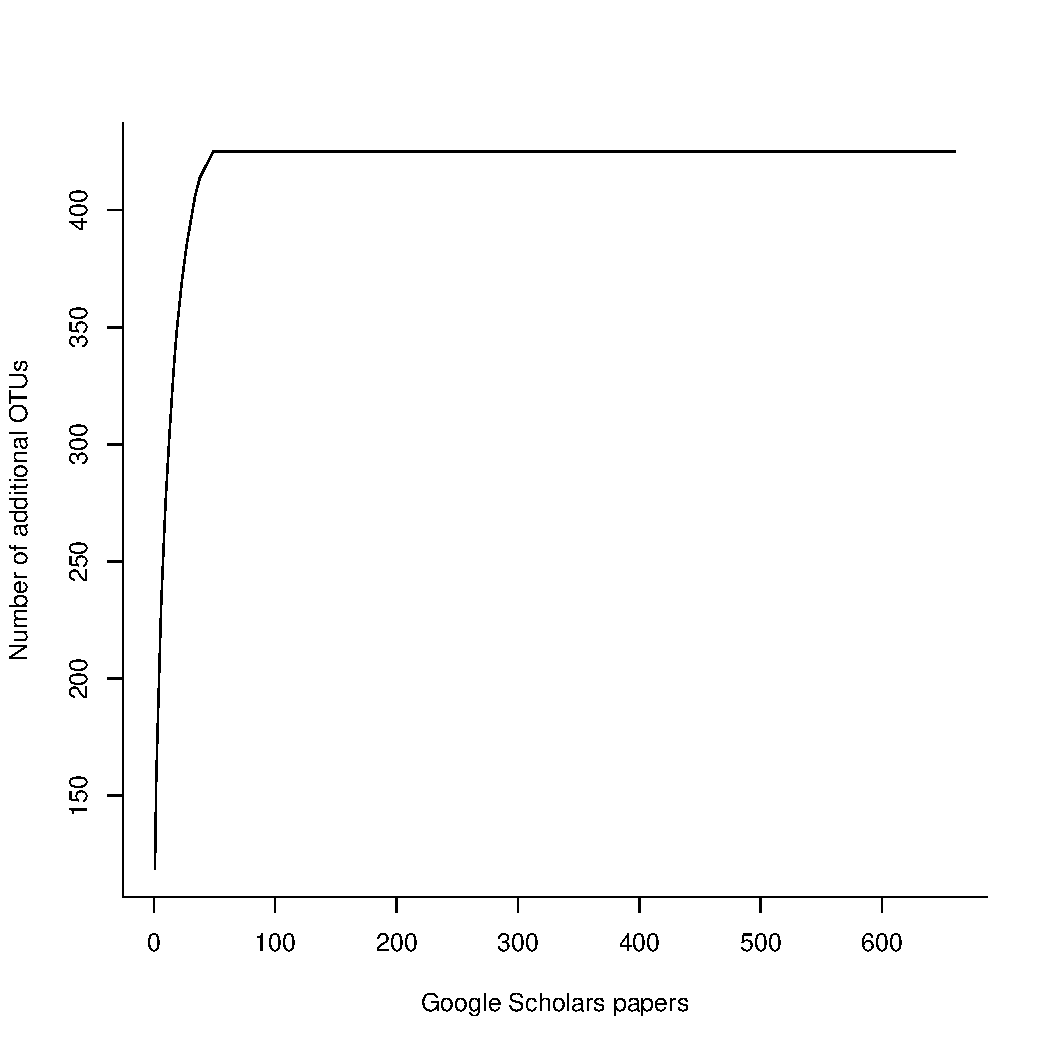
\includegraphics[width=1\textwidth]{Missing_mammals/Figures/Supp_figure_google_searches.pdf}
\caption[Google searches additional OTUs rarefaction curve.]{Google searches additional OTUs rarefaction curve. The x axis represent the number of google scholar matches (papers, books or abstracts) and the y axis represents the cumulative number of additional living OTUs per google scholar match.}
\label{Supp_figure_google_searches}
\end{figure}

We transformed all the non-nexus matrices (tnt, word, excel, jpeg) to nexus format manually.
In total, we downloaded 286 matrices containing a total of 11010 operational taxonomic units (OTUs) of which 5228 were unique.
In this study, we refer to OTUs rather than species since the entries in the downloaded matrices were not standardised and ranged from specific individual specimen names (i.e. the name of a collection item) to the family-level.
Where possible, we considered OTUs at their lowest valid taxonomic level (i.e. species) but some OTUs were only valid at a higher taxonomic level (e.g. genus or family).
Therefore for some orders, we sampled more genera than species (Table \ref{Table_results}).

To select the lowest valid taxonomic level for each OTU, we standardised their taxonomy by correcting species names so they matched standard taxonomic nomenclature (e.g., \textit{H. sapiens} was transformed to \textit{Homo sapiens}).
We designated as ``living'' all OTUs that were either present in the phylogeny of \citep{BinindaEmonds} or the taxonomy of \citep{wilson2005mammal}, and designated as ``fossil'' all OTUs that were present in the Paleobiology database (\url{https://paleobiodb.org/}).

For OTUs that did not appear in these three sources, we first decomposed the name (i.e. \textit{Homo sapiens} became \textit{Homo} and \textit{sapiens}) and tried to match the first element with a higher taxonomic level (genus or family).
Any OTUs that still had no matches in the sources above were designated as non-applicable (NA; see Fig. \ref{Supp_figure_Taxonomic_algorithm}).

\begin{figure}[!h]
\centering
    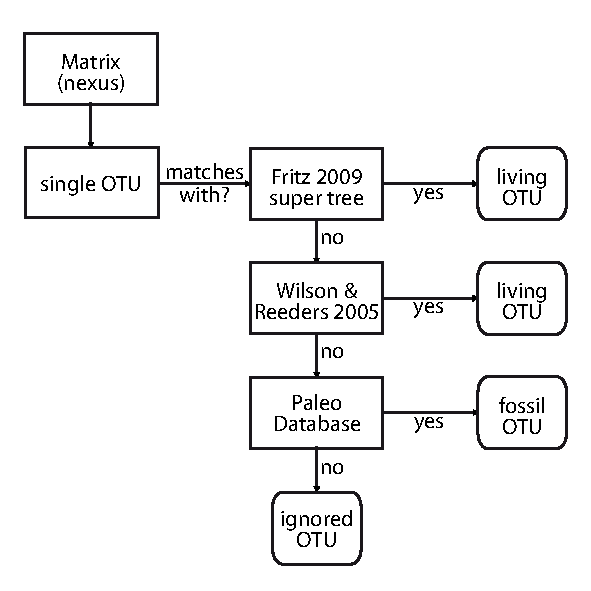
\includegraphics[width=1\textwidth]{Missing_mammals/Figures/Supp_figure_Taxonomic_algorithm.pdf}
\caption[Taxonomic matching algorithm used in this study.]{Taxonomic matching algorithm used in this study. For each matrix, each operational taxonomic units (OTU) is matched with the super tree from Bininda-Emonds 2007. If the OTU matches, then it is classified as living. Else it is matched with the Wilson \& Reeders 2005 taxonomy list. If the OTU matches, then it is classified as living. Else it is matched with the Paleo Database list of mammals. If the OTU matches, then it is classified as fossil. Else it is ignored.}
\label{Supp_figure_Taxonomic_algorithm}
\end{figure}

The number of characters in each matrix ranged from 6 to 4541.
Matrices with few characters are problematic when comparing available data among matrices because (1) they have less chance of having characters that overlap with those of other matrices \citep{wagner2000} and (2) they are more likely to contain a higher proportion of specific characters that are not-applicable across large clades \citep[e.g. ``antler ramifications'' is a character that is only applicable to Cervidae not all mammals][]{Brazeau2011}.
Therefore we selected only matrices containing \textgreater 100 characters for each OTU.
This threshold was chosen to correspond with the number of characters used in \citep{GuillermeCooper} and \citep{harrisonamong-character2014}.
Note that results of analyses with no character threshold are available in Supplementary Material. 
After removing all matrices with \textless 100 characters, we retained 1074 unique living mammal OTUs from 126 matrices for our analyses. % 1601 unique living OTUs for 286 matrices (no threshold)

\subsection{Data availability and distribution}
To assess the availability of cladistic data for each mammalian order, we calculated the percentage of OTUs with cladistic data at three different taxonomic levels: family, genus and species.
%We used these different taxonomic levels because some clades are well covered at the family- or genus-level, but poorly covered at the species-level. % NC: Probably obvious?
We consider orders with \textless 25\% of living taxa with cladistic data as having poor data coverage (``low'' coverage), and orders with \textgreater 75\% of living taxa with cladistic data as having good data coverage (hereafter ``high'' coverage). 

For orders with \textless 100\% cladistic data coverage at any taxonomic level, we investigated whether the available cladistic data was (i) randomly distributed, (ii) overdispersed or (iii) clustered, with respect to phylogeny, using two metrics from community phylogenetics: the Nearest Taxon Index (NTI; \citep{webb2002phylogenies} and the Net Relatedness Index (NRI; \citep{webb2002phylogenies}. 
NTI is most sensitive to clustering or overdispersion near the tips, whereas NRI is more sensitive to clustering or overdispersion across the whole phylogeny \citep{Cooper2008}. 
Both metrics were calculated using the \texttt{picante} package in R \citep{picante,R}.

NTI \citep{webb2002phylogenies} is based on mean nearest neighbour distance (MNND) and is calculated as follows:
  \begin{equation}
    NTI=-\left(\frac{\overline{MNND}_{obs}-\overline{MNND}_{n}}{\sigma(MNND_{n})}\right)
  \end{equation}
where $\overline{MNND}_{obs}$ is the observed mean distance between each of $n$ taxa with cladistic data and its nearest neighbour with cladistic data in the phylogeny, 
$\overline{MNND}_{n}$ is the mean of 1000 mean MNND between $n$ randomly drawn taxa, and $\sigma(MNND_{n})$ is the standard deviation of these 1000 random MNND values.
NRI is similar but is based on mean phylogenetic distance (MPD) as follows:
  \begin{equation}
    NRI=-\left(\frac{\overline{MPD}_{obs}-\overline{MPD}_{n}}{\sigma(MPD_{n})}\right)
  \end{equation}
where $\overline{MPD}_{obs}$ is the observed mean phylogenetic distance of the tree containing only the $n$ taxa with cladistic data, $\overline{MPD}_{n}$ is the expected random MPD for $n$ taxa estimated by calculating the MPD from $n$ taxa randomly drawn from the phylogeny and repeated 1000 times, and $\sigma(MPD_{n})$ is the standard deviation of the 1000 random MPD values. % NC: This can be shortened a bit but it's only gonna save you 50 words max.
Negative NTI and NRI values show that the focal taxa are more overdispersed across the phylogeny than expected by chance, and positive values reflect significant clustering.

We calculated NTI and NRI values for each mammalian order separately, at each different taxonomic level. 
For each analysis our focal taxa were those with available cladistic data at that taxonomic level and the phylogeny was the phylogeny of the order pruned from \citep{BinindaEmonds}.

%---------------------------------------------
%
%       RESULTS
%
%---------------------------------------------

\section{Results}
Across the 126 cladistic matrices we extracted, 22 out of 28 mammalian orders have low coverage (\textless 25\% of species with cladistic data) and six have high coverage (\textgreater 75\% of species with cladistic data) at the species-level.
At the genus-level, three orders have low coverage and 12 have high coverage, and at the family-level, no orders have low coverage and 23 have high coverage (Table \ref{Table_results}).

% latex table generated in R 3.2.0 by xtable 1.7-4 package
% Sun Jun 21 15:26:40 2015
\begin{longtable}{lL{1.8cm}C{2cm}lcc}
\caption{Number of taxa with available cladistic data for mammalian orders at three taxonomic levels. The left vertical bar represents ``low'' coverage (\textless 25\%); the right vertical bar represents ``high'' coverage (\textgreater 75\%). A negative Net Relatedness Index (NRI) and Nearest Taxon Index (NTI) shows more phylogeneticaly dispersed taxa than expected by chance; a positive value shows more phylogeneticaly clustered taxa than expected by chance. Significant NRI or NTI values are highlighted in bold. One star (*) signifies a p-value between 0.05 and 0.005; two starts between 0.005 and 0.0005 and three stars \textless 0.0005.} \\ 
  \hline
Order & Taxonomic level & Proportion of taxa & Coverage & NRI & NTI \\ 
  \hline
Afrosoricida & family & 2/2 & 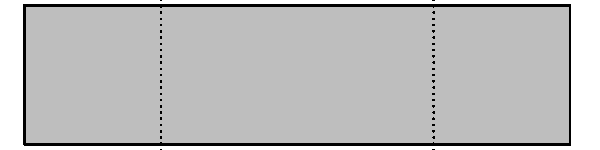
\includegraphics[width=0.20\linewidth, height=0.05\linewidth]{Missing_mammals/Table_figures/bar1.pdf} &   &   \\ 
  Afrosoricida & genus & 17/17 & 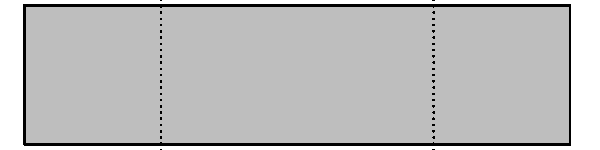
\includegraphics[width=0.20\linewidth, height=0.05\linewidth]{Missing_mammals/Table_figures/bar2.pdf} &   &   \\ 
  \textbf{Afrosoricida} & \textbf{species} & \textbf{23/42} & 
\includegraphics[width=0.20\linewidth, height=0.05\linewidth]{Missing_mammals/Table_figures/bar3.pdf} & \textbf{1.89*} & 1.19 \\ 
  Carnivora & family & 11/15 & 
\includegraphics[width=0.20\linewidth, height=0.05\linewidth]{Missing_mammals/Table_figures/bar4.pdf} & 0.43 & 1.68 \\ 
  \textbf{Carnivora} & \textbf{genus} & \textbf{30/125} & 
\includegraphics[width=0.20\linewidth, height=0.05\linewidth]{Missing_mammals/Table_figures/bar5.pdf} & \textbf{4.14**} & \textbf{1.81*} \\ 
  \textbf{Carnivora} & \textbf{species} & \textbf{42/283} & 
\includegraphics[width=0.20\linewidth, height=0.05\linewidth]{Missing_mammals/Table_figures/bar6.pdf} & \textbf{18.64**} & \textbf{3.02**} \\ 
  Cetartiodactyla & family & 21/21 & 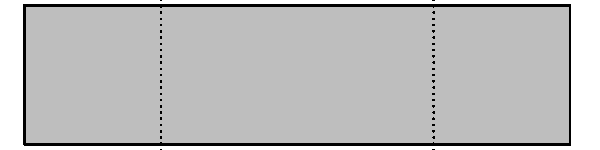
\includegraphics[width=0.20\linewidth, height=0.05\linewidth]{Missing_mammals/Table_figures/bar7.pdf} &   &   \\ 
  \textbf{Cetartiodactyla} & \textbf{genus} & \textbf{77/128} & 
\includegraphics[width=0.20\linewidth, height=0.05\linewidth]{Missing_mammals/Table_figures/bar8.pdf} & 0.87 & \textbf{1.77*} \\ 
  \textbf{Cetartiodactyla} & \textbf{species} & \textbf{129/310} & 
\includegraphics[width=0.20\linewidth, height=0.05\linewidth]{Missing_mammals/Table_figures/bar9.pdf} & \textbf{2.72*} & 0.04 \\ 
  Chiroptera & family & 13/18 & 
\includegraphics[width=0.20\linewidth, height=0.05\linewidth]{Missing_mammals/Table_figures/bar10.pdf} & 0.55 & 0.63 \\ 
  \textbf{Chiroptera} & \textbf{genus} & \textbf{85/202} & 
\includegraphics[width=0.20\linewidth, height=0.05\linewidth]{Missing_mammals/Table_figures/bar11.pdf} & \textbf{16.91**} & \textbf{2.85**} \\ 
  \textbf{Chiroptera} & \textbf{species} & \textbf{165/1053} & 
\includegraphics[width=0.20\linewidth, height=0.05\linewidth]{Missing_mammals/Table_figures/bar12.pdf} & \textbf{14.55**} & \textbf{3.44**} \\ 
  Cingulata & family & 1/1 & 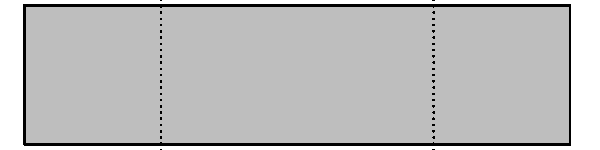
\includegraphics[width=0.20\linewidth, height=0.05\linewidth]{Missing_mammals/Table_figures/bar13.pdf} &   &   \\ 
  Cingulata & genus & 8/9 & 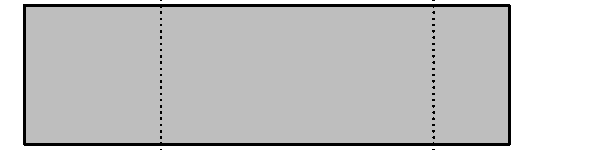
\includegraphics[width=0.20\linewidth, height=0.05\linewidth]{Missing_mammals/Table_figures/bar14.pdf} & 1.49 & -1.63 \\ 
  Cingulata & species & 6/29 & 
\includegraphics[width=0.20\linewidth, height=0.05\linewidth]{Missing_mammals/Table_figures/bar15.pdf} & 1.43 & 0.36 \\ 
  Dasyuromorphia & family & 2/2 & 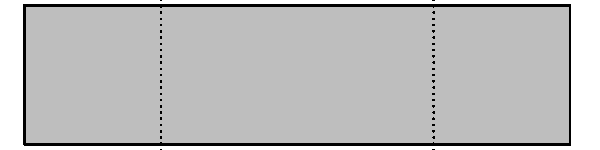
\includegraphics[width=0.20\linewidth, height=0.05\linewidth]{Missing_mammals/Table_figures/bar16.pdf} &   &   \\ 
  Dasyuromorphia & genus & 7/22 & 
\includegraphics[width=0.20\linewidth, height=0.05\linewidth]{Missing_mammals/Table_figures/bar17.pdf} & -1 & -1.45 \\ 
  Dasyuromorphia & species & 8/64 & 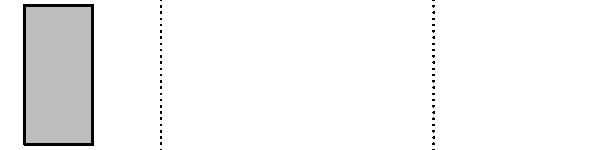
\includegraphics[width=0.20\linewidth, height=0.05\linewidth]{Missing_mammals/Table_figures/bar18.pdf} & -1.15 & -0.62 \\ 
  Dermoptera & family & 1/1 & 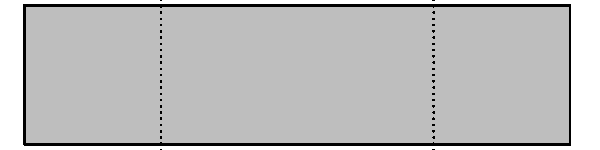
\includegraphics[width=0.20\linewidth, height=0.05\linewidth]{Missing_mammals/Table_figures/bar19.pdf} &   &   \\ 
  Dermoptera & genus & 1/2 & 
\includegraphics[width=0.20\linewidth, height=0.05\linewidth]{Missing_mammals/Table_figures/bar20.pdf} &   &   \\ 
  Dermoptera & species & 1/2 & 
\includegraphics[width=0.20\linewidth, height=0.05\linewidth]{Missing_mammals/Table_figures/bar21.pdf} &   &   \\ 
  Didelphimorphia & family & 1/1 & 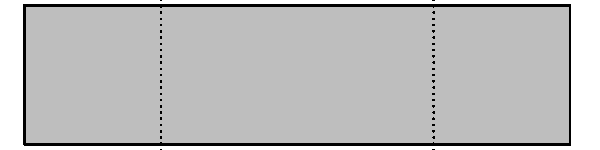
\includegraphics[width=0.20\linewidth, height=0.05\linewidth]{Missing_mammals/Table_figures/bar22.pdf} &   &   \\ 
  Didelphimorphia & genus & 16/16 & 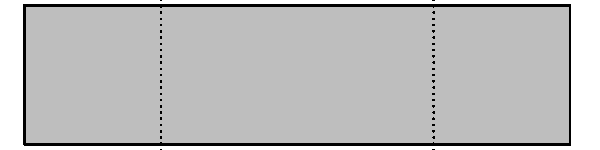
\includegraphics[width=0.20\linewidth, height=0.05\linewidth]{Missing_mammals/Table_figures/bar23.pdf} &   &   \\ 
  Didelphimorphia & species & 40/84 & 
\includegraphics[width=0.20\linewidth, height=0.05\linewidth]{Missing_mammals/Table_figures/bar24.pdf} & -0.94 & 0.36 \\ 
  Diprotodontia & family & 9/11 & 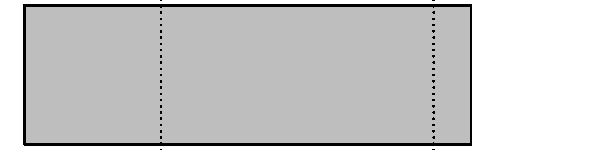
\includegraphics[width=0.20\linewidth, height=0.05\linewidth]{Missing_mammals/Table_figures/bar25.pdf} & -0.8 & 0.56 \\ 
  Diprotodontia & genus & 20/38 & 
\includegraphics[width=0.20\linewidth, height=0.05\linewidth]{Missing_mammals/Table_figures/bar26.pdf} & -1.36 & -0.73 \\ 
  Diprotodontia & species & 16/126 & 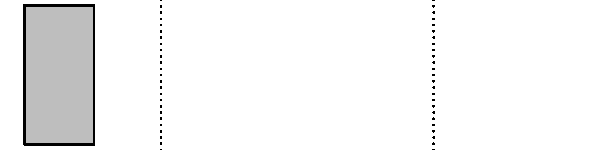
\includegraphics[width=0.20\linewidth, height=0.05\linewidth]{Missing_mammals/Table_figures/bar27.pdf} & -2.29 & -1.55 \\ 
  Erinaceomorpha & family & 1/1 & 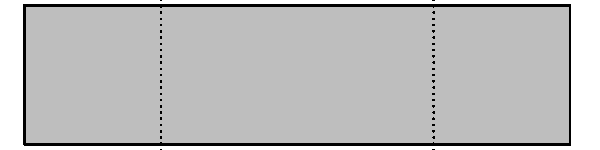
\includegraphics[width=0.20\linewidth, height=0.05\linewidth]{Missing_mammals/Table_figures/bar28.pdf} &   &   \\ 
  Erinaceomorpha & genus & 10/10 & 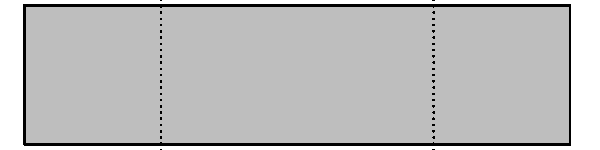
\includegraphics[width=0.20\linewidth, height=0.05\linewidth]{Missing_mammals/Table_figures/bar29.pdf} &   &   \\ 
  Erinaceomorpha & species & 21/22 & 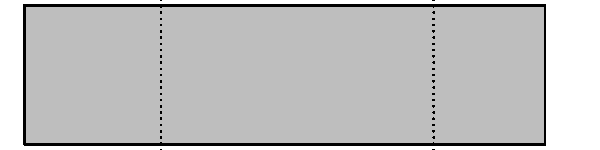
\includegraphics[width=0.20\linewidth, height=0.05\linewidth]{Missing_mammals/Table_figures/bar30.pdf} & -1.1 & -0.3 \\ 
  Hyracoidea & family & 1/1 & 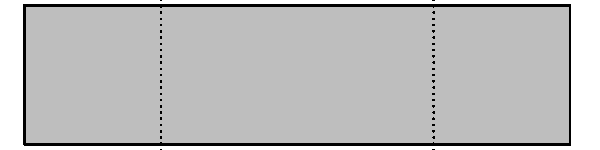
\includegraphics[width=0.20\linewidth, height=0.05\linewidth]{Missing_mammals/Table_figures/bar31.pdf} &   &   \\ 
  Hyracoidea & genus & 1/3 & 
\includegraphics[width=0.20\linewidth, height=0.05\linewidth]{Missing_mammals/Table_figures/bar32.pdf} &   &   \\ 
  Hyracoidea & species & 1/4 & 
\includegraphics[width=0.20\linewidth, height=0.05\linewidth]{Missing_mammals/Table_figures/bar33.pdf} &   &   \\ 
  Lagomorpha & family & 1/2 & 
\includegraphics[width=0.20\linewidth, height=0.05\linewidth]{Missing_mammals/Table_figures/bar34.pdf} &   &   \\ 
  Lagomorpha & genus & 1/12 & 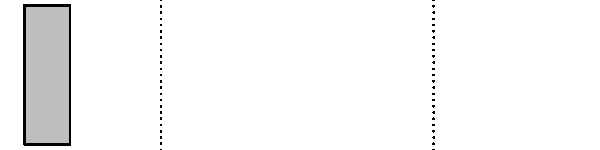
\includegraphics[width=0.20\linewidth, height=0.05\linewidth]{Missing_mammals/Table_figures/bar35.pdf} &   &   \\ 
  Lagomorpha & species & 1/86 & 
\includegraphics[width=0.20\linewidth, height=0.05\linewidth]{Missing_mammals/Table_figures/bar36.pdf} &   &   \\ 
  Macroscelidea & family & 1/1 & 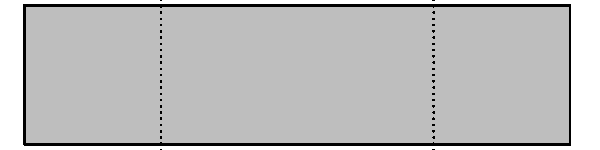
\includegraphics[width=0.20\linewidth, height=0.05\linewidth]{Missing_mammals/Table_figures/bar37.pdf} &   &   \\ 
  Macroscelidea & genus & 4/4 & \includegraphics[width=0.20\linewidth, height=0.05\linewidth]{Missing_mammals/Table_figures/bar38.pdf} &   &   \\ 
  Macroscelidea & species & 5/15 & \includegraphics[width=0.20\linewidth, height=0.05\linewidth]{Missing_mammals/Table_figures/bar39.pdf} & -0.98 & -1.38 \\ 
  Microbiotheria & family & 1/1 & \includegraphics[width=0.20\linewidth, height=0.05\linewidth]{Missing_mammals/Table_figures/bar40.pdf} &   &   \\ 
  Microbiotheria & genus & 1/1 & \includegraphics[width=0.20\linewidth, height=0.05\linewidth]{Missing_mammals/Table_figures/bar41.pdf} &   &   \\ 
  Microbiotheria & species & 1/1 & \includegraphics[width=0.20\linewidth, height=0.05\linewidth]{Missing_mammals/Table_figures/bar42.pdf} &   &   \\ 
  Monotremata & family & 2/2 & \includegraphics[width=0.20\linewidth, height=0.05\linewidth]{Missing_mammals/Table_figures/bar43.pdf} &   &   \\ 
  Monotremata & genus & 2/3 & \includegraphics[width=0.20\linewidth, height=0.05\linewidth]{Missing_mammals/Table_figures/bar44.pdf} & -0.71 & -0.71 \\ 
  Monotremata & species & 2/4 & \includegraphics[width=0.20\linewidth, height=0.05\linewidth]{Missing_mammals/Table_figures/bar45.pdf} & -1.01 & -1.03 \\ 
  Notoryctemorphia & family & 1/1 & \includegraphics[width=0.20\linewidth, height=0.05\linewidth]{Missing_mammals/Table_figures/bar46.pdf} &   &   \\ 
  Notoryctemorphia & genus & 1/1 & \includegraphics[width=0.20\linewidth, height=0.05\linewidth]{Missing_mammals/Table_figures/bar47.pdf} &   &   \\ 
  Notoryctemorphia & species & 0/2 & \includegraphics[width=0.20\linewidth, height=0.05\linewidth]{Missing_mammals/Table_figures/bar48.pdf} &   &   \\ 
  Paucituberculata & family & 1/1 & \includegraphics[width=0.20\linewidth, height=0.05\linewidth]{Missing_mammals/Table_figures/bar49.pdf} &   &   \\ 
  Paucituberculata & genus & 2/3 & \includegraphics[width=0.20\linewidth, height=0.05\linewidth]{Missing_mammals/Table_figures/bar50.pdf} & 0 & 0 \\ 
  Paucituberculata & species & 2/5 & \includegraphics[width=0.20\linewidth, height=0.05\linewidth]{Missing_mammals/Table_figures/bar51.pdf} & -0.64 & -0.65 \\ 
  Peramelemorphia & family & 2/2 & \includegraphics[width=0.20\linewidth, height=0.05\linewidth]{Missing_mammals/Table_figures/bar52.pdf} &   &   \\ 
  Peramelemorphia & genus & 7/7 & \includegraphics[width=0.20\linewidth, height=0.05\linewidth]{Missing_mammals/Table_figures/bar53.pdf} &   &   \\ 
  Peramelemorphia & species & 16/18 & \includegraphics[width=0.20\linewidth, height=0.05\linewidth]{Missing_mammals/Table_figures/bar54.pdf} & -0.09 & 1 \\ 
  Perissodactyla & family & 3/3 & \includegraphics[width=0.20\linewidth, height=0.05\linewidth]{Missing_mammals/Table_figures/bar55.pdf} &   &   \\ 
  Perissodactyla & genus & 6/6 & \includegraphics[width=0.20\linewidth, height=0.05\linewidth]{Missing_mammals/Table_figures/bar56.pdf} &   &   \\ 
  Perissodactyla & species & 7/16 & \includegraphics[width=0.20\linewidth, height=0.05\linewidth]{Missing_mammals/Table_figures/bar57.pdf} & 0.62 & -2.5 \\ 
  Pholidota & family & 1/1 & \includegraphics[width=0.20\linewidth, height=0.05\linewidth]{Missing_mammals/Table_figures/bar58.pdf} &   &   \\ 
  Pholidota & genus & 1/1 & \includegraphics[width=0.20\linewidth, height=0.05\linewidth]{Missing_mammals/Table_figures/bar59.pdf} &   &   \\ 
  \textbf{Pholidota} & \textbf{species} & \textbf{3/8} & \includegraphics[width=0.20\linewidth, height=0.05\linewidth]{Missing_mammals/Table_figures/bar60.pdf} & \textbf{2.64*} & \textbf{2.23*} \\ 
  Pilosa & family & 3/5 & \includegraphics[width=0.20\linewidth, height=0.05\linewidth]{Missing_mammals/Table_figures/bar61.pdf} & 0.94 & 0.93 \\ 
  Pilosa & genus & 3/5 & \includegraphics[width=0.20\linewidth, height=0.05\linewidth]{Missing_mammals/Table_figures/bar62.pdf} & -0.36 & -0.31 \\ 
  Pilosa & species & 3/29 & \includegraphics[width=0.20\linewidth, height=0.05\linewidth]{Missing_mammals/Table_figures/bar63.pdf} & 0.33 & 0.79 \\ 
  Primates & family & 15/15 & \includegraphics[width=0.20\linewidth, height=0.05\linewidth]{Missing_mammals/Table_figures/bar64.pdf} &   &   \\ 
  Primates & genus & 48/68 & \includegraphics[width=0.20\linewidth, height=0.05\linewidth]{Missing_mammals/Table_figures/bar65.pdf} & -0.41 & -1.4 \\ 
  Primates & species & 56/351 & \includegraphics[width=0.20\linewidth, height=0.05\linewidth]{Missing_mammals/Table_figures/bar66.pdf} & -1.6 & -2.04 \\ 
  Proboscidea & family & 1/1 & \includegraphics[width=0.20\linewidth, height=0.05\linewidth]{Missing_mammals/Table_figures/bar67.pdf} &   &   \\ 
  Proboscidea & genus & 1/2 & \includegraphics[width=0.20\linewidth, height=0.05\linewidth]{Missing_mammals/Table_figures/bar68.pdf} &   &   \\ 
  Proboscidea & species & 1/3 & \includegraphics[width=0.20\linewidth, height=0.05\linewidth]{Missing_mammals/Table_figures/bar69.pdf} &   &   \\ 
  Rodentia & family & 11/32 & \includegraphics[width=0.20\linewidth, height=0.05\linewidth]{Missing_mammals/Table_figures/bar70.pdf} & -0.46 & -1.91 \\ 
  Rodentia & genus & 21/450 & \includegraphics[width=0.20\linewidth, height=0.05\linewidth]{Missing_mammals/Table_figures/bar71.pdf} & -2.11 & 0.3 \\ 
  Rodentia & species & 15/2094 & \includegraphics[width=0.20\linewidth, height=0.05\linewidth]{Missing_mammals/Table_figures/bar72.pdf} & -1.65 & -2.55 \\ 
  Scandentia & family & 2/2 & \includegraphics[width=0.20\linewidth, height=0.05\linewidth]{Missing_mammals/Table_figures/bar73.pdf} &   &   \\ 
  Scandentia & genus & 2/5 & \includegraphics[width=0.20\linewidth, height=0.05\linewidth]{Missing_mammals/Table_figures/bar74.pdf} & -0.77 & -0.76 \\ 
  Scandentia & species & 2/20 & \includegraphics[width=0.20\linewidth, height=0.05\linewidth]{Missing_mammals/Table_figures/bar75.pdf} & -1.79 & -1.99 \\ 
  Sirenia & family & 2/2 & \includegraphics[width=0.20\linewidth, height=0.05\linewidth]{Missing_mammals/Table_figures/bar76.pdf} &   &   \\ 
  Sirenia & genus & 2/2 & \includegraphics[width=0.20\linewidth, height=0.05\linewidth]{Missing_mammals/Table_figures/bar77.pdf} &   &   \\ 
  Sirenia & species & 4/4 & \includegraphics[width=0.20\linewidth, height=0.05\linewidth]{Missing_mammals/Table_figures/bar78.pdf} &   &   \\ 
  Soricomorpha & family & 3/4 & \includegraphics[width=0.20\linewidth, height=0.05\linewidth]{Missing_mammals/Table_figures/bar79.pdf} & -0.93 & -0.92 \\ 
  \textbf{Soricomorpha} & \textbf{genus} & \textbf{19/43} & \includegraphics[width=0.20\linewidth, height=0.05\linewidth]{Missing_mammals/Table_figures/bar80.pdf} & \textbf{6.98**} & \textbf{2.49*} \\ 
  \textbf{Soricomorpha} & \textbf{species} & \textbf{19/392} & \includegraphics[width=0.20\linewidth, height=0.05\linewidth]{Missing_mammals/Table_figures/bar81.pdf} & \textbf{13.19**} & \textbf{3.89**} \\ 
  Tubulidentata & family & 1/1 & \includegraphics[width=0.20\linewidth, height=0.05\linewidth]{Missing_mammals/Table_figures/bar82.pdf} &   &   \\ 
  Tubulidentata & genus & 1/1 & \includegraphics[width=0.20\linewidth, height=0.05\linewidth]{Missing_mammals/Table_figures/bar83.pdf} &   &   \\ 
  Tubulidentata & species & 1/1 & \includegraphics[width=0.20\linewidth, height=0.05\linewidth]{Missing_mammals/Table_figures/bar84.pdf} &   &   \\ 
   \hline
\hline
\label{Table_results}
\end{longtable}


Among the mammalian orders containing OTUs with no available cladistic data, only six orders had significantly clustered data (Carnivora, Cetartiodactyla, Chiroptera and Soricomorpha at both species- and genus-level and Afrosoricida and Pholidota at the species-level only) and no order had significantly overdispersed data at any taxonomic level (Table \ref{Table_results}).

Two contrasting results are shown in Fig. \ref{Figure_example_coverage} with randomly distributed OTUs with cladistic data in Primates (Fig. \ref{Figure_example_coverage}A) and phylogenetically clustered OTUs with cladistic data in Carnivora (mainly Canidae; Fig. \ref{Figure_example_coverage}B).

\begin{figure}[!h]
\centering
    \includegraphics[width=1\textwidth]{Missing_mammals/Figures/example_coverage.pdf}
\caption[Phylogenetic distribution of species with available cladistic data across Primates and Carnivora]{Phylogenetic distribution of species with available cladistic data across two mammalian orders (A: Primates; B: Carnivora).
Edges are colored in grey when no cladistic data are available for a species and in blue when data are available.}
\label{Figure_example_coverage}
\end{figure}

%---------------------------------------------
%
%       DISCUSSION
%
%---------------------------------------------

\section{Discussion}
Our results show that although phylogenetic relationships among living mammals are well-resolved \citep[e.g.][]{BinindaEmonds,meredithimpacts2011} , most of the data used to build these phylogenies is molecular, and very little cladistic data are available for living mammals compared to fossil mammals \citep[e.g.][]{O'Leary08022013,ni2013oldest}.
This has implications for building Total Evidence phylogenies containing both living and fossil mammals, as without sufficient cladistic data for living species, fossil placements in these trees are very uncertain \citep{GuillermeCooper}.
Cladistic data coverage in living mammals varies across taxonomic levels and in its phylogenetic distribution.
Higher taxonomic levels are always better sampled than lower ones and within these taxonomic levels, the available data are mostly randomly distributed across the phylogeny, apart from in six orders).

The number of living mammalian taxa with no available cladistic data was surprisingly high at the species-level: only six out of 28 orders have a high coverage of taxa with available cladistic data (and two of the 28 orders are monospecific!).
This high coverage threshold of 75\% of taxa with available cladistic data represents the minimum amount of data required before missing data has a significant effect on the topology of Total Evidence trees \citep{GuillermeCooper}.
Beyond this threshold, there is considerable displacement of wildcard taxa \citep[\textit{sensu}][]{kearneyfragmentary2002} and decreases in clade conservation \citep{GuillermeCooper}.
Therefore we expect a high probability of topological artefacts for the placement of fossil taxa at the species-level in most mammalian orders.
However, data coverage seems to be less of an issue at higher taxonomic levels (i.e. genus- and family-level).
This point is important from a practical point of view because of the slight discrepancy between the neontological and palaeontological concept of species.
While neontological species are described using morphology, genetic distance, spatial distribution and even behaviour, palaeontological species can be based only on morphological, spatial and temporal data \citep[e.g.][]{ni2013oldest}.
Because of this, most palaeontological studies are using the genus as their smallest OTU \citep[e.g.][]{ni2013oldest,O'Leary08022013}.
Thus data availability at the genus-level in living mammals should be our primary concern when aiming to build phylogenies of living and fossil taxa.

When only a few species with cladistic data are available, the ideal scenario is for them to be phylogenetically overdispersed (i.e. that there is data for at least every sub-clade) to maximize the possibilities of a fossil branching from the right clade.
The second best scenario is that species with cladistic data are randomly distributed across the phylogeny. 
In this scenario we expect no special bias in the placement of the fossil \citep{GuillermeCooper}, it is therefore encouraging that for most orders, species with cladistic data were randomly distributed across the phylogeny of each order.
The worst case scenario for fossil placement is that species with cladistic data are phylogenetically clustered. 
In this situation we expect two major biases to occur: first, the fossil will not be able to branch within a clade containing no data, and second, the fossil will have a higher probability, at random, of branching within the clade containing most of the available data.
This means that fossils with uncertain phylogenetic affinities (\textit{incertae sedis} will have a higher probability of branching within the most sampled clade just by chance).
Our results suggest that this may be an issue, at the genus-level, in Carnivora, Cetartiodactyla, Chiroptera and Soricomorpha. 
For example, a Carnivora fossil will be unable to branch in the Herpestidae that has no species with cladistic data, and will also have more chance to branch, randomly, within the Canidae clade than any other clade in Carnivora (Fig. \ref{Figure_example_coverage}B).
Thus, in Total Evidence trees, placements of some carnivoran fossils should considered with caution. 
% NC: Trying not to piss off GraHam - really it's weird stuff appearing in Carnivora that we are concerned by, not all Carnivora. TG: I think it's mainly Graham's work that focuses on canids.
In this study, we treated all cladistic matrices as equal in a similar way to molecular matrices. 
For example, if matrix A contained 100 characters for taxa X and Y, and matrix B contained 50 different characters for taxa X and Z, we assumed that both matrices can be combined in a supermatrix containing 150 independent characters for taxon X, 100 for taxon Y and 50 for taxon Z.
Unfortunately, cladistic data cannot always be treated in this way because some characters may overlap.
For example, if matrix A has a character coding for the shape of a particular morphological feature and matrix B has a character coding for the presence of this same morphological feature and a second character coding for its shape, then these three characters are non-independent compound characters \citep{Brazeau2011}.
However, in reasonably sized matrices \citep[\textgreater 100 characters;][]{GuillermeCooper,harrisonamong-character2014} it is more likely that a number of characters are consistently conserved among the different matrices and thus easily combinable.
For example, within the Primate cladistic literature, the character \textit{p7} - the size of the $4^{th}$ lower premolar paraconid - has been used consistently for \textgreater 15 years \citep[e.g.][]{ross1998phylogenetic,marivaux2005anthropoid,ni2013oldest} and can therefore be combined among the matrices.
A conservative approach to avoid compound characters would be to select only the most recent matrix for each group, but this would result in the loss of a lot of data.

Despite the absence of good cladistic data coverage for living mammals, the Total Evidence methods still seems to be the most promising way of combining living and fossil data for macroevolutionary analyses. 
Following the recommendations in \citep{GuillermeCooper}, we need to code cladistic characters for as many living species possible. 
Fortunately, data for living mammals is usually readily available in natural history collections, therefore, we propose that an increased effort be put into coding morphological characters from living species, possibly by engaging in collaborative data collection projects through web portals such as \textit{MorphoBank} \citep{morphobank}.
% NC: Still feels like it needs one final sentence to round it all off. Many something like below, but less crappy:
Such an effort would be valuable not only to phylogeneticists, but also to any researcher focusing understanding macroevolutionary patterns and processes.%interested in the diversity of life on Earth.

%Biology letters various stuff

% \bibliographystyle{sysbio}
% \bibliography{References}

%\section{SOM}
%\newcommand{\beginsupplement}{%
%    \setcounter{table}{0}
%    \renewcommand{\thetable}{S\arabic{table}}%
%    \setcounter{figure}{0}
%    \renewcommand{\thefigure}{S\arabic{figure}}%
%}
%\beginsupplement
%
\noindent{\Large \bf Supplementary Material}

\begin{figure}[!htbp]
\centering
    \includegraphics[width=1\textwidth]{Missing_mammals/Supplementary/MissingDataFigure.pdf}
\caption{Example of topological errors due to missing morphological data in living taxa.
The phylogeny contains two clades, Aves and Mammalia, with molecular data (grey) for both but only morphological data (red) for Aves.
If a mammalian fossil species (with no molecular data) is added to the phylogeny, it will erroneously branch with the Aves instead of the Mammalia because no morphological data will overlap between the fossil mammals and the living ones.}
\label{Figure_missing_data_problem}
\end{figure}

\bigskip

\section{Data collection}
1- Data collection: key words, clade (ordinal) metacharacters, Google Search terms, Google Search protocol, Google Search rarefaction curve.

\subsection{Public repositories}
We downloaded available matrices containing fossil and/or living mammal taxa from the three following data bases using the following list of keywords:

\texttt{Mammalia; Monotremata; Marsupialia; Placentalia; Macroscelidea; Afrosoricida; Tubulidentata; Hyracoidea; Proboscidea; Sirenia; Pilosa; Cingulata; Scandentia; Dermoptera; Primates; Lagomorpha; Rodentia; Erinaceomorpha; Soricomorpha; Cetacea; Artiodactyla; Cetartiodactyla; Chiroptera; Perissodactyla; Pholidota; Carnivora; Didelphimorphia; Paucituberculata; Microbiotheria; Dasyuromorphia; Peramelemorphia; Notoryctemorphia; Diprotodontia}.

Details about each public repository specific search option is listed below. Note that some matrices have been downloaded from more than one database but that it is not an issue since we are interested in the total number of living OTUs and that if some where present in more than one matrix, they still only counted as a unique OTU.

\subsubsection{Morphobank}
We accessed the Morphobank repository (\texttt{http://www.morphobank.org/}) on the 5th of December 2014 and used the keywords listed above in the search menue. We downloaded the data associated with each project matching with the keyword.

\subsubsection{Graeme Lloyd}
We accessed Graeme Lloyd's website repository (\texttt{http://graemetlloyd.com/}) on the 5th of December 2014 and downloaded all the matrices that were available with a direct download link in the mammal data section of the website (\texttt{http://graemetlloyd.com/matrmamm.html}).

\subsubsection{Ross Mounce}
We accessed Ross Mounce's GitHub repository (\texttt{https://github.com/rossmounce}) on the 2nd of December 2014 and downloaded every 601 matrix. We then ran a shell script to select only the matrices that had any text element that match with one of the search terms. To make the matrix selection more thorough, we ignored the keywords case as well as the latin suffix (\textit{ia}, \textit{ata}, \textit{ea}, and \textit{a}).

\subsection{Google scholars}
To make sure we didn't miss any extra matrix that wasn't available on one of these repository, we ran a Google Scholar search on the 5th of January. 
We downloaded the additional cladistic matrices from the 20 first search results matching with our selected keywords and with any of the 35 taxonomic levels (mammals Orders, Infraclasses and Class).
We used the following key words:

\texttt{\textit{order} ("morphology" OR "morphological" OR "cladistic") AND characters matrix paleontology phylogeny}

were \textit{order} was replaced by all the keywords listed above. For each 33 keywords, we selected the 20 first papers to match the Google search published since 2010 resulting in 660 papers. Among these papers, not all contained relevant data (discrete morphological characters AND mammalian data). We selected only the 20 first results per search term to avoid downloading articles that were to irrelevant. Among the 660 papers, only 50 contained a total of 425 extra living OTUs (figure ~\ref{Supp_figure_google_searches}).
Also we decided to select only the articles published since 2010 because nearly every one of the recent published matrix contains both a fraction of morphological characters and OTUs from previous studies. For example in primates the character \textit{p7} coded first by \cite{ross1998phylogenetic} is reused with the same living species in \cite{seiffert2003fossil}, \cite{marivaux2005anthropoid}, \cite{seiffert2005basal}, \cite{bloch2007new}, \cite{bloch2007new}, \cite{kay2008anatomy}, \cite{silcox2008biogeographic}, \cite{seiffert2009convergent}, \cite{tabuce2009anthropoid}, \cite{boyer2010astragalar}, \cite{seiffert2010fossil}, \cite{marivaux2013djebelemur} and \cite{ni2013oldest}.

\begin{figure}[!htbp]
\centering
    \includegraphics[width=1\textwidth]{Missing_mammals/Supplementary/Supp_figure_google_searches.pdf}
\caption{Google searches additional OTUs rarefaction curve. The x axis represent the number of google scholar matches (papers, books or abstracts) and the y axis represents the cumulative number of additional living OTUs per google scholar match.}
\label{Supp_figure_google_searches}
\end{figure}

\subsection{Standardising the matrices}
We transformed all the non-nexus matrices (tnt, word, excel, jpeg) to nexus format manually. We then cleaned the nexus matrices by removing any extra information (trees, continuous characters, morphological characters description, molecular data) to end up with nexus matrices containing only the discrete morphological data. We then manually fixed the wrong bionomial names format (e.g. \textit{H. sapiens}) into the correct ones (e.g. \textit{Homo sapiens}) using the abbreviation list in the concerned publications. 

\subsection{Selecting the living OTUs}
Finally we applied a taxonomic matching algorithm to classify the OTUs as either living or fossil. The algorithm is matching every OTU name from every matrix with one of the following taxonomic references: the list of taxa from the Fritz \textit{et al.} supertree (2009) \cite{FritzTree}; the taxonomic list from the Wilson and Reeder's Mammals Species of the World (2005) \cite{wilson2005mammal} and the list of all the mammal fossil from the Paleobio Database (\texttt{http://paleobiodb.org/cgi-bin/bridge.pl?a=login}) accessed on the 13th of Janurary 2015. The OTUs that matched with one of the two first references were considered as living OTUs, the OTUs matching with the third reference were considered as fossil OTUs, finally, the OTUs matching with non of the references were discarded (figure ~\ref{Supp_figure_Taxonomic_algorithm}).

\begin{figure}[!htbp]
\centering
    \includegraphics[width=1\textwidth]{Missing_mammals/Supplementary/Supp_figure_Taxonomic_algorithm.pdf}
\caption{Taxonomic matching algorithm used in this study. For each matrix, each operational taxonomic units (OTU) is matched with the super tree from Fritz 2009. If the OTU matches, then it is classified as living. Else it is matched with the Wilson \& Reeders 2005 taxonomy list. If the OTU matches, then it is classified as living. Else it is matched with the Paleo Database list of mammals. If the OTU matches, then it is classified as fossil. Else it is ignored.}
\label{Supp_figure_Taxonomic_algorithm}
\end{figure}

%\bibliographystyle{vancouver}
%\bibliography{Supp_References}

\section{Supplementary results}
The following section contains supplementary results to the main body: the available data structure using the NTI and the PD metric; the proportion of available data and the data structure for all the matrices (including the matrices with less than 100 characters); and phylogenetical representation of the data availability per order (excluding Primates and Carnivora, present in the main body).

% latex table generated in R 3.2.0 by xtable 1.7-4 package
% Sat Jun 20 17:19:07 2015
\begin{longtable}{lL{1.8cm}C{2cm}lcc}
\caption{Number of taxa with available cladistic data for mammalian orders at three taxonomic levels (without any character threshold; results from the 286 matrices). The coverage represents the proportion of taxa with available morphological data. The left vertical bar represents 25\% of available data (``low'' coverage if \textless 25\%); The right vertical bar represents 75\% of available data (``high'' coverage if \textgreater 75\%). When the Net Relatedness Index (NRI) and the Nearest Taxon Index (NTI) are negative, taxa are more phylogenetically dispersed than expected by chance; when NRI or NTI are positive, taxa are more phylogenetically clustered by expected by chance. Significant NRI or NTI are highlighted in bold. One star (*) represents a p-value between 0.05 and 0.005; two starts between 0.005 and 0.0005 and three stars a p-value less than 0.0005.} \\ 
  \hline
Order & Taxonomic level & Proportion of taxa & Coverage & NRI & NTI \\ 
  \hline
Afrosoricida & family & 2/2 & \includegraphics[width=0.20\linewidth, height=0.05\linewidth]{Missing_mammals/Supplementary/Results_1c/Table_figures/bar1.pdf} &   &   \\ 
  Afrosoricida & genus & 17/17 & \includegraphics[width=0.20\linewidth, height=0.05\linewidth]{Missing_mammals/Supplementary/Results_1c/Table_figures/bar2.pdf} &   &   \\ 
  Afrosoricida & species & 23/42 & \includegraphics[width=0.20\linewidth, height=0.05\linewidth]{Missing_mammals/Supplementary/Results_1c/Table_figures/bar3.pdf} & 1.75 & 1.08 \\ 
  Carnivora & family & 14/15 & \includegraphics[width=0.20\linewidth, height=0.05\linewidth]{Missing_mammals/Supplementary/Results_1c/Table_figures/bar4.pdf} & 0.63 & 0.6 \\ 
  \textbf{Carnivora} & \textbf{genus} & \textbf{54/125} & \includegraphics[width=0.20\linewidth, height=0.05\linewidth]{Missing_mammals/Supplementary/Results_1c/Table_figures/bar5.pdf} & \textbf{4.81**} & \textbf{1.78*} \\ 
  \textbf{Carnivora} & \textbf{species} & \textbf{76/283} & \includegraphics[width=0.20\linewidth, height=0.05\linewidth]{Missing_mammals/Supplementary/Results_1c/Table_figures/bar6.pdf} & \textbf{7.66**} & \textbf{0.85} \\ 
  Cetartiodactyla & family & 21/21 & \includegraphics[width=0.20\linewidth, height=0.05\linewidth]{Missing_mammals/Supplementary/Results_1c/Table_figures/bar7.pdf} &   &   \\ 
  Cetartiodactyla & genus & 100/128 & \includegraphics[width=0.20\linewidth, height=0.05\linewidth]{Missing_mammals/Supplementary/Results_1c/Table_figures/bar8.pdf} & 0.85 & 0.94 \\ 
  \textbf{Cetartiodactyla} & \textbf{species} & \textbf{171/310} & \includegraphics[width=0.20\linewidth, height=0.05\linewidth]{Missing_mammals/Supplementary/Results_1c/Table_figures/bar9.pdf} & \textbf{1.92*} & \textbf{-0.46} \\ 
  Chiroptera & family & 15/18 & \includegraphics[width=0.20\linewidth, height=0.05\linewidth]{Missing_mammals/Supplementary/Results_1c/Table_figures/bar10.pdf} & -0.28 & 0.56 \\ 
  \textbf{Chiroptera} & \textbf{genus} & \textbf{93/202} & \includegraphics[width=0.20\linewidth, height=0.05\linewidth]{Missing_mammals/Supplementary/Results_1c/Table_figures/bar11.pdf} & \textbf{13.47**} & \textbf{1.1} \\ 
  \textbf{Chiroptera} & \textbf{species} & \textbf{215/1053} & \includegraphics[width=0.20\linewidth, height=0.05\linewidth]{Missing_mammals/Supplementary/Results_1c/Table_figures/bar12.pdf} & \textbf{8.82**} & \textbf{1.22} \\ 
  Cingulata & family & 1/1 & \includegraphics[width=0.20\linewidth, height=0.05\linewidth]{Missing_mammals/Supplementary/Results_1c/Table_figures/bar13.pdf} &   &   \\ 
  Cingulata & genus & 8/9 & \includegraphics[width=0.20\linewidth, height=0.05\linewidth]{Missing_mammals/Supplementary/Results_1c/Table_figures/bar14.pdf} & 1.51 & -1.57 \\ 
  \textbf{Cingulata} & \textbf{species} & \textbf{9/29} & \includegraphics[width=0.20\linewidth, height=0.05\linewidth]{Missing_mammals/Supplementary/Results_1c/Table_figures/bar15.pdf} & \textbf{1.9*} & \textbf{0.11} \\ 
  Dasyuromorphia & family & 2/2 & \includegraphics[width=0.20\linewidth, height=0.05\linewidth]{Missing_mammals/Supplementary/Results_1c/Table_figures/bar16.pdf} &   &   \\ 
  Dasyuromorphia & genus & 8/22 & \includegraphics[width=0.20\linewidth, height=0.05\linewidth]{Missing_mammals/Supplementary/Results_1c/Table_figures/bar17.pdf} & -0.75 & -1.07 \\ 
  Dasyuromorphia & species & 9/64 & \includegraphics[width=0.20\linewidth, height=0.05\linewidth]{Missing_mammals/Supplementary/Results_1c/Table_figures/bar18.pdf} & -0.88 & -0.34 \\ 
  Dermoptera & family & 1/1 & \includegraphics[width=0.20\linewidth, height=0.05\linewidth]{Missing_mammals/Supplementary/Results_1c/Table_figures/bar19.pdf} &   &   \\ 
  Dermoptera & genus & 1/2 & \includegraphics[width=0.20\linewidth, height=0.05\linewidth]{Missing_mammals/Supplementary/Results_1c/Table_figures/bar20.pdf} &   &   \\ 
  Dermoptera & species & 1/2 & \includegraphics[width=0.20\linewidth, height=0.05\linewidth]{Missing_mammals/Supplementary/Results_1c/Table_figures/bar21.pdf} &   &   \\ 
  Didelphimorphia & family & 1/1 & \includegraphics[width=0.20\linewidth, height=0.05\linewidth]{Missing_mammals/Supplementary/Results_1c/Table_figures/bar22.pdf} &   &   \\ 
  Didelphimorphia & genus & 16/16 & \includegraphics[width=0.20\linewidth, height=0.05\linewidth]{Missing_mammals/Supplementary/Results_1c/Table_figures/bar23.pdf} &   &   \\ 
  Didelphimorphia & species & 42/84 & \includegraphics[width=0.20\linewidth, height=0.05\linewidth]{Missing_mammals/Supplementary/Results_1c/Table_figures/bar24.pdf} & -1.65 & 0.2 \\ 
  Diprotodontia & family & 11/11 & \includegraphics[width=0.20\linewidth, height=0.05\linewidth]{Missing_mammals/Supplementary/Results_1c/Table_figures/bar25.pdf} &   &   \\ 
  Diprotodontia & genus & 25/38 & \includegraphics[width=0.20\linewidth, height=0.05\linewidth]{Missing_mammals/Supplementary/Results_1c/Table_figures/bar26.pdf} & -1.13 & -1.31 \\ 
  Diprotodontia & species & 31/126 & \includegraphics[width=0.20\linewidth, height=0.05\linewidth]{Missing_mammals/Supplementary/Results_1c/Table_figures/bar27.pdf} & 0.48 & -1.77 \\ 
  Erinaceomorpha & family & 1/1 & \includegraphics[width=0.20\linewidth, height=0.05\linewidth]{Missing_mammals/Supplementary/Results_1c/Table_figures/bar28.pdf} &   &   \\ 
  Erinaceomorpha & genus & 10/10 & \includegraphics[width=0.20\linewidth, height=0.05\linewidth]{Missing_mammals/Supplementary/Results_1c/Table_figures/bar29.pdf} &   &   \\ 
  Erinaceomorpha & species & 21/22 & \includegraphics[width=0.20\linewidth, height=0.05\linewidth]{Missing_mammals/Supplementary/Results_1c/Table_figures/bar30.pdf} & -1.07 & -0.2 \\ 
  Hyracoidea & family & 1/1 & \includegraphics[width=0.20\linewidth, height=0.05\linewidth]{Missing_mammals/Supplementary/Results_1c/Table_figures/bar31.pdf} &   &   \\ 
  Hyracoidea & genus & 1/3 & \includegraphics[width=0.20\linewidth, height=0.05\linewidth]{Missing_mammals/Supplementary/Results_1c/Table_figures/bar32.pdf} &   &   \\ 
  Hyracoidea & species & 1/4 & \includegraphics[width=0.20\linewidth, height=0.05\linewidth]{Missing_mammals/Supplementary/Results_1c/Table_figures/bar33.pdf} &   &   \\ 
  Lagomorpha & family & 2/2 & \includegraphics[width=0.20\linewidth, height=0.05\linewidth]{Missing_mammals/Supplementary/Results_1c/Table_figures/bar34.pdf} &   &   \\ 
  Lagomorpha & genus & 5/12 & \includegraphics[width=0.20\linewidth, height=0.05\linewidth]{Missing_mammals/Supplementary/Results_1c/Table_figures/bar35.pdf} & -1.06 & -0.95 \\ 
  Lagomorpha & species & 12/86 & \includegraphics[width=0.20\linewidth, height=0.05\linewidth]{Missing_mammals/Supplementary/Results_1c/Table_figures/bar36.pdf} & -0.62 & -1.88 \\ 
  Macroscelidea & family & 1/1 & \includegraphics[width=0.20\linewidth, height=0.05\linewidth]{Missing_mammals/Supplementary/Results_1c/Table_figures/bar37.pdf} &   &   \\ 
  Macroscelidea & genus & 4/4 & \includegraphics[width=0.20\linewidth, height=0.05\linewidth]{Missing_mammals/Supplementary/Results_1c/Table_figures/bar38.pdf} &   &   \\ 
  Macroscelidea & species & 12/15 & \includegraphics[width=0.20\linewidth, height=0.05\linewidth]{Missing_mammals/Supplementary/Results_1c/Table_figures/bar39.pdf} & -1.3 & -1.06 \\ 
  Microbiotheria & family & 1/1 & \includegraphics[width=0.20\linewidth, height=0.05\linewidth]{Missing_mammals/Supplementary/Results_1c/Table_figures/bar40.pdf} &   &   \\ 
  Microbiotheria & genus & 1/1 & \includegraphics[width=0.20\linewidth, height=0.05\linewidth]{Missing_mammals/Supplementary/Results_1c/Table_figures/bar41.pdf} &   &   \\ 
  Microbiotheria & species & 1/1 & \includegraphics[width=0.20\linewidth, height=0.05\linewidth]{Missing_mammals/Supplementary/Results_1c/Table_figures/bar42.pdf} &   &   \\ 
  Monotremata & family & 2/2 & \includegraphics[width=0.20\linewidth, height=0.05\linewidth]{Missing_mammals/Supplementary/Results_1c/Table_figures/bar43.pdf} &   &   \\ 
  Monotremata & genus & 2/3 & \includegraphics[width=0.20\linewidth, height=0.05\linewidth]{Missing_mammals/Supplementary/Results_1c/Table_figures/bar44.pdf} & -0.72 & -0.69 \\ 
  Monotremata & species & 2/4 & \includegraphics[width=0.20\linewidth, height=0.05\linewidth]{Missing_mammals/Supplementary/Results_1c/Table_figures/bar45.pdf} & -0.97 & -0.97 \\ 
  Notoryctemorphia & family & 1/1 & \includegraphics[width=0.20\linewidth, height=0.05\linewidth]{Missing_mammals/Supplementary/Results_1c/Table_figures/bar46.pdf} &   &   \\ 
  Notoryctemorphia & genus & 1/1 & \includegraphics[width=0.20\linewidth, height=0.05\linewidth]{Missing_mammals/Supplementary/Results_1c/Table_figures/bar47.pdf} &   &   \\ 
  Notoryctemorphia & species & 0/2 & \includegraphics[width=0.20\linewidth, height=0.05\linewidth]{Missing_mammals/Supplementary/Results_1c/Table_figures/bar48.pdf} &   &   \\ 
  Paucituberculata & family & 1/1 & \includegraphics[width=0.20\linewidth, height=0.05\linewidth]{Missing_mammals/Supplementary/Results_1c/Table_figures/bar49.pdf} &   &   \\ 
  Paucituberculata & genus & 3/3 & \includegraphics[width=0.20\linewidth, height=0.05\linewidth]{Missing_mammals/Supplementary/Results_1c/Table_figures/bar50.pdf} &   &   \\ 
  Paucituberculata & species & 5/5 & \includegraphics[width=0.20\linewidth, height=0.05\linewidth]{Missing_mammals/Supplementary/Results_1c/Table_figures/bar51.pdf} &   &   \\ 
  Peramelemorphia & family & 2/2 & \includegraphics[width=0.20\linewidth, height=0.05\linewidth]{Missing_mammals/Supplementary/Results_1c/Table_figures/bar52.pdf} &   &   \\ 
  Peramelemorphia & genus & 7/7 & \includegraphics[width=0.20\linewidth, height=0.05\linewidth]{Missing_mammals/Supplementary/Results_1c/Table_figures/bar53.pdf} &   &   \\ 
  Peramelemorphia & species & 16/18 & \includegraphics[width=0.20\linewidth, height=0.05\linewidth]{Missing_mammals/Supplementary/Results_1c/Table_figures/bar54.pdf} & -0.13 & 0.97 \\ 
  Perissodactyla & family & 3/3 & \includegraphics[width=0.20\linewidth, height=0.05\linewidth]{Missing_mammals/Supplementary/Results_1c/Table_figures/bar55.pdf} &   &   \\ 
  Perissodactyla & genus & 6/6 & \includegraphics[width=0.20\linewidth, height=0.05\linewidth]{Missing_mammals/Supplementary/Results_1c/Table_figures/bar56.pdf} &   &   \\ 
  Perissodactyla & species & 10/16 & \includegraphics[width=0.20\linewidth, height=0.05\linewidth]{Missing_mammals/Supplementary/Results_1c/Table_figures/bar57.pdf} & -0.07 & -2.63 \\ 
  Pholidota & family & 1/1 & \includegraphics[width=0.20\linewidth, height=0.05\linewidth]{Missing_mammals/Supplementary/Results_1c/Table_figures/bar58.pdf} &   &   \\ 
  Pholidota & genus & 1/1 & \includegraphics[width=0.20\linewidth, height=0.05\linewidth]{Missing_mammals/Supplementary/Results_1c/Table_figures/bar59.pdf} &   &   \\ 
  Pholidota & species & 4/8 & \includegraphics[width=0.20\linewidth, height=0.05\linewidth]{Missing_mammals/Supplementary/Results_1c/Table_figures/bar60.pdf} & 1.18 & 0.94 \\ 
  Pilosa & family & 4/5 & \includegraphics[width=0.20\linewidth, height=0.05\linewidth]{Missing_mammals/Supplementary/Results_1c/Table_figures/bar61.pdf} & 1.87 & 2 \\ 
  Pilosa & genus & 4/5 & \includegraphics[width=0.20\linewidth, height=0.05\linewidth]{Missing_mammals/Supplementary/Results_1c/Table_figures/bar62.pdf} & -0.96 & 0.36 \\ 
  \textbf{Pilosa} & \textbf{species} & \textbf{5/29} & \includegraphics[width=0.20\linewidth, height=0.05\linewidth]{Missing_mammals/Supplementary/Results_1c/Table_figures/bar63.pdf} & \textbf{1.28} & \textbf{2.38*} \\ 
  Primates & family & 15/15 & \includegraphics[width=0.20\linewidth, height=0.05\linewidth]{Missing_mammals/Supplementary/Results_1c/Table_figures/bar64.pdf} &   &   \\ 
  Primates & genus & 48/68 & \includegraphics[width=0.20\linewidth, height=0.05\linewidth]{Missing_mammals/Supplementary/Results_1c/Table_figures/bar65.pdf} & -0.35 & -1.33 \\ 
  Primates & species & 64/351 & \includegraphics[width=0.20\linewidth, height=0.05\linewidth]{Missing_mammals/Supplementary/Results_1c/Table_figures/bar66.pdf} & -0.67 & -1.27 \\ 
  Proboscidea & family & 1/1 & \includegraphics[width=0.20\linewidth, height=0.05\linewidth]{Missing_mammals/Supplementary/Results_1c/Table_figures/bar67.pdf} &   &   \\ 
  Proboscidea & genus & 2/2 & \includegraphics[width=0.20\linewidth, height=0.05\linewidth]{Missing_mammals/Supplementary/Results_1c/Table_figures/bar68.pdf} &   &   \\ 
  Proboscidea & species & 2/3 & \includegraphics[width=0.20\linewidth, height=0.05\linewidth]{Missing_mammals/Supplementary/Results_1c/Table_figures/bar69.pdf} & -0.69 & -0.69 \\ 
  Rodentia & family & 18/32 & \includegraphics[width=0.20\linewidth, height=0.05\linewidth]{Missing_mammals/Supplementary/Results_1c/Table_figures/bar70.pdf} & 0.66 & -0.98 \\ 
  Rodentia & genus & 82/450 & \includegraphics[width=0.20\linewidth, height=0.05\linewidth]{Missing_mammals/Supplementary/Results_1c/Table_figures/bar71.pdf} & -1.66 & 1.55 \\ 
  \textbf{Rodentia} & \textbf{species} & \textbf{90/2094} & \includegraphics[width=0.20\linewidth, height=0.05\linewidth]{Missing_mammals/Supplementary/Results_1c/Table_figures/bar72.pdf} & \textbf{2.76*} & \textbf{2.34*} \\ 
  Scandentia & family & 2/2 & \includegraphics[width=0.20\linewidth, height=0.05\linewidth]{Missing_mammals/Supplementary/Results_1c/Table_figures/bar73.pdf} &   &   \\ 
  Scandentia & genus & 2/5 & \includegraphics[width=0.20\linewidth, height=0.05\linewidth]{Missing_mammals/Supplementary/Results_1c/Table_figures/bar74.pdf} & -0.74 & -0.74 \\ 
  Scandentia & species & 3/20 & \includegraphics[width=0.20\linewidth, height=0.05\linewidth]{Missing_mammals/Supplementary/Results_1c/Table_figures/bar75.pdf} & -1.88 & -0.84 \\ 
  Sirenia & family & 2/2 & \includegraphics[width=0.20\linewidth, height=0.05\linewidth]{Missing_mammals/Supplementary/Results_1c/Table_figures/bar76.pdf} &   &   \\ 
  Sirenia & genus & 2/2 & \includegraphics[width=0.20\linewidth, height=0.05\linewidth]{Missing_mammals/Supplementary/Results_1c/Table_figures/bar77.pdf} &   &   \\ 
  Sirenia & species & 4/4 & \includegraphics[width=0.20\linewidth, height=0.05\linewidth]{Missing_mammals/Supplementary/Results_1c/Table_figures/bar78.pdf} &   &   \\ 
  Soricomorpha & family & 3/4 & \includegraphics[width=0.20\linewidth, height=0.05\linewidth]{Missing_mammals/Supplementary/Results_1c/Table_figures/bar79.pdf} & -0.98 & -0.99 \\ 
  \textbf{Soricomorpha} & \textbf{genus} & \textbf{19/43} & \includegraphics[width=0.20\linewidth, height=0.05\linewidth]{Missing_mammals/Supplementary/Results_1c/Table_figures/bar80.pdf} & \textbf{7.11**} & \textbf{2.59**} \\ 
  \textbf{Soricomorpha} & \textbf{species} & \textbf{21/392} & \includegraphics[width=0.20\linewidth, height=0.05\linewidth]{Missing_mammals/Supplementary/Results_1c/Table_figures/bar81.pdf} & \textbf{10.65**} & \textbf{3.56**} \\ 
  Tubulidentata & family & 1/1 & \includegraphics[width=0.20\linewidth, height=0.05\linewidth]{Missing_mammals/Supplementary/Results_1c/Table_figures/bar82.pdf} &   &   \\ 
  Tubulidentata & genus & 1/1 & \includegraphics[width=0.20\linewidth, height=0.05\linewidth]{Missing_mammals/Supplementary/Results_1c/Table_figures/bar83.pdf} &   &   \\ 
  Tubulidentata & species & 1/1 & \includegraphics[width=0.20\linewidth, height=0.05\linewidth]{Missing_mammals/Supplementary/Results_1c/Table_figures/bar84.pdf} &   &   \\ 
   \hline
\hline
\label{Table_results}
\end{longtable}


\begin{figure}[!htbp]
\centering
    \includegraphics[width=1\textwidth]{Missing_mammals/Supplementary/Supp_figure_AFROSORICIDA.pdf}
\caption{Distribution of available morphological data across Afrosoricida. Edges are colored in grey when no morphological data is available or in blue when data is available.}
\label{Supp_Figure_Phylo-Afrosoricida}
\end{figure}

\begin{figure}[!htbp]
\centering
    \includegraphics[width=1\textwidth]{Missing_mammals/Supplementary/Supp_figure_CHIROPTERA.pdf}
\caption{Distribution of available morphological data across Chiroptera. Edges are colored in grey when no morphological data is available or in blue when data is available.}
\label{Supp_Figure_Phylo-Chiroptera}
\end{figure}

\begin{figure}[!htbp]
\centering
    \includegraphics[width=1\textwidth]{Missing_mammals/Supplementary/Supp_figure_CINGULATA.pdf}
\caption{Distribution of available morphological data across Cingulata. Edges are colored in grey when no morphological data is available or in blue when data is available.}
\label{Supp_Figure_Phylo-Cingulata}
\end{figure}

\begin{figure}[!htbp]
\centering
    \includegraphics[width=1\textwidth]{Missing_mammals/Supplementary/Supp_figure_DASYUROMORPHIA.pdf}
\caption{Distribution of available morphological data across Dasyuromorphia. Edges are colored in grey when no morphological data is available or in blue when data is available.}
\label{Supp_Figure_Phylo-Dasyuromorphia}
\end{figure}

\begin{figure}[!htbp]
\centering
    \includegraphics[width=1\textwidth]{Missing_mammals/Supplementary/Supp_figure_DIDELPHIMORPHIA.pdf}
\caption{Distribution of available morphological data across Didelphimorphia. Edges are colored in grey when no morphological data is available or in blue when data is available.}
\label{Supp_Figure_Phylo-Didelphimorphia}
\end{figure}

\begin{figure}[!htbp]
\centering
    \includegraphics[width=1\textwidth]{Missing_mammals/Supplementary/Supp_figure_DIPROTODONTIA.pdf}
\caption{Distribution of available morphological data across Diprotodontia. Edges are colored in grey when no morphological data is available or in blue when data is available.}
\label{Supp_Figure_Phylo-Diprotodontia}
\end{figure}

\begin{figure}[!htbp]
\centering
    \includegraphics[width=1\textwidth]{Missing_mammals/Supplementary/Supp_figure_ERINACEOMORPHA.pdf}
\caption{Distribution of available morphological data across Erinaceomorpha. Edges are colored in grey when no morphological data is available or in blue when data is available.}
\label{Supp_Figure_Phylo-Erinaceomorpha}
\end{figure}

\begin{figure}[!htbp]
\centering
    \includegraphics[width=1\textwidth]{Missing_mammals/Supplementary/Supp_figure_PILOSA.pdf}
\caption{Distribution of available morphological data across Pilosa. Edges are colored in grey when no morphological data is available or in blue when data is available.}
\label{Supp_Figure_Phylo-Pilosa}
\end{figure}

\begin{figure}[!htbp]
\centering
    \includegraphics[width=1\textwidth]{Missing_mammals/Supplementary/Supp_figure_CETARTIODACTYLA.pdf}
\caption{Distribution of available morphological data across Cetartiodactyla. Edges are colored in grey when no morphological data is available or in blue when data is available.}
\label{Supp_Figure_Phylo-Primates}
\end{figure}

\begin{figure}[!htbp]
\centering
    \includegraphics[width=1\textwidth]{Missing_mammals/Supplementary/Supp_figure_RODENTIA.pdf}
\caption{Distribution of available morphological data across Rodentia. Edges are colored in grey when no morphological data is available or in blue when data is available.}
\label{Supp_Figure_Phylo-Rodentia}
\end{figure}

\begin{figure}[!htbp]
\centering
    \includegraphics[width=1\textwidth]{Missing_mammals/Supplementary/Supp_figure_SCANDENTIA.pdf}
\caption{Distribution of available morphological data across Scandentia. Edges are colored in grey when no morphological data is available or in blue when data is available.}
\label{Supp_Figure_Phylo-Scandentia}
\end{figure}

\begin{figure}[!htbp]
\centering
    \includegraphics[width=1\textwidth]{Missing_mammals/Supplementary/Supp_figure_SORICOMORPHA.pdf}
\caption{Distribution of available morphological data across Soricomorpha. Edges are colored in grey when no morphological data is available or in blue when data is available.}
\label{Supp_Figure_Phylo-Soricomorpha}
\end{figure}


%END
%\end{document}
	


%---------------------------------------------
%
%       START
%
%---------------------------------------------

\chapter[Spatio-temporal disparity in mammals at the K-Pg boundary]{Spatio-temporal disparity in mammals at the K-Pg boundary}
\label{chap:STD_paper}

\bigskip
\begin{center}

\noindent{\Large \bf Mammalian morphological diversity does not increase in response to the Cretaceous-Paleogene mass extinction and the extinction of the (non-avian) dinosaurs.}
\footnote{A similar version of this chapter has been submitted for publication.}$^{,}$\footnote{\textit{Author contributions}: I designed the study, collected the data, ran the analyses and wrote the paper. NC helped design the study and commented on drafts of the manuscript.} \\

\begin{figure}[h]
  \centering
  \includegraphics[width=0.8\textwidth]{STD/Figures/SMBC-ZachWeinersmith.jpg}
  \caption*{smbc-comics.com/?id=1535 -- \copyright SMBC Zach Weinersmith}
\end{figure}

\begin{quoteshrink}
  ``The most erroneous stories are those we think we know best - and therefore never scrutinize or question.''
\hfill{S.J. Gould\footnote{Gould, S.J. 1997. \textit{Full House: The Spread of Excellence from Plato to Darwin.} Harmony Books: New York. p 57.}}
\end{quoteshrink}
\bigskip

%} \\
% \medskip
% \noindent Key words: Total Evidence method, data structure, phylogenetic, fossil, topology\\
% \bigskip
% \noindent A shorter version (2500 words) will be submitted to Biology Letters as an invited submission for a special issue on phylogenies with living and fossil species. This special issue is open to submission in December 2015.\\

\end{center}
%---------------------------------------------
%
%       ABSTRACT
%
%---------------------------------------------

\newpage
\section*{Abstract}

Popular science accounts state that after the extinction of the non-avian dinosaurs at the Cretaceous-Paleogene (K-Pg) boundary 66 million years ago, mammals rapidly diversified to fill their empty ecological niches.
However, evidence for this is mixed. 
Palaeontological analyses suggest that mammals radiated in response to the K-Pg extinction event, whereas neontological analyses suggest that mammals began to radiate before K-Pg and were not greatly affected by it. 
Here we aim to end this debate by looking at fossil and living taxa simultaneously.

We investigated the effect of the K-Pg extinction event on mammalian morphological diversity (disparity) using two Total Evidence tip-dated phylogenies of Mammaliaformes and Eutheria, containing both fossil and living taxa. 
Using a novel, continuous time-slicing method for measuring changes in disparity-through-time, we found no significant change in disparity before and after the K-Pg boundary, under either a gradual or punctuated model of evolution.
This implies that the extinctions at the end of the Cretaceous did not affect mammalian morphological evolution. 
Our findings contradict the popular theory that the non-avian dinosaurs and other Mesozoic tetrapods were restricting mammalian evolution, and that their extinction liberated ecological niches for mammals to evolve into.


\newpage 

%---------------------------------------------
%
%       INTRODUCTION
%
%---------------------------------------------

\section{Introduction}
Throughout history, life on Earth has suffered a series of mass extinction events resulting in drastic declines in global biodiversity \citep[e.g.][]{RaupPT,BentonPT,rennetime2013,Brusatte2015}.
The long-term effects of mass extinctions, however, are more varied \citep{Erwin1998344}, and include species richness increases in some clades \citep{friedmanexplosive2010} and declines in others \citep{Benton85}, changes in morphological diversity \citep{Ciampaglio2001,Ciampaglio2004,kornextinction2013} and shifts in ecological dominance \citep[e.g.][]{Brusatte12092008,toljagictriassic-jurassic2013,bensonfaunal2014}.
These shifts are characterised by the decline of one clade that is replaced by a different unrelated clade with a similar ecological role (e.g. Brachiopoda and Bivalvia at the end Permian extinction; \citealt{Liow2015} %Sepkiski1981, CLAPHAM01102006
 but see \citealt{Payne22052014}). 
Shifts in ecological dominance are of particular interest because they are a fairly common pattern observed in the fossil record (e.g. Foraminifera; \citealt{Coxall01042006} %D'Hondt01011996
; Ichtyosauria; \citealt{thorneresetting2011}; Plesiosauria; \citealt{bensonfaunal2014}) and are often linked to major macroevolutionary processes such as adaptive \citep{Losos2010} or competitive \citep{Brusatte12092008} radiations.

One classical example of a shift in ecological dominance is at the Cretaceous-Palaeogene (K-Pg) mass extinction 66 million years ago \citep{rennetime2013}, where many terrestrial vertebrates (including the dominant non-avian dinosaur group; \citealt{archibald2011extinction,rennetime2013,Brusatte2015}) went extinct, allowing placental mammals to dominate the fauna \citep{archibald2011extinction,Lovergrove}. 
Some authors suggest this reflects placental mammals filling the ``empty'' niches left after the K-Pg extinction event \citep{archibald2011extinction,O'Leary08022013}, others suggest it reflects a release from predation and/or competition \citep{Slater2012MEE,Lovergrove}.
However, evidence for the diversification of placental mammals being driven by the K-Pg extinction event is mixed.
Thorough analysis of the fossil record \citep[e.g.][]{goswamia2011,O'Leary08022013} supports the idea that placental mammals diversified after the K-Pg extinction event as there are no undebated placental mammal fossils before it and many afterwards \citep{archibald2011extinction,goswamia2011,Slater2012MEE,O'Leary08022013,Wilson2013,Brusatte2015}. 
Conversely, evidence from molecular data suggests that the diversification of placental mammals started prior to the K-Pg extinction event without being drastically affected by it \citep[e.g.][]{Douady2003285,bininda-emondsthe2007,meredithimpacts2011,Stadler12042011}.
Therefore, whether the diversification of placental mammals began before the K-Pg extinction event, or in response to the extinctions at K-Pg, is a matter of great debate \citep{dosReis2012,O'Leary08022013,Springer09082013,O'Leary08022013,dosReis2014}. 

There are two main reasons why there is still debate about the timing of the diversification of placental mammals. 
Firstly, palaeontological and neontological data show different patterns; palaeontological data generally suggest that placental mammals diversified after K-Pg \citep[e.g.][]{O'Leary08022013}, whereas neontological data suggest that K-Pg extinction event had little to no effect on mammalian diversification \citep{bininda-emondsthe2007,meredithimpacts2011,Stadler12042011}.
We can solve this issue by using both palaeontological and neontological data in our analyses. 
The Total Evidence method allows us to use cladistic data for both living and fossil taxa, along with molecular data for living taxa, to build phylogenies \citep{ronquista2012}. %eernissetaxonomic1993
This method can also be combined with the tip-dating method \citep{ronquista2012,Wood01032013} to get more accurate estimates of diversification times for both fossil and living species \citep[but see][]{Arcila2015131}.
Here we use two recent Total Evidence tip-dated phylogenies of mammals \citep{Slater2012MEE,beckancient2014} to investigate palaeontological and neontological taxa simultaneously.

A second issue is that diversity can be defined in many different ways.
In many studies it is measured as taxonomic diversity or species richness \citep{Stadler12042011,meredithimpacts2011,O'Leary08022013}, but often the more interesting aspect of diversity is related to the ecological niches the species occupy \citep{Wesley-Hunt2005,Brusatte12092008,toljagictriassic-jurassic2013}, particularly if we want to make hypotheses about macroevolutionary processes \citep{Pearman2008149,OlsonRadiation,Losos2010,glor2010phylogenetic,benton2015}.
Sometimes taxonomic diversity is used as a proxy for other kinds of diversity, however, species richness can be decoupled from morphological diversity \citep[e.g.][]{slaterCetacean,ruta2013,hopkinsdecoupling2013}, so it may not be the best proxy for ecological diversity.
We can instead use morphological diversity, also known as disparity \citep[e.g.][]{Wills1994,Erwin2007,Hughes20082013}, as a way to quantify changes in mammalian morphology that should relate to the ecology of the species.
However some methods for measuring disparity are outdated and make inappropriate assumptions.
Many methods for quantifying changes in morphological diversity were proposed $>$ 20 years ago \citep{Foote01071994,Wills1994} and are sometimes used without modifications \citep[e.g.,][]{brusatte50,Brusatte12092008,cisneros2010,thorneresetting2011,prentice2011,brusattedinosaur2012,toljagictriassic-jurassic2013,ruta2013,bentonmodels2014,bensonfaunal2014}.
Additionally, previous methods are based on an underlying assumption that changes in disparity occur by punctuated evolution \citep[e.g.][]{Wesley-Hunt2005} which is not always the case \citep{Hunt21042015}.
Finally, most studies of disparity through time use unequal time units based on biostratigraphy \citep{Brusatte12092008,brusattedinosaur2012,toljagictriassic-jurassic2013}. 
This can be tautological as biostratigraphy is already based on changes in fossil assemblages and morphology through time.
To deal with these issues, we propose an updated approach to test whether mammals diversified in response to the K-Pg event, using morphological disparity, measured as cladistic disparity (see Methods), as our proxy for diversity.

Here we measure the disparity of living and fossil mammals before or after K-Pg, using data taken from two previously published studies \citep{Slater2012MEE,beckancient2014}. 
Using a novel time-slicing approach, we produce fine-grained estimates of disparity through time under two different models of morphological character evolution (either gradual or punctuated). 
We also test whether mammals display significant changes in disparity between the end of the Cretaceous and throughout the Cenozoic.

Until now, this question has only been investigated using data from North American Therian mammals (excluding Monotremata) and without formally testing the effect of the K-Pg extinction event \citep{Wilson2013}.
To our knowledge, this study is the first to approach the debate about the effects of the K-Pg extinction event on mammalian evolution using Total Evidence phylogenies and by calculating disparity through time in a continuous way.
We find no significant changes in mammalian disparity between the end of the Cretaceous and any time during the Paleocene. 
These results suggest that the extinction of non-avian dinosaurs and other terrestrial vertebrate clades at the end of the Cretaceous did not affect mammalian morphological evolution.

%---------------------------------------------
%
%       METHODS
%
%---------------------------------------------

\section{Methods}

\subsection{Cladistic data and phylogenies}
We used the cladistic morphological matrices and the Total Evidence tip-dated trees \citep{ronquista2012} from \citet[][103 taxa with 446 morphological characters;]{Slater2012MEE} and \citet[][102 taxa with 421 morphological characters]{beckancient2014}.
We chose these two datasets because they have a similar number of taxa and morphological characters.
\cite{Slater2012MEE} ranges from 310 million years ago (Ma; Late Carboniferous) to the present and focuses on the clade Mammaliaformes at the family-level and is called hereafter the Mammaliaformes dataset.
\cite{beckancient2014} ranges from 170 Ma (Middle Jurassic) to the present and focuses on Eutheria at the genus-level and is called hereafter the Eutheria dataset.
We used the first and last occurrences reported in \cite{Slater2012MEE} and \cite{beckancient2014} as the temporal range of each taxon in our analysis.
Both phylogenies are illustrated in the supplementary material (see Fig \ref{fig:SlaterTree} and \ref{fig:BeckTree}).
Both trees contain few taxa compared to the overall species richness of living and fossil mammals \citep{bininda-emondsthe2007,archibald2011extinction}.
This is because Total Evidence trees need a lot of data, particularly morphological data for living taxa that can be hard to locate \citep{GuillermeCooper}.
Therefore, most Total Evidence studies to date contain one or two orders of magnitude fewer taxa than phylogenies based solely on molecular data (e.g. thousands of taxa in \citealt{bininda-emondsthe2007,meredithimpacts2011} \textit{vs.} hundreds in \citealt{ronquista2012,Slater2012MEE,Wood01032013,beckancient2014}).

\begin{figure}[!h]
\centering
    \includegraphics[keepaspectratio=true]{STD/Figures/Slater_tree.pdf}
\caption[Mammaliaformes phylogeny]{Mammaliaformes phylogeny from \cite{Slater2012MEE}. The phylogeny only contains taxa with overlapping cladistic data. The vertical red line represents the K-Pg boundary. Carb. = Carboniferous; Quat. = Quaternary.}
\label{fig:SlaterTree}
\end{figure}

\begin{figure}[!h]
\centering
    \includegraphics[keepaspectratio=true]{STD/Figures/Beck_tree.pdf}
\caption[Eutheria phylogeny]{Eutheria phylogeny from \cite{beckancient2014}. The phylogeny only contains taxa with overlapping cladistic data. The vertical red line represents the K-Pg boundary. Quat. = Quaternary.}
\label{fig:BeckTree}
\end{figure}

\subsection{Estimating ancestral character states}
For both datasets we used the re-rooting method \citep{Yang01121995,Garland2000} to get Maximum Likelihood estimates of the ancestral states for each character at every node in the tree, using the \texttt{rerootingMethod} function from the \texttt{R} package \texttt{phytools} version 0.4-45 \citep{phytools,R}.
Where there was missing character data for a taxon we followed the method of \cite{Claddis} and treated missing data as any possible observed state for each character.
For example, if a character had two observed states ($0$ and $1$) across all taxa, we attributed the multi-state ``$0$\&$1$" value to the taxon with missing data, representing an equal probability of being either $0$ or $1$.
This allows the ancestral node of a taxon with missing data to be estimated with no assumptions other than that the taxon has one of the observed character states.
To prevent poor ancestral state reconstructions from biasing our results, especially when a lot of error is associated with the reconstruction, we only included ancestral state reconstructions with a scaled Likelihood $\geq$ $0.95$.
Ancestral state reconstructions with scaled Likelihoods below this threshold were replaced by missing data (``?'').

\subsection{Building the cladisto-space}
To explore variations in mammalian disparity through time (defined here as the variation in morphologies through time), we used a cladisto-space approach \citep[e.g.][]{Foote01071994,Foote29111996,Wesley-Hunt2005,Brusatte12092008,friedmanexplosive2010,toljagictriassic-jurassic2013,Hughes20082013}.
This approach is similar to constructing a morphospace based on continuous morphological data \citep[e.g.][]{friedmanexplosive2010}, except a cladisto-space is an approximation of the morphospace based on cladistic data (i.e. the discrete morphological characters used to build a phylogenetic tree).
Mathematically, a cladisto-space is an $n$ dimensional object that summarises the cladistic distances between the taxa present in a cladistic matrix (see details below).
Although empirically inter-taxon distances are the same in a morphospace or a cladisto-space \citep{foth2012different,hetherington2015cladistic}, we prefer the term cladisto-space to make it clear that this space is estimated using cladistic data and not morphometric data and because both objects have slightly different properties.
For example, because of its inherent combinatory properties, a cladisto-space is a finite theoretical object limited by the product of the number of character states, whereas a morphospace is an infinite theoretical object.
Thus a cladisto-space will be overloaded if the number of taxa is higher than the product of the number of character states, although this is rarely an issue with empirical data (our cladisto-spaces have maximal capacities of $1.9$$\times$$10^{181}$ taxa for the Mammaliaformes dataset, i.e. 101 orders of magnitude more taxa than the number of particles in the universe; and $4.5$$\times$$10^{159}$ taxa for the Eutheria dataset).

To estimate the cladisto-spaces for each of our datasets we first constructed pairwise distance matrices of length $k$, where $k$ is the total number of tips and nodes in the datasets.
For each dataset separately, we calculated the $k$$\times$$k$ distances using the Gower distance \citep{Gower71}, i.e. the Euclidean distance between two taxa divided by the number of shared characters. 
This allows us to correct for distances between two taxa that share many characters and could be closer to each other than to taxa with fewer characters in common (i.e. because some pairs of taxa share more characters in common than others, they are more likely to be similar).
For cladistic matrices, using this corrected distance is preferable to the raw Euclidean distance because of its ability to deal with discrete or/and ordinated characters as well as with missing data \citep{anderson2012using}.
However, the Gower distance cannot calculate distances when taxa have no overlapping data.
Therefore, we used the \texttt{TrimMorphDistMatrix} function from the \texttt{Claddis} R package \citep{Claddis} to remove pairs of taxa with no cladistic characters in common.
This led to us removing 11 taxa from the Mammaliaformes dataset but none from the Eutheria dataset.

%\subsubsection{Ordination}
After calculating our distance matrices we transformed them using classical multidimensional scaling \citep[MDS;][]{torgerson1965multidimensional,GOWER01121966,cailliez1983analytical}.
This method (also referred to as PCO; e.g. \citealt{Brusatte2015}; or PCoA; e.g. \citealt{paradisape:2004}) is an eigen decomposition of the distance matrix.
Because we used Gower distances instead of raw Euclidean distances, negative eigenvalues can be calculated.
To avoid this problem, we first transformed the distance matrices by applying the Cailliez correction \citep{cailliez1983analytical} which adds a constant $c^*$ to the values in a distance matrix (apart from the diagonal) so that all the Gower distances become Euclidean ($d_{Gower}+c^*=d_{Euclidean}$; \citealt{cailliez1983analytical}). 
We were then able to extract $n$ eigenvectors for each matrix (representing the $n$ dimensions of the cladisto-space) where $n$ is equal to $k-2$, i.e. the number of taxa in the matrix ($k$) minus the last two eigenvectors that are always null after applying the Cailliez correction.
Contrary to previous studies \citep[e.g][]{brusatte50,cisneros2010,prentice2011,anderson2012using,Hughes20082013,bentonmodels2014}, we use all $n$ dimensions of our cladisto-spaces and not a subsample representing the majority of the variance in the distance matrix (e.g. selecting only $m$ dimensions that represent up to 90\% of the variance in the distance matrix; \citealt{Brusatte12092008,toljagictriassic-jurassic2013}).

Note that our cladisto-spaces represent an ordination of all possible mammalian morphologies coded in each study through time.
It is unlikely that all morphologies will co-occur at each time point, therefore, the disparity of the whole cladisto-space is expected to be greater than the disparity at any specific point in time.

\subsection{Calculating disparity}
Disparity can be estimated in many different ways \citep[e.g.][]{Wills1994,Ciampaglio2004,thorneresetting2011,hopkinsdecoupling2013,huang2015origins}, however most studies estimate disparity using four metrics: the sum and products of ranges and variances, each of which gives a slightly different estimate of how the data fits within the cladisto-space \citep{Foote01071994,Wills1994,brusatte50,Brusatte12092008,cisneros2010,thorneresetting2011,prentice2011,brusattedinosaur2012,toljagictriassic-jurassic2013,ruta2013,bentonmodels2014,bensonfaunal2014}.
Nonetheless, these methods suffer several methodological caveats.
First, the range metrics are affected by the uneven sampling of the fossil record \citep{Butler2012}
Second, because we include all $n$ dimensions in the analysis (see above), the products of ranges and variances will tend towards zero since the scores of the last dimension are usually really close to zero themselves. 
These features make using the sum and products of ranges and variances unfeasible in our study.
Instead, we use a different metric that comes with no statistical assumptions for measuring the dispersion of the data in the cladisto-space: the median distance between tips and nodes and the centroid (similar but not equivalent to \citealt{Wills1994,kornextinction2013,huang2015origins}) calculated as:

\begin{equation}
   Disparity=median{\displaystyle\sqrt{\sum{(\mathbf{v}_{n}-Centroid_{n})^2}}}
    \label{disparity}
\end{equation}
where:
\begin{equation}
    Centroid_{n}=\frac{\displaystyle\sum(\mathbf{v}_{n})}{k} 
    \label{centroid}
\end{equation}

\noindent
and $\mathbf{v}_{n}$ is any of the $n$ eigenvectors (i.e. any of the $n$ dimensions of the cladisto-space), $Centroid_{n}$ is the mean value of the $n^{th}$ eigenvector (equation \ref{centroid}) and $k$ is the total number of tips and nodes.
Note that we also calculated the sum and products of ranges and variances and refer to these results in the appendix \ref{chap:Appendix_STD} (Fig \ref{Supp_disparity_all_Mammaliaformes}, \ref{Supp_disparity_all_Eutheria}, \ref{Supp_disparity_all_Mammaliaformes_rarefied}, \ref{Supp_disparity_all_Eutheria_rarefied}). % link to supp.

\subsection{Estimating disparity through time} 
Changes in disparity through time are generally investigated by calculating the disparity of taxa that occupy the cladisto-space during specific time intervals \citep[e.g][]{cisneros2010,prentice2011,Hughes20082013,hopkinsdecoupling2013,bentonmodels2014,bensonfaunal2014}.
These time intervals are usually defined based on biostratigraphy \citep[e.g.][]{cisneros2010,prentice2011,Hughes20082013,bentonmodels2014} but can also be arbitrarily chosen time periods of equal duration \citep{Butler2012,hopkinsdecoupling2013,bensonfaunal2014}.
However, this approach suffers from two main biases. 
First, if biostratigraphy is used to determine the time intervals, disparity may be distorted towards higher differences between time intervals because biostratigraphical periods are geologically defined based on differences in the morphology of fossils found in the different strata.
Second, this approach assumes that all characters evolve following a punctuated equilibrium model, because disparity is only estimated once for each interval resulting in all changes in disparity occurring between intervals, rather than also allowing for gradual changes within intervals \citep{Hunt21042015}.

To address these issues, we used a ``time-slicing'' approach that considers subsets of taxa in the cladisto-space at specific equidistant points in time, as opposed to considering subsets of taxa between two points in time.
This results in even-sampling of the cladisto-space across time and permits us to define the underlying model of character evolution (punctuated or gradual).  
In practice, time-slicing considers the disparity of any element present in the phylogeny (branches, nodes and tips) at any point in time.
When the phylogenetic elements are nodes or tips, the eigenvector scores for the nodes (estimated using ancestral state reconstruction as described above) or tips are directly used for estimating disparity.
When the phylogenetic elements are branches we chose the eigenvector score for the branch using one of two evolutionary models:
\begin{enumerate}
    \item{\textbf{Punctuated evolution.}} 
    This model selects the eigenvector score from either the ancestral node or the descendant node/tip of the branch regardless of the position of the slice along the branch. 
    Similarly to the time interval approach, this reflects a model of punctuated evolution where changes in disparity occur either at the start or at the end of a branch over a relatively short time period and clades undergo long periods of stasis during their evolution \citep{Gould1977,Hunt20112007}.
    We applied this model in three ways: 
    \begin{enumerate}[(i)]
      \item selecting the eigenvector score of the ancestral node of the branch (ACCTRAN).
      \item selecting the eigenvector score of the descendant node/tip of the branch (DELTRAN).
      \item randomly selecting either the eigenvector score of the ancestral node or the descendant node/tip of the branch (random).
    \end{enumerate}
    Method (i) assumes that changes always occur early on the branch (accelerated transition, ACCTRAN) and (ii) assumes that changes always occur later (delayed transition, DELTRAN).
    We prefer not to make either assumption so we report the results from (iii), although the ACCTRAN and DELTRAN results are available in the appendix \ref{chap:Appendix_STD} (Fig \ref{Supp_disparity_all_Mammaliaformes}, \ref{Supp_disparity_all_Eutheria}, \ref{Supp_disparity_all_Mammaliaformes_rarefied}, \ref{Supp_disparity_all_Eutheria_rarefied}).
    \item{\textbf{Gradual evolution.}}
    This model also selects the eigenvector score from either the ancestral node or the descendant node/tip of the branch, but the choice depends on the distance between the sampling time point and the end of the branch.
    If the sampling time point falls in the first half of the branch length the eigenvector score is taken from the ancestral node, conversely, if the sampling time point falls in the second half of the branch length the eigenvector score is taken from the descendant node/tip.
    This reflects a model of gradual evolution where changes in disparity are gradual and cumulative along the branch.
    Under this model, the gradual changes could be either directional or random, however, directional evolution have been empirically shown to be rare \citep[only 5\% of the time][]{Hunt20112007}.
    We therefore considered that changes from a character state A to B were only dependent on the branch length.
\end{enumerate}
%What did we do (the main figure)
We applied our time-slicing approach separately to the two cladisto-spaces calculated for the Mammaliaformes and Eutheria datasets, time-slicing the phylogeny every five million years from 170 Ma to the present resulting in 35 subsamples of the cladisto-space.
For each subsample, we estimated its disparity assuming punctuated (ACCTRAN, DELTRAN and random) and gradual evolution as described above.
To reduce the influence of outliers on our disparity estimates, we bootstrapped each disparity measurement by randomly resampling with replacement a new subsample of taxa from the observed taxa in the subsample 1000 times.
We then calculated the median disparity value for each subsample along with the 50\% and 95\% confidence intervals.
We also recorded the number of phylogenetic elements (nodes and tips) in each subsample as a proxy for taxonomic diversity.
To compare our results to previous studies we also repeated our analyses using the time interval approach based on biostratigraphy \citep[e.g.][]{cisneros2010,prentice2011,Hughes20082013,bentonmodels2014} using each geological stage from the Middle Jurassic to the present.
We report the results of these analyses in the appendix \ref{chap:Appendix_STD} (Fig \ref{Supp_disparity_all_Mammaliaformes}, \ref{Supp_disparity_all_Eutheria}, \ref{Supp_disparity_all_Mammaliaformes_rarefied}, \ref{Supp_disparity_all_Eutheria_rarefied}).

%Testing the difference section
\subsection{Testing the effects of the K-Pg extinction event on mammalian disparity}
If the K-Pg extinction event had a significant effect on mammalian disparity, we should see a significant difference between disparity at the end of the Cretaceous and disparity at the start of the Paleogene.
To test this, we performed \textit{t}-tests to look for differences in disparity between the time subsamples of interest \citep[e.g. as used in][]{anderson2012using,zelditch2012geometric,smith2014joined}.
We compared the last time subsample before the K-Pg boundary (70 Ma) to the first subsample of the Paleocene (65 Ma) for both the Mammaliaformes and Eutheria datasets and using both the gradual and punctuated evolutionary models.
Even though one million year after the K-Pg event (66 to 65 Ma) seems to be a rather short geological time frame, effects on mammalian evolution have been detected as early as half a million year after K-Pg \citep{Wilson2013}.
However, the effect of extinction on a group's evolution might not be detectable directly after the event due to delays in recovery \citep[e.g.][estimated that ecosystems only fully recovered 8-9 Ma after the Permo-Triassic mass extinction]{chen2012timing}.
Therefore, we also tested whether there was a significant difference in disparity between the end of the Cretaceous (70 Ma) and all subsamples from the Paleocene (65, 60 and 55 Ma).
Additionally, some authors argue that the major diversification event in mammals took place during the Paleocene-Eocene Thermal Maximum (PETM; $\sim$ 56 Ma; \citealt{bininda-emondsthe2007} but see \citealt{meredithimpacts2011} and \citealt{Stadler12042011}) with the extinctions at K-Pg providing the ``empty'' ecological space required for this diversification to occur.
We therefore extended our comparisons between the last subsample of the Cretaceous (70 Ma) up to the late Eocene (35 Ma) to check for a delayed effect of the K-Pg extinction potentially allowing morphological diversification after the PETM. 
Because these analyses involved multiple comparisons, we used Bonferonni corrections \citep{holm1979simple} to ensure our significant results were robust to Type I error rate inflation. 

Finally, disparity may be higher in subsamples with more phylogenetic elements simply because there are more taxa represented.
To test whether this influenced our results, we repeated the \textit{t}-tests using the rarefied Mammaliaformes and Eutheria disparities.
In the Mammaliaformes, the minimum number of taxa in each subsample from 170 Ma to present was eight.
In the Eutheria, the minimum number of taxa in each subsample was three, however, from 150 Ma until the present, the minimum number of taxa is eight.
To make both datasets comparable, we used eight as a minimum number of taxa for the rarefied bootstrap measurements, therefore in the Eutheria we ignored the subsample between 170 and 150 Ma that only contains three taxa.

%---------------------------------------------
%
%       RESULTS
%
%---------------------------------------------

\section{Results}
Disparity in the Mammaliaformes reaches a plateau during the Middle Triassic around 240 Ma, and fluctuates slightly around this during the rest of the Mesozoic and the Cenozoic (Fig \ref{fig:Fig_Raw_results} and Fig \ref{Supp_Mammaliaformes_rarefied}).
The number of tips and nodes in each time subsample (a proxy for taxonomic richness), however, show a more idiosyncratic pattern with a steady increase until the Middle Jurassic around 170 Ma (Fig S5) followed by random fluctuations during the rest of the Mesozoic and the Cenozoic (Fig \ref{fig:Fig_Raw_results}).
Disparity in the Eutheria reaches a plateau at the end of the Jurassic around 150 Ma, whereas the number of tips and nodes increases up to the K-Pg boundary and then decreases throughout the Cenozoic (Fig \ref{fig:Fig_Raw_results}).
For both Mammaliaformes and Eutheria the same patterns in changes in disparity appear in the rarefied analyses (Fig \ref{fig:Fig_Raw_results} and \ref{fig:Fig_Rar_results}).
In both datasets the two evolutionary models (gradual or punctuated) also yield similar results (Fig \ref{fig:Fig_Raw_results}).

We found no significant differences in disparity between the last subsample of the Cretaceous (70 Ma) and the first subsample of the Paleogene (65 Ma; Table \ref{tab:Tab_results}), using both datasets and under both evolutionary models. 
We also found no significant differences in disparity between the last subsample of the Cretaceous (70 Ma) and any subsamples of the Paleocene and Eocene in Mammaliaformes under both evolutionary models and in Eutheria under a gradual evolutionary model (Table \ref{tab:Tab_results}).
However, in Eutheria under the punctuated evolutionary model, we found a small significant difference (after applying Bonferonni corrections) in disparity between the last subsample of the Cretaceous (70 Ma) and the subsamples at 45 Ma (an increase in disparity of 0.17; Table \ref{tab:Tab_results}).
However, this result is not significant in the rarefied analyses (Table \ref{tab:Tab_rare}). 
Otherwise the results of the rarefied analyses are the same as when using the complete datasets. 

\begin{figure}[!htbp]
\centering
    \includegraphics[keepaspectratio=true]{STD/Figures/Main_results.pdf}
\caption[Disparity through time in Eutheria and Mammaliaformes]{Disparity through time in Eutheria and Mammaliaformes calculated using a model of punctuated (upper panels) or gradual (lower panels) evolution. The x axis represents time in millions of years before the present (Ma). The y axis represents disparity, measured as the median distance between the centroid of the ordinated space and the tips/nodes in each time subsample. The solid black lines show the mean disparity estimated from 1000 bootstrapped pseudoreplicates and confidence intervals (CI) are represented by the grey polygons (50\% CI in dark grey and 95\% CI in light grey). The dashed line and the right hand axis represents the number of tips/nodes in each time slice. The red vertical line indicates the Cretaceous-Paleogene (K-Pg) boundary (66 Ma). Note that scale bars differ among panels.}
\label{fig:Fig_Raw_results}
\end{figure}

\begin{figure}[!h]
\centering
    \includegraphics[keepaspectratio=true]{STD/Figures/Main_results_rarefied.pdf}
\caption[Disparity through time in Eutheria and Mammaliaformes (rarefied)]{Rarefied disparity through time in Eutheria and Mammaliaformes calculated using a model of punctuated (upper panels) or gradual (lower panels) evolution. The x axis represents time in millions of years before the present (Ma). The y axis represents disparity, measured as the median distance between the centroid of the ordinated space and the tips/nodes in each time subsample. The solid black lines show the mean disparity estimated from 1000 bootstrapped pseudoreplicates and confidence intervals (CI) are represented by the grey polygons (50\% CI in dark grey and 95\% CI in light grey). The dashed line and the right hand axis represents the number of tips/nodes in each time slice. The red vertical line indicates the Cretaceous-Paleogene (K-Pg) boundary (66 Ma). Note that scale bars differ among panels.}
\label{fig:Fig_Rar_results}
\end{figure}


\begin{table}[ht]
\caption[Effect of the K-Pg boundary on mammlian disparity]{Results of \textit{t}-tests comparing disparity at the last subsample of the Cretaceous (70 Ma) to subsamples of the Paleocene and Eocene, under both gradual and punctuated evolutionary models, in Mammaliaformes and Eutheria. Difference = mean difference in disparity between the two subsamples being compared; df = degrees of freedom; p value = original p value prior to Bonferonni correction. Significant differences (after applying Bonferonni corrections for multiple comparisons) are highlighted in bold.}
\label{tab:Tab_results}
\centering
\begin{tabular}{c|cccc|cccc}
  \hline
  \textbf{Subsamples} & \multicolumn{4}{c|}{\textbf{Gradual evolution model}} & \multicolumn{4}{c}{\textbf{Punctuated evolution model}} \\
  \textbf{compared} & \textbf{difference} & \textbf{df} & \textbf{t} & \textbf{p value} & \textbf{difference} & \textbf{df} & \textbf{t} & \textbf{p value} \\ 
  \hline
  \multicolumn{9}{c}{\textbf{Mammaliaformes}}\\
  \hline
  70 \textit{vs.} 65 & -0.420 & 21 & -0.808 & 0.428 & -0.030 & 21 & -0.058 & 0.954 \\ 
  70 \textit{vs.} 60 & 0.030 & 18 & 0.046 & 0.964 & 0.210 & 18 & 0.379 & 0.709 \\ 
  70 \textit{vs.} 55 & 0.010 & 19 & 0.021 & 0.983 & 0.110 & 19 & 0.225 & 0.824 \\ 
  70 \textit{vs.} 50 & -0.260 & 20 & -0.456 & 0.653 & 0.030 & 20 & 0.060 & 0.953 \\ 
  70 \textit{vs.} 45 & -0.430 & 23 & -0.869 & 0.394 & 0.060 & 23 & 0.132 & 0.896 \\ 
  70 \textit{vs.} 40 & -0.620 & 24 & -1.388 & 0.178 & -0.410 & 24 & -1.031 & 0.313 \\ 
  70 \textit{vs.} 35 & -0.730 & 26 & -1.742 & 0.093 & -0.340 & 26 & -0.861 & 0.397 \\ 
  \hline
  \multicolumn{9}{c}{\textbf{Eutheria}}\\
  \hline
  70 \textit{vs.} 65 & -0.020 & 84 & -0.503 & 0.616 & 0.010 & 84 & 0.288 & 0.774 \\ 
  70 \textit{vs.} 60 & 0.030 & 76 & 0.617 & 0.539 & 0.080 & 76 & 1.693 & 0.095 \\ 
  70 \textit{vs.} 55 & 0.030 & 75 & 0.519 & 0.605 & 0.030 & 75 & 0.699 & 0.486 \\ 
  70 \textit{vs.} 50 & 0.130 & 68 & 2.101 & 0.039$^1$ & 0.080 & 68 & 1.458 & 0.149 \\ 
  70 \textit{vs.} 45 & 0.190 & 64 & 2.679 & 0.009$^1$ & 0.170 & 64 & 2.730 & \textbf{0.006}$^2$ \\ 
  70 \textit{vs.} 40 & 0.160 & 64 & 2.249 & 0.028$^1$ & 0.130 & 64 & 2.084 & 0.041$^1$ \\ 
  70 \textit{vs.} 35 & 0.190 & 60 & 2.358 & 0.022$^1$ & 0.120 & 60 & 1.893 & 0.063 \\ 
   \hline
\end{tabular} \\
   \small{$^1$p value is non-significant after applying Bonferonni correction;
   $^2$p value is \textbf{0.048} after applying Bonferonni correction.}
\end{table}

\begin{table}[ht]
\caption[Effect of the K-Pg boundary on mammlian disparity (rarefied)]{Results of rarefied t-tests comparing disparity at the last subsample of the Cretaceous (70 Ma) to subsamples of the Paleocene and Eocene, under both gradual and punctuated evolutionary models, in Mammaliaformes and Eutheria. Difference = mean difference in disparity between the two subsamples being compared; df = degrees of freedom; p value = original p value prior to Bonferonni correction.}
\label{tab:Tab_rare}
\centering
\begin{tabular}{c|cccc|cccc}
  \hline
  \textbf{Subsamples} & \multicolumn{4}{c|}{\textbf{Gradual evolution model}} & \multicolumn{4}{c}{\textbf{Punctuated evolution model}} \\
  \textbf{compared} & \textbf{difference} & \textbf{df} & \textbf{t} & \textbf{p value} & \textbf{difference} & \textbf{df} & \textbf{t} & \textbf{p value} \\ 
  \hline
  \multicolumn{9}{c}{\textbf{Mammaliaformes}}\\
  \hline
  70 \textit{vs.} 65 & -0.360 & 21 & -0.486 & 0.632 & 0.040 & 21 & 0.054 & 0.957 \\ 
  70 \textit{vs.} 60 & -0.080 & 18 & -0.099 & 0.922 & 0.060 & 18 & 0.094 & 0.927 \\ 
  70 \textit{vs.} 55 & -0.090 & 19 & -0.110 & 0.914 & 0.050 & 19 & 0.082 & 0.936 \\ 
  70 \textit{vs.} 50 & -0.270 & 20 & -0.368 & 0.717 & 0.030 & 20 & 0.041 & 0.968 \\ 
  70 \textit{vs.} 45 & -0.310 & 23 & -0.419 & 0.679 & 0.200 & 23 & 0.285 & 0.778 \\ 
  70 \textit{vs.} 40 & -0.460 & 24 & -0.680 & 0.503 & -0.240 & 24 & -0.422 & 0.677 \\ 
  70 \textit{vs.} 35 & -0.510 & 26 & -0.742 & 0.465 & -0.100 & 26 & -0.159 & 0.875 \\ 
  \hline
  \multicolumn{9}{c}{\textbf{Eutheria}}\\
  \hline
  70 \textit{vs.} 65 & -0.020 & 84 & -0.139 & 0.890 & 0.020 & 84 & 0.101 & 0.920 \\ 
  70 \textit{vs.} 60 & 0.020 & 76 & 0.095 & 0.925 & 0.070 & 76 & 0.386 & 0.701 \\ 
  70 \textit{vs.} 55 & 0.010 & 75 & 0.076 & 0.940 & 0.020 & 75 & 0.111 & 0.912 \\ 
  70 \textit{vs.} 50 & 0.090 & 68 & 0.453 & 0.652 & 0.040 & 68 & 0.232 & 0.817 \\ 
  70 \textit{vs.} 45 & 0.120 & 64 & 0.563 & 0.575 & 0.110 & 64 & 0.562 & 0.576 \\ 
  70 \textit{vs.} 40 & 0.100 & 64 & 0.473 & 0.638 & 0.070 & 64 & 0.383 & 0.703 \\ 
  70 \textit{vs.} 35 & 0.120 & 60 & 0.515 & 0.608 & 0.040 & 60 & 0.195 & 0.846 \\ 
   \hline
\end{tabular}
\end{table}


%---------------------------------------------
%
%       DISCUSSION
%
%---------------------------------------------

\section{Discussion}
% §1 - What did we found
Previous authors have suggested that the K-Pg extinction event released mammals from ecological pressures such as competition and predation, allowing them to radiate into newly available ecological niches \citep{archibald2011extinction,O'Leary08022013,Lovergrove,Slater2012MEE}.
However, we did not detect any significant changes in mammalian disparity before and after K-Pg in either Mammaliaformes or Eutheria, under a model of punctuated or gradual evolution.
Additionally, we tested whether the absence of a detectable effect might be due to a lag effect, with the effect only becoming obvious later in the Paleocene.
Even when accounting for such a lag effect, we did not detect any significant effect of the K-Pg extinction event on mammalian disparity.
Our results imply that mammals did not diversify morphologically in response to the K-Pg extinction event.
Instead, their diversification appears to have begun before the end of the Cretaceous \citep[Fig \ref{fig:Fig_Raw_results}, Table \ref{tab:Tab_results} and see ][]{meredithimpacts2011,dosReis2014,Close2015,Lee2015R759}.

% §3 - but PETM story
We did, however, detect a small, yet significant, increase in disparity during the Eocene (45 Ma) under a punctuated evolutionary model using the Eutheria dataset.
This might be due to a long lag effect of $\sim$21 Ma after K-Pg.
Note however, that this is double the lag time observed in other mass extinctions \citep{chen2012timing}.
Therefore, it may be more likely to be attributed to a lag effect of the Palaeocene-Eocene Thermal Maximum \citep[PETM; $\sim$11 Ma afterwards;][]{bininda-emondsthe2007}.
However, this significant increase in disparity is only detected at 45 Ma but not afterwards (which would be expected if the increase was due to an evolutionary radiation) and is not seen under the gradual evolution model.
This indicates that it is more likely due to differences in the evolutionary models rather than an actual increase in disparity.
The 45 Ma subsample samples the long branch ($\sim$50 Ma) leading to \textit{Lepidictis} (33.9 to 33.3 Ma) that branches with its closest relative \textit{Gypsonictops} (66.8 to 66 Ma) in the early Upper Cretaceous $\sim$90 Ma (see Fig \ref{fig:BeckTree}).
Therefore, in this time-slice under the gradual evolution model, the data for \textit{Lepidictis} is always sampled, but under the punctuated evolution model the algorithm can also randomly sample the data from its ancestor in the early Upper Cretaceous (see methods).
This may inflate differences compared to other slices.
Incidentally, this increase can also be linked to the number of tips and nodes used in the comparison (43 versus 23 tips and nodes at respectively 70 and 45 Ma), because the increase is not significant in the rarefied analysis (see Fig \ref{fig:Fig_Rar_results} with only eight tips and nodes).
Given these caveats we believe that no strong conclusions can be drawn from the increase in disparity during the Eocene.

% §4 - How does that compare to other people
Our results differ from a previous study that found an increase in disparity in North American Theria as soon as $\sim$0.5 Ma after K-Pg \citep{Wilson2013}.
These differences are likely to be related to several methodological differences between the present study and the previous one \citep{Wilson2013}.
Firstly, \cite{Wilson2013} only measures disparity at a regional scale (North America) and proposes that the observed increases in disparity are linked to the immigration of new species into the study localities.
This strongly implies that disparity was higher on a global scale.
Secondly, most of the debate on mammalian diversification around the K-Pg boundary seems to be linked to the conflicting signal between palaeontological and neontological data (\citealt{meredithimpacts2011} \textit{vs.} \citealt{O'Leary08022013} but see \citealt{dosReis2014}).
Therefore, an effect of the K-Pg extinction event might be detectable only when using just palaeontological data.
In this study, however, we use Total Evidence tip-dated trees based on both palaeontological and neontological data \citep{Slater2012MEE,beckancient2014}, which may account for the differences between our study and that of \cite{Wilson2013} who used only fossil data.

% §5 - However, our results differ from Slater
Interestingly, however, our results also differ from \cite{Slater2012MEE}, the source of data for the Mammaliaformes dataset.
\cite{Slater2012MEE} found support for a shift in the mode of body mass evolution (from an Ornstein--Uhlenbeck to a Brownian Motion model) directly after K-Pg suggesting a release in competition pressure or new niches becoming availabile for mammals in the early Paleocene.
Our studies may show different results due to the difference between changes observed in one continuous life-history trait \citep[body mass;][]{Slater2012MEE} versus changes in an aggregate of 446 discrete morphological traits (the cladistic characters) in the present analysis.
Body mass and disparity might be decoupled in a similar way to taxonomic diversity and disparity \citep[e.g.][]{slaterCetacean,ruta2013,hopkinsdecoupling2013} because the latter does not rely on size but rather on discrete morphological features.
It is not unlikely that mammalian disparity increased rapidly early in their evolutionary history and then remained constant \citep[Fig \ref{fig:Fig_Raw_results};][]{Close2015,Lee2015R759} while body mass variation continued to increase, especially after K-Pg \citep{Slater2012MEE}.
Note, however, that our methods did not investigate changes in body mass across the K-Pg boundary so they do not allow us to test this hypothesis.
We remain confident in our results because we recovered the same pattern from two independent datasets \citep{Slater2012MEE,beckancient2014}.

% §6 Caveat 1
There are several caveats to consider when interpreting our results. 
Firstly, both our datasets are limited taxonomically.
They do not represent all known mammalian taxa, especially during the Neogene (23--2.58 Ma) where there are no fossil taxa in either dataset.
Our study, however, focuses on changes in disparity around the K-Pg boundary and not during the whole Cenozoic.
Besides, this might not cause a serious underestimation of disparity, at least for the Mammaliaformes, because their diversity peaked during the late Cretaceous \citep[Campanian; 72.1--83.6 Ma;][]{Newham201432} and mammalian diversification rates declined throughout the Cenozoic \citep{Raia2012}.
Therefore, an effect of the K-Pg boundary would be more likely to be detected during the Paleogene when mammalian diversity was highest, so we do not believe that increasing taxon sampling would greatly alter our conclusions.

% §7 Caveat 2
Secondly, testing for significant changes in disparity through time is problematic.
The disparity of each subsample can be dependent on disparity in the previous subsamples.
For example, the tips and nodes used to estimate disparity are linked by common evolutionary history, therefore two tips or nodes sharing a close ancestor are more likely to have similar morphological features than more distantly related tips and nodes.
Similarly, when looking at disparity through time, different subsamples are related by time, therefore, two subsamples closely together in time are more likely to have the same disparity value than more distant subsamples.
Additionally, because disparity is a single value summarizing morphological disparity, its variance and mean were calculated by bootstrapping, thus the variances and means used in our \textit{t}-tests are calculated from non-independent pseudoreplicates rather than true replicates.
A second caveat arising from using bootstraps is that using a large number of pseudoreplicates is likely to inflate Type I error rates. 
Currently, however, this method is still widely used in disparity analyses for lack of a better alternative \citep[e.g.][]{anderson2012using,zelditch2012geometric,smith2014joined}.

\subsection{Methodological improvements for measuring disparity through time}
Our results may differ from previous studies because of our specific methodological choices.
Throughout this paper, we propose several incremental changes to the classical ways of measuring disparity.
Firstly we used all the axes of the cladisto-space, as opposed to previous studies that selected a subsample of the cladisto-space arguing that the $m$ first axes usually contain most of the dataset's variance \citep[e.g][]{brusatte50,cisneros2010,prentice2011,anderson2012using,Hughes20082013,bentonmodels2014}.
We argue that even if the last dimensions of the cladisto-space contain a trivial amount of variance, there is no statistical justification for excluding them.
However, by doing so, we included dimensions of the cladisto-space with near zero variance and range (the last dimension's variance was $2\times10^{-14}$ and $1.15\times10^{-15}$ and the range was $7.31\times10^{-7}$ and $3.33\times10^{-7}$ for respectively the Mammaliaformes and Eutheria datasets).
An alternative method avoids this problem by simply not ordinating the data and using the raw distance matrix \citep[e.g.][]{bensonfaunal2014,Close2015}. 
However, in both this method and our method, the calculation of the products of ranges and variances is impossible.

Secondly, we used median distance between tips and nodes to centroid as a disparity metric, rather than the classical sums and products of ranges and variances \citep{Wills1994}.
This metric is not affected by problems with using the last dimensions of the cladisto-space (see above).
Also, it has several other advantages over other metrics.
For example, it measures directly the median spread of the taxa in the cladisto-space unlike the sum and products of ranges and variances that measure the size of the cladisto-space dimensions \citep{Wills1994}.
Additionally, it comes with no statistical caveats unlike the sums or products of variances that should also include covariances between axes to correctly assess the exact size of the cladisto-space \citep[even though the covariance term is usually close to 0 because of the eigen decomposition;][]{GOWER01121966}.

Finally, we used a time-slicing method instead of binning the data into time intervals \citep[e.g in:][]{cisneros2010,prentice2011,Hughes20082013,hopkinsdecoupling2013,bentonmodels2014,bensonfaunal2014} thus allowing us to avoid two caveats of using the time intervals approach.
Because time intervals are often based on biostratigraphy, which is in turn based on notable differences in fossil fauna and flora, this method is likely to artificially emphasise disparity differences among time intervals.
It is also possible to use arbitrary time bins of equal duration rather than biostratigraphy \citep{Butler2012,hopkinsdecoupling2013,bensonfaunal2014}, but both approaches make the underlying assumption that disparity changes in a punctuated  manner, i.e. changes occur only between time intervals.
However, gradual evolution has been shown to be relatively common in the fossil record \citep{Hunt20112007,Hunt21042015}, so this assumption is unfounded.
Our approach allowed us to fit different evolutionary models to our data - either assuming punctuated or gradual evolution.
This is an improvement on previous approaches but could be improved further by implementing other common but more complex models for example, a combined stasis and random walk \citep{Hunt21042015} or models based on morphological rates rather than just branch lengths.

\subsection{Conclusion}
Evidence for whether mammals diversified before or after the K-Pg boundary is mixed \citep{meredithimpacts2011,O'Leary08022013,dosReis2014,beckancient2014}, and appears to be related to the kind of data used (fossils or living species) and how the analyses were conducted.
Using both fossil and living taxa, and investigating morphological disparity through time rather than taxonomic diversity, we find no direct effect of the K-Pg extinction event on the diversity of mammals. 
We therefore suggest that, contrary to popular belief, the extinction of many terrestrial vertebrates including the non-avian dinosaurs 66 million years ago, did not significantly affect the evolution of mammals throughout the Cenozoic.

\chapter{Discussion}
\label{chap:discussion}

%---------------------
%
% DISCUSSION - MAKE IT SHORT TO!
% 
%---------------------

\section{The future of the Total evidence method}
Combined with tip-dating is super interesting but we need more data.
To do so we can use plateforms such as morphobank and foster collaboration on big projects.
Also we can make all the data available blablabla.

However, there are some limitations:
Maybe tip-dating isn't that good? Compared to the nice recent node dating models... (Arcila)
Also the Mk model is really crude and overly simplistic.

One way to improve could be a REAL total evidence dating using also trait data, biogeography, etc...
In reality, all this parameters have an influence of lineages history and should technically be taken into account.
But data problem is likely to increase, an needs models need to be improved as well.
And in the end, how many parameters do we want?

\section{Diversity is multidimensional}
Diversity is often just seen as the sheer number of species.
However, the processes that led to this pattern is fundamentaly intangled with all the other aspects of diversity.
For example, specious rich groups have also so traits, etc...
It is important to disentangle.
But other dimensions as well: Ecological, life history, etc.
We need to take into account more of these "disparity" patterns to really understand what happened.
Especially when combining living and fossil, species richness is a really poor indicator of diversity.

However, this is more complex, species diversity is easy to interprate (many populations isolations through time) but disparity is a bit harder.
What IS disparity? What metric to use? How to express the changes etc...
Also, all these metrics are just using proxies.

But  The statistician George Box wrote "essentially, all models are wrong, but some are useful" \citep{box1987empirical}. % Modify
This is still really promising and can be improved first by underestanding how all this works in a theoretical way (building the models).
And only then apply it to observed patterns.

\section{What is the real effect of combining?}
Maybe only important when groups have actually a complex history?
Old clades might have no living descendants and the question is therefore N/A
Recent subclades maybe not have changed much in diversity so adding fossils might not change much.
But we never know! Example of the giant lemur (recently extinct).


\formatbibliography 
\bibliographystyle{sysbio} 
\bibliography{References}

\formatappendices
%---------------------------------------------
%
%       START
%
%---------------------------------------------

\chapter{Supplementary data to \Chapref{missing_mammals}}
%\chapter{Supplementary Information to \Chapref{Longevity}}%labstudy is the label for chapter 2.
\label{chap:Appendix_missing_mammals}

\bigskip
\medskip
\begin{center}

\noindent{\Large \bf Assessment of cladistic data availability for living mammals} \\
bigskip
\end{center}
%---------------------------------------------
%
%       ABSTRACT
%
%---------------------------------------------
The following section contains supplementary results to the chapter ``Assessment of cladistic data availability for living mammals'': the available data structure using the NTI and the PD metric; the proportion of available data and the data structure for all the matrices (including the matrices with less than 100 characters); and phylogenetical representation of the data availability per order (excluding Primates and Carnivora, present in the main body).

% latex table generated in R 3.2.0 by xtable 1.7-4 package
% Sat Jun 20 17:19:07 2015
\begin{longtable}{lL{1.8cm}C{2cm}ccc}
\caption[Number of taxa with available cladistic data for mammalian orders without any character threshold]{\textbf{Number of taxa with available cladistic data for mammalian orders at three taxonomic levels (without any character threshold; results from the 286 matrices).} The coverage represents the proportion of taxa with available morphological data. The left vertical bar represents 25\% of available data (``low'' coverage if \textless 25\%); The right vertical bar represents 75\% of available data (``high'' coverage if \textgreater 75\%). When the Net Relatedness Index (NRI) and the Nearest Taxon Index (NTI) are negative, taxa are more phylogenetically dispersed than expected by chance; when NRI or NTI are positive, taxa are more phylogenetically clustered by expected by chance. Significant NRI or NTI are highlighted in bold. *p \textless 0.05; **p \textless 0.01; ***p \textless 0.001.} \\ 
  \hline
\textbf{Order} & \textbf{Taxonomic level} & \textbf{Proportion of taxa} & \textbf{Coverage} & \textbf{NRI} & \textbf{NTI} \\ 
  \hline
Afrosoricida & family & 2/2 & \includegraphics[width=0.20\linewidth, height=0.05\linewidth]{Supplementaries/Figures/MissingMammals/Results_1c/Table_figures/bar1.pdf} &   &   \\ 
  Afrosoricida & genus & 17/17 & \includegraphics[width=0.20\linewidth, height=0.05\linewidth]{Supplementaries/Figures/MissingMammals/Results_1c/Table_figures/bar2.pdf} &   &   \\ 
  Afrosoricida & species & 23/42 & \includegraphics[width=0.20\linewidth, height=0.05\linewidth]{Supplementaries/Figures/MissingMammals/Results_1c/Table_figures/bar3.pdf} & 1.75 & 1.08 \\ 
  Carnivora & family & 14/15 & \includegraphics[width=0.20\linewidth, height=0.05\linewidth]{Supplementaries/Figures/MissingMammals/Results_1c/Table_figures/bar4.pdf} & 0.63 & 0.6 \\ 
  \textbf{Carnivora} & \textbf{genus} & \textbf{54/125} & \includegraphics[width=0.20\linewidth, height=0.05\linewidth]{Supplementaries/Figures/MissingMammals/Results_1c/Table_figures/bar5.pdf} & \textbf{4.81**} & \textbf{1.78*} \\ 
  \textbf{Carnivora} & \textbf{species} & \textbf{76/283} & \includegraphics[width=0.20\linewidth, height=0.05\linewidth]{Supplementaries/Figures/MissingMammals/Results_1c/Table_figures/bar6.pdf} & \textbf{7.66**} & \textbf{0.85} \\ 
  Cetartiodactyla & family & 21/21 & \includegraphics[width=0.20\linewidth, height=0.05\linewidth]{Supplementaries/Figures/MissingMammals/Results_1c/Table_figures/bar7.pdf} &   &   \\ 
  Cetartiodactyla & genus & 100/128 & \includegraphics[width=0.20\linewidth, height=0.05\linewidth]{Supplementaries/Figures/MissingMammals/Results_1c/Table_figures/bar8.pdf} & 0.85 & 0.94 \\ 
  \textbf{Cetartiodactyla} & \textbf{species} & \textbf{171/310} & \includegraphics[width=0.20\linewidth, height=0.05\linewidth]{Supplementaries/Figures/MissingMammals/Results_1c/Table_figures/bar9.pdf} & \textbf{1.92*} & \textbf{-0.46} \\ 
  Chiroptera & family & 15/18 & \includegraphics[width=0.20\linewidth, height=0.05\linewidth]{Supplementaries/Figures/MissingMammals/Results_1c/Table_figures/bar10.pdf} & -0.28 & 0.56 \\ 
  \textbf{Chiroptera} & \textbf{genus} & \textbf{93/202} & \includegraphics[width=0.20\linewidth, height=0.05\linewidth]{Supplementaries/Figures/MissingMammals/Results_1c/Table_figures/bar11.pdf} & \textbf{13.47**} & \textbf{1.1} \\ 
  \textbf{Chiroptera} & \textbf{species} & \textbf{215/1053} & \includegraphics[width=0.20\linewidth, height=0.05\linewidth]{Supplementaries/Figures/MissingMammals/Results_1c/Table_figures/bar12.pdf} & \textbf{8.82**} & \textbf{1.22} \\ 
  Cingulata & family & 1/1 & \includegraphics[width=0.20\linewidth, height=0.05\linewidth]{Supplementaries/Figures/MissingMammals/Results_1c/Table_figures/bar13.pdf} &   &   \\ 
  Cingulata & genus & 8/9 & \includegraphics[width=0.20\linewidth, height=0.05\linewidth]{Supplementaries/Figures/MissingMammals/Results_1c/Table_figures/bar14.pdf} & 1.51 & -1.57 \\ 
  \textbf{Cingulata} & \textbf{species} & \textbf{9/29} & \includegraphics[width=0.20\linewidth, height=0.05\linewidth]{Supplementaries/Figures/MissingMammals/Results_1c/Table_figures/bar15.pdf} & \textbf{1.9*} & \textbf{0.11} \\ 
  Dasyuromorphia & family & 2/2 & \includegraphics[width=0.20\linewidth, height=0.05\linewidth]{Supplementaries/Figures/MissingMammals/Results_1c/Table_figures/bar16.pdf} &   &   \\ 
  Dasyuromorphia & genus & 8/22 & \includegraphics[width=0.20\linewidth, height=0.05\linewidth]{Supplementaries/Figures/MissingMammals/Results_1c/Table_figures/bar17.pdf} & -0.75 & -1.07 \\ 
  Dasyuromorphia & species & 9/64 & \includegraphics[width=0.20\linewidth, height=0.05\linewidth]{Supplementaries/Figures/MissingMammals/Results_1c/Table_figures/bar18.pdf} & -0.88 & -0.34 \\ 
  Dermoptera & family & 1/1 & \includegraphics[width=0.20\linewidth, height=0.05\linewidth]{Supplementaries/Figures/MissingMammals/Results_1c/Table_figures/bar19.pdf} &   &   \\ 
  Dermoptera & genus & 1/2 & \includegraphics[width=0.20\linewidth, height=0.05\linewidth]{Supplementaries/Figures/MissingMammals/Results_1c/Table_figures/bar20.pdf} &   &   \\ 
  Dermoptera & species & 1/2 & \includegraphics[width=0.20\linewidth, height=0.05\linewidth]{Supplementaries/Figures/MissingMammals/Results_1c/Table_figures/bar21.pdf} &   &   \\ 
  Didelphimorphia & family & 1/1 & \includegraphics[width=0.20\linewidth, height=0.05\linewidth]{Supplementaries/Figures/MissingMammals/Results_1c/Table_figures/bar22.pdf} &   &   \\ 
  Didelphimorphia & genus & 16/16 & \includegraphics[width=0.20\linewidth, height=0.05\linewidth]{Supplementaries/Figures/MissingMammals/Results_1c/Table_figures/bar23.pdf} &   &   \\ 
  Didelphimorphia & species & 42/84 & \includegraphics[width=0.20\linewidth, height=0.05\linewidth]{Supplementaries/Figures/MissingMammals/Results_1c/Table_figures/bar24.pdf} & -1.65 & 0.2 \\ 
  Diprotodontia & family & 11/11 & \includegraphics[width=0.20\linewidth, height=0.05\linewidth]{Supplementaries/Figures/MissingMammals/Results_1c/Table_figures/bar25.pdf} &   &   \\ 
  Diprotodontia & genus & 25/38 & \includegraphics[width=0.20\linewidth, height=0.05\linewidth]{Supplementaries/Figures/MissingMammals/Results_1c/Table_figures/bar26.pdf} & -1.13 & -1.31 \\ 
  Diprotodontia & species & 31/126 & \includegraphics[width=0.20\linewidth, height=0.05\linewidth]{Supplementaries/Figures/MissingMammals/Results_1c/Table_figures/bar27.pdf} & 0.48 & -1.77 \\ 
  Erinaceomorpha & family & 1/1 & \includegraphics[width=0.20\linewidth, height=0.05\linewidth]{Supplementaries/Figures/MissingMammals/Results_1c/Table_figures/bar28.pdf} &   &   \\ 
  Erinaceomorpha & genus & 10/10 & \includegraphics[width=0.20\linewidth, height=0.05\linewidth]{Supplementaries/Figures/MissingMammals/Results_1c/Table_figures/bar29.pdf} &   &   \\ 
  Erinaceomorpha & species & 21/22 & \includegraphics[width=0.20\linewidth, height=0.05\linewidth]{Supplementaries/Figures/MissingMammals/Results_1c/Table_figures/bar30.pdf} & -1.07 & -0.2 \\ 
  Hyracoidea & family & 1/1 & \includegraphics[width=0.20\linewidth, height=0.05\linewidth]{Supplementaries/Figures/MissingMammals/Results_1c/Table_figures/bar31.pdf} &   &   \\ 
  Hyracoidea & genus & 1/3 & \includegraphics[width=0.20\linewidth, height=0.05\linewidth]{Supplementaries/Figures/MissingMammals/Results_1c/Table_figures/bar32.pdf} &   &   \\ 
  Hyracoidea & species & 1/4 & \includegraphics[width=0.20\linewidth, height=0.05\linewidth]{Supplementaries/Figures/MissingMammals/Results_1c/Table_figures/bar33.pdf} &   &   \\ 
  Lagomorpha & family & 2/2 & \includegraphics[width=0.20\linewidth, height=0.05\linewidth]{Supplementaries/Figures/MissingMammals/Results_1c/Table_figures/bar34.pdf} &   &   \\ 
  Lagomorpha & genus & 5/12 & \includegraphics[width=0.20\linewidth, height=0.05\linewidth]{Supplementaries/Figures/MissingMammals/Results_1c/Table_figures/bar35.pdf} & -1.06 & -0.95 \\ 
  Lagomorpha & species & 12/86 & \includegraphics[width=0.20\linewidth, height=0.05\linewidth]{Supplementaries/Figures/MissingMammals/Results_1c/Table_figures/bar36.pdf} & -0.62 & -1.88 \\ 
  Macroscelidea & family & 1/1 & \includegraphics[width=0.20\linewidth, height=0.05\linewidth]{Supplementaries/Figures/MissingMammals/Results_1c/Table_figures/bar37.pdf} &   &   \\ 
  Macroscelidea & genus & 4/4 & \includegraphics[width=0.20\linewidth, height=0.05\linewidth]{Supplementaries/Figures/MissingMammals/Results_1c/Table_figures/bar38.pdf} &   &   \\ 
  Macroscelidea & species & 12/15 & \includegraphics[width=0.20\linewidth, height=0.05\linewidth]{Supplementaries/Figures/MissingMammals/Results_1c/Table_figures/bar39.pdf} & -1.3 & -1.06 \\ 
  Microbiotheria & family & 1/1 & \includegraphics[width=0.20\linewidth, height=0.05\linewidth]{Supplementaries/Figures/MissingMammals/Results_1c/Table_figures/bar40.pdf} &   &   \\ 
  Microbiotheria & genus & 1/1 & \includegraphics[width=0.20\linewidth, height=0.05\linewidth]{Supplementaries/Figures/MissingMammals/Results_1c/Table_figures/bar41.pdf} &   &   \\ 
  Microbiotheria & species & 1/1 & \includegraphics[width=0.20\linewidth, height=0.05\linewidth]{Supplementaries/Figures/MissingMammals/Results_1c/Table_figures/bar42.pdf} &   &   \\ 
  Monotremata & family & 2/2 & \includegraphics[width=0.20\linewidth, height=0.05\linewidth]{Supplementaries/Figures/MissingMammals/Results_1c/Table_figures/bar43.pdf} &   &   \\ 
  Monotremata & genus & 2/3 & \includegraphics[width=0.20\linewidth, height=0.05\linewidth]{Supplementaries/Figures/MissingMammals/Results_1c/Table_figures/bar44.pdf} & -0.72 & -0.69 \\ 
  Monotremata & species & 2/4 & \includegraphics[width=0.20\linewidth, height=0.05\linewidth]{Supplementaries/Figures/MissingMammals/Results_1c/Table_figures/bar45.pdf} & -0.97 & -0.97 \\ 
  Notoryctemorphia & family & 1/1 & \includegraphics[width=0.20\linewidth, height=0.05\linewidth]{Supplementaries/Figures/MissingMammals/Results_1c/Table_figures/bar46.pdf} &   &   \\ 
  Notoryctemorphia & genus & 1/1 & \includegraphics[width=0.20\linewidth, height=0.05\linewidth]{Supplementaries/Figures/MissingMammals/Results_1c/Table_figures/bar47.pdf} &   &   \\ 
  Notoryctemorphia & species & 0/2 & \includegraphics[width=0.20\linewidth, height=0.05\linewidth]{Supplementaries/Figures/MissingMammals/Results_1c/Table_figures/bar48.pdf} &   &   \\ 
  Paucituberculata & family & 1/1 & \includegraphics[width=0.20\linewidth, height=0.05\linewidth]{Supplementaries/Figures/MissingMammals/Results_1c/Table_figures/bar49.pdf} &   &   \\ 
  Paucituberculata & genus & 3/3 & \includegraphics[width=0.20\linewidth, height=0.05\linewidth]{Supplementaries/Figures/MissingMammals/Results_1c/Table_figures/bar50.pdf} &   &   \\ 
  Paucituberculata & species & 5/5 & \includegraphics[width=0.20\linewidth, height=0.05\linewidth]{Supplementaries/Figures/MissingMammals/Results_1c/Table_figures/bar51.pdf} &   &   \\ 
  Peramelemorphia & family & 2/2 & \includegraphics[width=0.20\linewidth, height=0.05\linewidth]{Supplementaries/Figures/MissingMammals/Results_1c/Table_figures/bar52.pdf} &   &   \\ 
  Peramelemorphia & genus & 7/7 & \includegraphics[width=0.20\linewidth, height=0.05\linewidth]{Supplementaries/Figures/MissingMammals/Results_1c/Table_figures/bar53.pdf} &   &   \\ 
  Peramelemorphia & species & 16/18 & \includegraphics[width=0.20\linewidth, height=0.05\linewidth]{Supplementaries/Figures/MissingMammals/Results_1c/Table_figures/bar54.pdf} & -0.13 & 0.97 \\ 
  Perissodactyla & family & 3/3 & \includegraphics[width=0.20\linewidth, height=0.05\linewidth]{Supplementaries/Figures/MissingMammals/Results_1c/Table_figures/bar55.pdf} &   &   \\ 
  Perissodactyla & genus & 6/6 & \includegraphics[width=0.20\linewidth, height=0.05\linewidth]{Supplementaries/Figures/MissingMammals/Results_1c/Table_figures/bar56.pdf} &   &   \\ 
  Perissodactyla & species & 10/16 & \includegraphics[width=0.20\linewidth, height=0.05\linewidth]{Supplementaries/Figures/MissingMammals/Results_1c/Table_figures/bar57.pdf} & -0.07 & -2.63 \\ 
  Pholidota & family & 1/1 & \includegraphics[width=0.20\linewidth, height=0.05\linewidth]{Supplementaries/Figures/MissingMammals/Results_1c/Table_figures/bar58.pdf} &   &   \\ 
  Pholidota & genus & 1/1 & \includegraphics[width=0.20\linewidth, height=0.05\linewidth]{Supplementaries/Figures/MissingMammals/Results_1c/Table_figures/bar59.pdf} &   &   \\ 
  Pholidota & species & 4/8 & \includegraphics[width=0.20\linewidth, height=0.05\linewidth]{Supplementaries/Figures/MissingMammals/Results_1c/Table_figures/bar60.pdf} & 1.18 & 0.94 \\ 
  Pilosa & family & 4/5 & \includegraphics[width=0.20\linewidth, height=0.05\linewidth]{Supplementaries/Figures/MissingMammals/Results_1c/Table_figures/bar61.pdf} & 1.87 & 2 \\ 
  Pilosa & genus & 4/5 & \includegraphics[width=0.20\linewidth, height=0.05\linewidth]{Supplementaries/Figures/MissingMammals/Results_1c/Table_figures/bar62.pdf} & -0.96 & 0.36 \\ 
  \textbf{Pilosa} & \textbf{species} & \textbf{5/29} & \includegraphics[width=0.20\linewidth, height=0.05\linewidth]{Supplementaries/Figures/MissingMammals/Results_1c/Table_figures/bar63.pdf} & \textbf{1.28} & \textbf{2.38*} \\ 
  Primates & family & 15/15 & \includegraphics[width=0.20\linewidth, height=0.05\linewidth]{Supplementaries/Figures/MissingMammals/Results_1c/Table_figures/bar64.pdf} &   &   \\ 
  Primates & genus & 48/68 & \includegraphics[width=0.20\linewidth, height=0.05\linewidth]{Supplementaries/Figures/MissingMammals/Results_1c/Table_figures/bar65.pdf} & -0.35 & -1.33 \\ 
  Primates & species & 64/351 & \includegraphics[width=0.20\linewidth, height=0.05\linewidth]{Supplementaries/Figures/MissingMammals/Results_1c/Table_figures/bar66.pdf} & -0.67 & -1.27 \\ 
  Proboscidea & family & 1/1 & \includegraphics[width=0.20\linewidth, height=0.05\linewidth]{Supplementaries/Figures/MissingMammals/Results_1c/Table_figures/bar67.pdf} &   &   \\ 
  Proboscidea & genus & 2/2 & \includegraphics[width=0.20\linewidth, height=0.05\linewidth]{Supplementaries/Figures/MissingMammals/Results_1c/Table_figures/bar68.pdf} &   &   \\ 
  Proboscidea & species & 2/3 & \includegraphics[width=0.20\linewidth, height=0.05\linewidth]{Supplementaries/Figures/MissingMammals/Results_1c/Table_figures/bar69.pdf} & -0.69 & -0.69 \\ 
  Rodentia & family & 18/32 & \includegraphics[width=0.20\linewidth, height=0.05\linewidth]{Supplementaries/Figures/MissingMammals/Results_1c/Table_figures/bar70.pdf} & 0.66 & -0.98 \\ 
  Rodentia & genus & 82/450 & \includegraphics[width=0.20\linewidth, height=0.05\linewidth]{Supplementaries/Figures/MissingMammals/Results_1c/Table_figures/bar71.pdf} & -1.66 & 1.55 \\ 
  \textbf{Rodentia} & \textbf{species} & \textbf{90/2094} & \includegraphics[width=0.20\linewidth, height=0.05\linewidth]{Supplementaries/Figures/MissingMammals/Results_1c/Table_figures/bar72.pdf} & \textbf{2.76*} & \textbf{2.34*} \\ 
  Scandentia & family & 2/2 & \includegraphics[width=0.20\linewidth, height=0.05\linewidth]{Supplementaries/Figures/MissingMammals/Results_1c/Table_figures/bar73.pdf} &   &   \\ 
  Scandentia & genus & 2/5 & \includegraphics[width=0.20\linewidth, height=0.05\linewidth]{Supplementaries/Figures/MissingMammals/Results_1c/Table_figures/bar74.pdf} & -0.74 & -0.74 \\ 
  Scandentia & species & 3/20 & \includegraphics[width=0.20\linewidth, height=0.05\linewidth]{Supplementaries/Figures/MissingMammals/Results_1c/Table_figures/bar75.pdf} & -1.88 & -0.84 \\ 
  Sirenia & family & 2/2 & \includegraphics[width=0.20\linewidth, height=0.05\linewidth]{Supplementaries/Figures/MissingMammals/Results_1c/Table_figures/bar76.pdf} &   &   \\ 
  Sirenia & genus & 2/2 & \includegraphics[width=0.20\linewidth, height=0.05\linewidth]{Supplementaries/Figures/MissingMammals/Results_1c/Table_figures/bar77.pdf} &   &   \\ 
  Sirenia & species & 4/4 & \includegraphics[width=0.20\linewidth, height=0.05\linewidth]{Supplementaries/Figures/MissingMammals/Results_1c/Table_figures/bar78.pdf} &   &   \\ 
  Soricomorpha & family & 3/4 & \includegraphics[width=0.20\linewidth, height=0.05\linewidth]{Supplementaries/Figures/MissingMammals/Results_1c/Table_figures/bar79.pdf} & -0.98 & -0.99 \\ 
  \textbf{Soricomorpha} & \textbf{genus} & \textbf{19/43} & \includegraphics[width=0.20\linewidth, height=0.05\linewidth]{Supplementaries/Figures/MissingMammals/Results_1c/Table_figures/bar80.pdf} & \textbf{7.11**} & \textbf{2.59**} \\ 
  \textbf{Soricomorpha} & \textbf{species} & \textbf{21/392} & \includegraphics[width=0.20\linewidth, height=0.05\linewidth]{Supplementaries/Figures/MissingMammals/Results_1c/Table_figures/bar81.pdf} & \textbf{10.65**} & \textbf{3.56**} \\ 
  Tubulidentata & family & 1/1 & \includegraphics[width=0.20\linewidth, height=0.05\linewidth]{Supplementaries/Figures/MissingMammals/Results_1c/Table_figures/bar82.pdf} &   &   \\ 
  Tubulidentata & genus & 1/1 & \includegraphics[width=0.20\linewidth, height=0.05\linewidth]{Supplementaries/Figures/MissingMammals/Results_1c/Table_figures/bar83.pdf} &   &   \\ 
  Tubulidentata & species & 1/1 & \includegraphics[width=0.20\linewidth, height=0.05\linewidth]{Supplementaries/Figures/MissingMammals/Results_1c/Table_figures/bar84.pdf} &   &   \\ 
   \hline
\hline
\label{MissingMammals_Supp_table}
\end{longtable}


\begin{figure}[!ht]
\centering
    \includegraphics[height=0.4\textheight]{Supplementaries/Figures/MissingMammals/Supp_figure_AFROSORICIDA.pdf}
\caption[Distribution of available morphological data across Afrosoricida]{Distribution of available morphological data across Afrosoricida. Edges are colored in grey when no morphological data is available or in blue when data is available.}
\label{Supp_Figure_Phylo-Afrosoricida}
\end{figure}

\begin{figure}[!ht]
\centering
    \includegraphics[height=0.4\textheight]{Supplementaries/Figures/MissingMammals/Supp_figure_CHIROPTERA.pdf}
\caption[Distribution of available morphological data across Chiroptera]{Distribution of available morphological data across Chiroptera. Edges are colored in grey when no morphological data is available or in blue when data is available.}
\label{Supp_Figure_Phylo-Chiroptera}
\end{figure}

\begin{figure}[!ht]
\centering
    \includegraphics[height=0.4\textheight]{Supplementaries/Figures/MissingMammals/Supp_figure_CINGULATA.pdf}
\caption[Distribution of available morphological data across Cingulata]{Distribution of available morphological data across Cingulata. Edges are colored in grey when no morphological data is available or in blue when data is available.}
\label{Supp_Figure_Phylo-Cingulata}
\end{figure}

\begin{figure}[!ht]
\centering
    \includegraphics[height=0.4\textheight]{Supplementaries/Figures/MissingMammals/Supp_figure_DASYUROMORPHIA.pdf}
\caption[Distribution of available morphological data across Dasyuromorphia]{Distribution of available morphological data across Dasyuromorphia. Edges are colored in grey when no morphological data is available or in blue when data is available.}
\label{Supp_Figure_Phylo-Dasyuromorphia}
\end{figure}

\begin{figure}[!ht]
\centering
    \includegraphics[height=0.4\textheight]{Supplementaries/Figures/MissingMammals/Supp_figure_DIDELPHIMORPHIA.pdf}
\caption[Distribution of available morphological data across Didelphimorphia]{Distribution of available morphological data across Didelphimorphia. Edges are colored in grey when no morphological data is available or in blue when data is available.}
\label{Supp_Figure_Phylo-Didelphimorphia}
\end{figure}

\begin{figure}[!ht]
\centering
    \includegraphics[height=0.4\textheight]{Supplementaries/Figures/MissingMammals/Supp_figure_DIPROTODONTIA.pdf}
\caption[Distribution of available morphological data across Diprotodontia]{Distribution of available morphological data across Diprotodontia. Edges are colored in grey when no morphological data is available or in blue when data is available.}
\label{Supp_Figure_Phylo-Diprotodontia}
\end{figure}

\begin{figure}[!ht]
\centering
    \includegraphics[height=0.4\textheight]{Supplementaries/Figures/MissingMammals/Supp_figure_ERINACEOMORPHA.pdf}
\caption[Distribution of available morphological data across Erinaceomorpha]{Distribution of available morphological data across Erinaceomorpha. Edges are colored in grey when no morphological data is available or in blue when data is available.}
\label{Supp_Figure_Phylo-Erinaceomorpha}
\end{figure}

\begin{figure}[!ht]
\centering
    \includegraphics[height=0.4\textheight]{Supplementaries/Figures/MissingMammals/Supp_figure_PILOSA.pdf}
\caption[Distribution of available morphological data across Pilosa]{Distribution of available morphological data across Pilosa. Edges are colored in grey when no morphological data is available or in blue when data is available.}
\label{Supp_Figure_Phylo-Pilosa}
\end{figure}

\begin{figure}[!ht]
\centering
    \includegraphics[height=0.4\textheight]{Supplementaries/Figures/MissingMammals/Supp_figure_CETARTIODACTYLA.pdf}
\caption[Distribution of available morphological data across Cetartiodactyla]{Distribution of available morphological data across Cetartiodactyla. Edges are colored in grey when no morphological data is available or in blue when data is available.}
\label{Supp_Figure_Phylo-Primates}
\end{figure}

\begin{figure}[!ht]
\centering
    \includegraphics[height=0.4\textheight]{Supplementaries/Figures/MissingMammals/Supp_figure_RODENTIA.pdf}
\caption[Distribution of available morphological data across Rodentia]{Distribution of available morphological data across Rodentia. Edges are colored in grey when no morphological data is available or in blue when data is available.}
\label{Supp_Figure_Phylo-Rodentia}
\end{figure}

\begin{figure}[!ht]
\centering
    \includegraphics[height=0.4\textheight]{Supplementaries/Figures/MissingMammals/Supp_figure_SCANDENTIA.pdf}
\caption[Distribution of available morphological data across Scandentia]{Distribution of available morphological data across Scandentia. Edges are colored in grey when no morphological data is available or in blue when data is available.}
\label{Supp_Figure_Phylo-Scandentia}
\end{figure}

\begin{figure}[!ht]
\centering
    \includegraphics[height=0.4\textheight]{Supplementaries/Figures/MissingMammals/Supp_figure_SORICOMORPHA.pdf}
\caption[Distribution of available morphological data across Soricomorpha]{Distribution of available morphological data across Soricomorpha. Edges are colored in grey when no morphological data is available or in blue when data is available.}
\label{Supp_Figure_Phylo-Soricomorpha}
\end{figure}

%---------------------------------------------
%
%       START
%
%---------------------------------------------

\chapter{Supplementary data to \Chapref{missing_mammals}}
%\chapter{Supplementary Information to \Chapref{Longevity}}%labstudy is the label for chapter 2.
\label{chap:Appendix_missing_mammals}

\bigskip
\medskip
\begin{center}

\noindent{\Large \bf Assessment of cladistic data availability for living mammals} \\
\bigskip
\end{center}
%---------------------------------------------
%
%       ABSTRACT
%
%---------------------------------------------
The following section contains supplementary results to the chapter ``Assessment of cladistic data availability for living mammals'': the available data structure using the NTI and the PD metric; the proportion of available data and the data structure for all the matrices (including the matrices with less than 100 characters); and phylogenetical representation of the data availability per order (excluding Primates and Carnivora, present in the main body).

% latex table generated in R 3.2.0 by xtable 1.7-4 package
% Sat Jun 20 17:19:07 2015
\begin{longtable}{lL{1.8cm}C{2cm}ccc}
\caption[Number of taxa with available cladistic data for mammalian orders without any character threshold]{\textbf{Number of taxa with available cladistic data for mammalian orders at three taxonomic levels (without any character threshold; results from the 286 matrices).} The coverage represents the proportion of taxa with available morphological data. The left vertical bar represents 25\% of available data (``low'' coverage if \textless 25\%); The right vertical bar represents 75\% of available data (``high'' coverage if \textgreater 75\%). When the Net Relatedness Index (NRI) and the Nearest Taxon Index (NTI) are negative, taxa are more phylogenetically dispersed than expected by chance; when NRI or NTI are positive, taxa are more phylogenetically clustered by expected by chance. Significant NRI or NTI are highlighted in bold. *p \textless 0.05; **p \textless 0.01; ***p \textless 0.001.} \\ 
  \hline
\textbf{Order} & \textbf{Taxonomic level} & \textbf{Proportion of taxa} & \textbf{Coverage} & \textbf{NRI} & \textbf{NTI} \\ 
  \hline
Afrosoricida & family & 2/2 & \includegraphics[width=0.20\linewidth, height=0.05\linewidth]{Supplementaries/Figures/MissingMammals/Results_1c/Table_figures/bar1.pdf} &   &   \\ 
  Afrosoricida & genus & 17/17 & \includegraphics[width=0.20\linewidth, height=0.05\linewidth]{Supplementaries/Figures/MissingMammals/Results_1c/Table_figures/bar2.pdf} &   &   \\ 
  Afrosoricida & species & 23/42 & \includegraphics[width=0.20\linewidth, height=0.05\linewidth]{Supplementaries/Figures/MissingMammals/Results_1c/Table_figures/bar3.pdf} & 1.75 & 1.08 \\ 
  Carnivora & family & 14/15 & \includegraphics[width=0.20\linewidth, height=0.05\linewidth]{Supplementaries/Figures/MissingMammals/Results_1c/Table_figures/bar4.pdf} & 0.63 & 0.6 \\ 
  \textbf{Carnivora} & \textbf{genus} & \textbf{54/125} & \includegraphics[width=0.20\linewidth, height=0.05\linewidth]{Supplementaries/Figures/MissingMammals/Results_1c/Table_figures/bar5.pdf} & \textbf{4.81**} & \textbf{1.78*} \\ 
  \textbf{Carnivora} & \textbf{species} & \textbf{76/283} & \includegraphics[width=0.20\linewidth, height=0.05\linewidth]{Supplementaries/Figures/MissingMammals/Results_1c/Table_figures/bar6.pdf} & \textbf{7.66**} & \textbf{0.85} \\ 
  Cetartiodactyla & family & 21/21 & \includegraphics[width=0.20\linewidth, height=0.05\linewidth]{Supplementaries/Figures/MissingMammals/Results_1c/Table_figures/bar7.pdf} &   &   \\ 
  Cetartiodactyla & genus & 100/128 & \includegraphics[width=0.20\linewidth, height=0.05\linewidth]{Supplementaries/Figures/MissingMammals/Results_1c/Table_figures/bar8.pdf} & 0.85 & 0.94 \\ 
  \textbf{Cetartiodactyla} & \textbf{species} & \textbf{171/310} & \includegraphics[width=0.20\linewidth, height=0.05\linewidth]{Supplementaries/Figures/MissingMammals/Results_1c/Table_figures/bar9.pdf} & \textbf{1.92*} & \textbf{-0.46} \\ 
  Chiroptera & family & 15/18 & \includegraphics[width=0.20\linewidth, height=0.05\linewidth]{Supplementaries/Figures/MissingMammals/Results_1c/Table_figures/bar10.pdf} & -0.28 & 0.56 \\ 
  \textbf{Chiroptera} & \textbf{genus} & \textbf{93/202} & \includegraphics[width=0.20\linewidth, height=0.05\linewidth]{Supplementaries/Figures/MissingMammals/Results_1c/Table_figures/bar11.pdf} & \textbf{13.47**} & \textbf{1.1} \\ 
  \textbf{Chiroptera} & \textbf{species} & \textbf{215/1053} & \includegraphics[width=0.20\linewidth, height=0.05\linewidth]{Supplementaries/Figures/MissingMammals/Results_1c/Table_figures/bar12.pdf} & \textbf{8.82**} & \textbf{1.22} \\ 
  Cingulata & family & 1/1 & \includegraphics[width=0.20\linewidth, height=0.05\linewidth]{Supplementaries/Figures/MissingMammals/Results_1c/Table_figures/bar13.pdf} &   &   \\ 
  Cingulata & genus & 8/9 & \includegraphics[width=0.20\linewidth, height=0.05\linewidth]{Supplementaries/Figures/MissingMammals/Results_1c/Table_figures/bar14.pdf} & 1.51 & -1.57 \\ 
  \textbf{Cingulata} & \textbf{species} & \textbf{9/29} & \includegraphics[width=0.20\linewidth, height=0.05\linewidth]{Supplementaries/Figures/MissingMammals/Results_1c/Table_figures/bar15.pdf} & \textbf{1.9*} & \textbf{0.11} \\ 
  Dasyuromorphia & family & 2/2 & \includegraphics[width=0.20\linewidth, height=0.05\linewidth]{Supplementaries/Figures/MissingMammals/Results_1c/Table_figures/bar16.pdf} &   &   \\ 
  Dasyuromorphia & genus & 8/22 & \includegraphics[width=0.20\linewidth, height=0.05\linewidth]{Supplementaries/Figures/MissingMammals/Results_1c/Table_figures/bar17.pdf} & -0.75 & -1.07 \\ 
  Dasyuromorphia & species & 9/64 & \includegraphics[width=0.20\linewidth, height=0.05\linewidth]{Supplementaries/Figures/MissingMammals/Results_1c/Table_figures/bar18.pdf} & -0.88 & -0.34 \\ 
  Dermoptera & family & 1/1 & \includegraphics[width=0.20\linewidth, height=0.05\linewidth]{Supplementaries/Figures/MissingMammals/Results_1c/Table_figures/bar19.pdf} &   &   \\ 
  Dermoptera & genus & 1/2 & \includegraphics[width=0.20\linewidth, height=0.05\linewidth]{Supplementaries/Figures/MissingMammals/Results_1c/Table_figures/bar20.pdf} &   &   \\ 
  Dermoptera & species & 1/2 & \includegraphics[width=0.20\linewidth, height=0.05\linewidth]{Supplementaries/Figures/MissingMammals/Results_1c/Table_figures/bar21.pdf} &   &   \\ 
  Didelphimorphia & family & 1/1 & \includegraphics[width=0.20\linewidth, height=0.05\linewidth]{Supplementaries/Figures/MissingMammals/Results_1c/Table_figures/bar22.pdf} &   &   \\ 
  Didelphimorphia & genus & 16/16 & \includegraphics[width=0.20\linewidth, height=0.05\linewidth]{Supplementaries/Figures/MissingMammals/Results_1c/Table_figures/bar23.pdf} &   &   \\ 
  Didelphimorphia & species & 42/84 & \includegraphics[width=0.20\linewidth, height=0.05\linewidth]{Supplementaries/Figures/MissingMammals/Results_1c/Table_figures/bar24.pdf} & -1.65 & 0.2 \\ 
  Diprotodontia & family & 11/11 & \includegraphics[width=0.20\linewidth, height=0.05\linewidth]{Supplementaries/Figures/MissingMammals/Results_1c/Table_figures/bar25.pdf} &   &   \\ 
  Diprotodontia & genus & 25/38 & \includegraphics[width=0.20\linewidth, height=0.05\linewidth]{Supplementaries/Figures/MissingMammals/Results_1c/Table_figures/bar26.pdf} & -1.13 & -1.31 \\ 
  Diprotodontia & species & 31/126 & \includegraphics[width=0.20\linewidth, height=0.05\linewidth]{Supplementaries/Figures/MissingMammals/Results_1c/Table_figures/bar27.pdf} & 0.48 & -1.77 \\ 
  Erinaceomorpha & family & 1/1 & \includegraphics[width=0.20\linewidth, height=0.05\linewidth]{Supplementaries/Figures/MissingMammals/Results_1c/Table_figures/bar28.pdf} &   &   \\ 
  Erinaceomorpha & genus & 10/10 & \includegraphics[width=0.20\linewidth, height=0.05\linewidth]{Supplementaries/Figures/MissingMammals/Results_1c/Table_figures/bar29.pdf} &   &   \\ 
  Erinaceomorpha & species & 21/22 & \includegraphics[width=0.20\linewidth, height=0.05\linewidth]{Supplementaries/Figures/MissingMammals/Results_1c/Table_figures/bar30.pdf} & -1.07 & -0.2 \\ 
  Hyracoidea & family & 1/1 & \includegraphics[width=0.20\linewidth, height=0.05\linewidth]{Supplementaries/Figures/MissingMammals/Results_1c/Table_figures/bar31.pdf} &   &   \\ 
  Hyracoidea & genus & 1/3 & \includegraphics[width=0.20\linewidth, height=0.05\linewidth]{Supplementaries/Figures/MissingMammals/Results_1c/Table_figures/bar32.pdf} &   &   \\ 
  Hyracoidea & species & 1/4 & \includegraphics[width=0.20\linewidth, height=0.05\linewidth]{Supplementaries/Figures/MissingMammals/Results_1c/Table_figures/bar33.pdf} &   &   \\ 
  Lagomorpha & family & 2/2 & \includegraphics[width=0.20\linewidth, height=0.05\linewidth]{Supplementaries/Figures/MissingMammals/Results_1c/Table_figures/bar34.pdf} &   &   \\ 
  Lagomorpha & genus & 5/12 & \includegraphics[width=0.20\linewidth, height=0.05\linewidth]{Supplementaries/Figures/MissingMammals/Results_1c/Table_figures/bar35.pdf} & -1.06 & -0.95 \\ 
  Lagomorpha & species & 12/86 & \includegraphics[width=0.20\linewidth, height=0.05\linewidth]{Supplementaries/Figures/MissingMammals/Results_1c/Table_figures/bar36.pdf} & -0.62 & -1.88 \\ 
  Macroscelidea & family & 1/1 & \includegraphics[width=0.20\linewidth, height=0.05\linewidth]{Supplementaries/Figures/MissingMammals/Results_1c/Table_figures/bar37.pdf} &   &   \\ 
  Macroscelidea & genus & 4/4 & \includegraphics[width=0.20\linewidth, height=0.05\linewidth]{Supplementaries/Figures/MissingMammals/Results_1c/Table_figures/bar38.pdf} &   &   \\ 
  Macroscelidea & species & 12/15 & \includegraphics[width=0.20\linewidth, height=0.05\linewidth]{Supplementaries/Figures/MissingMammals/Results_1c/Table_figures/bar39.pdf} & -1.3 & -1.06 \\ 
  Microbiotheria & family & 1/1 & \includegraphics[width=0.20\linewidth, height=0.05\linewidth]{Supplementaries/Figures/MissingMammals/Results_1c/Table_figures/bar40.pdf} &   &   \\ 
  Microbiotheria & genus & 1/1 & \includegraphics[width=0.20\linewidth, height=0.05\linewidth]{Supplementaries/Figures/MissingMammals/Results_1c/Table_figures/bar41.pdf} &   &   \\ 
  Microbiotheria & species & 1/1 & \includegraphics[width=0.20\linewidth, height=0.05\linewidth]{Supplementaries/Figures/MissingMammals/Results_1c/Table_figures/bar42.pdf} &   &   \\ 
  Monotremata & family & 2/2 & \includegraphics[width=0.20\linewidth, height=0.05\linewidth]{Supplementaries/Figures/MissingMammals/Results_1c/Table_figures/bar43.pdf} &   &   \\ 
  Monotremata & genus & 2/3 & \includegraphics[width=0.20\linewidth, height=0.05\linewidth]{Supplementaries/Figures/MissingMammals/Results_1c/Table_figures/bar44.pdf} & -0.72 & -0.69 \\ 
  Monotremata & species & 2/4 & \includegraphics[width=0.20\linewidth, height=0.05\linewidth]{Supplementaries/Figures/MissingMammals/Results_1c/Table_figures/bar45.pdf} & -0.97 & -0.97 \\ 
  Notoryctemorphia & family & 1/1 & \includegraphics[width=0.20\linewidth, height=0.05\linewidth]{Supplementaries/Figures/MissingMammals/Results_1c/Table_figures/bar46.pdf} &   &   \\ 
  Notoryctemorphia & genus & 1/1 & \includegraphics[width=0.20\linewidth, height=0.05\linewidth]{Supplementaries/Figures/MissingMammals/Results_1c/Table_figures/bar47.pdf} &   &   \\ 
  Notoryctemorphia & species & 0/2 & \includegraphics[width=0.20\linewidth, height=0.05\linewidth]{Supplementaries/Figures/MissingMammals/Results_1c/Table_figures/bar48.pdf} &   &   \\ 
  Paucituberculata & family & 1/1 & \includegraphics[width=0.20\linewidth, height=0.05\linewidth]{Supplementaries/Figures/MissingMammals/Results_1c/Table_figures/bar49.pdf} &   &   \\ 
  Paucituberculata & genus & 3/3 & \includegraphics[width=0.20\linewidth, height=0.05\linewidth]{Supplementaries/Figures/MissingMammals/Results_1c/Table_figures/bar50.pdf} &   &   \\ 
  Paucituberculata & species & 5/5 & \includegraphics[width=0.20\linewidth, height=0.05\linewidth]{Supplementaries/Figures/MissingMammals/Results_1c/Table_figures/bar51.pdf} &   &   \\ 
  Peramelemorphia & family & 2/2 & \includegraphics[width=0.20\linewidth, height=0.05\linewidth]{Supplementaries/Figures/MissingMammals/Results_1c/Table_figures/bar52.pdf} &   &   \\ 
  Peramelemorphia & genus & 7/7 & \includegraphics[width=0.20\linewidth, height=0.05\linewidth]{Supplementaries/Figures/MissingMammals/Results_1c/Table_figures/bar53.pdf} &   &   \\ 
  Peramelemorphia & species & 16/18 & \includegraphics[width=0.20\linewidth, height=0.05\linewidth]{Supplementaries/Figures/MissingMammals/Results_1c/Table_figures/bar54.pdf} & -0.13 & 0.97 \\ 
  Perissodactyla & family & 3/3 & \includegraphics[width=0.20\linewidth, height=0.05\linewidth]{Supplementaries/Figures/MissingMammals/Results_1c/Table_figures/bar55.pdf} &   &   \\ 
  Perissodactyla & genus & 6/6 & \includegraphics[width=0.20\linewidth, height=0.05\linewidth]{Supplementaries/Figures/MissingMammals/Results_1c/Table_figures/bar56.pdf} &   &   \\ 
  Perissodactyla & species & 10/16 & \includegraphics[width=0.20\linewidth, height=0.05\linewidth]{Supplementaries/Figures/MissingMammals/Results_1c/Table_figures/bar57.pdf} & -0.07 & -2.63 \\ 
  Pholidota & family & 1/1 & \includegraphics[width=0.20\linewidth, height=0.05\linewidth]{Supplementaries/Figures/MissingMammals/Results_1c/Table_figures/bar58.pdf} &   &   \\ 
  Pholidota & genus & 1/1 & \includegraphics[width=0.20\linewidth, height=0.05\linewidth]{Supplementaries/Figures/MissingMammals/Results_1c/Table_figures/bar59.pdf} &   &   \\ 
  Pholidota & species & 4/8 & \includegraphics[width=0.20\linewidth, height=0.05\linewidth]{Supplementaries/Figures/MissingMammals/Results_1c/Table_figures/bar60.pdf} & 1.18 & 0.94 \\ 
  Pilosa & family & 4/5 & \includegraphics[width=0.20\linewidth, height=0.05\linewidth]{Supplementaries/Figures/MissingMammals/Results_1c/Table_figures/bar61.pdf} & 1.87 & 2 \\ 
  Pilosa & genus & 4/5 & \includegraphics[width=0.20\linewidth, height=0.05\linewidth]{Supplementaries/Figures/MissingMammals/Results_1c/Table_figures/bar62.pdf} & -0.96 & 0.36 \\ 
  \textbf{Pilosa} & \textbf{species} & \textbf{5/29} & \includegraphics[width=0.20\linewidth, height=0.05\linewidth]{Supplementaries/Figures/MissingMammals/Results_1c/Table_figures/bar63.pdf} & \textbf{1.28} & \textbf{2.38*} \\ 
  Primates & family & 15/15 & \includegraphics[width=0.20\linewidth, height=0.05\linewidth]{Supplementaries/Figures/MissingMammals/Results_1c/Table_figures/bar64.pdf} &   &   \\ 
  Primates & genus & 48/68 & \includegraphics[width=0.20\linewidth, height=0.05\linewidth]{Supplementaries/Figures/MissingMammals/Results_1c/Table_figures/bar65.pdf} & -0.35 & -1.33 \\ 
  Primates & species & 64/351 & \includegraphics[width=0.20\linewidth, height=0.05\linewidth]{Supplementaries/Figures/MissingMammals/Results_1c/Table_figures/bar66.pdf} & -0.67 & -1.27 \\ 
  Proboscidea & family & 1/1 & \includegraphics[width=0.20\linewidth, height=0.05\linewidth]{Supplementaries/Figures/MissingMammals/Results_1c/Table_figures/bar67.pdf} &   &   \\ 
  Proboscidea & genus & 2/2 & \includegraphics[width=0.20\linewidth, height=0.05\linewidth]{Supplementaries/Figures/MissingMammals/Results_1c/Table_figures/bar68.pdf} &   &   \\ 
  Proboscidea & species & 2/3 & \includegraphics[width=0.20\linewidth, height=0.05\linewidth]{Supplementaries/Figures/MissingMammals/Results_1c/Table_figures/bar69.pdf} & -0.69 & -0.69 \\ 
  Rodentia & family & 18/32 & \includegraphics[width=0.20\linewidth, height=0.05\linewidth]{Supplementaries/Figures/MissingMammals/Results_1c/Table_figures/bar70.pdf} & 0.66 & -0.98 \\ 
  Rodentia & genus & 82/450 & \includegraphics[width=0.20\linewidth, height=0.05\linewidth]{Supplementaries/Figures/MissingMammals/Results_1c/Table_figures/bar71.pdf} & -1.66 & 1.55 \\ 
  \textbf{Rodentia} & \textbf{species} & \textbf{90/2094} & \includegraphics[width=0.20\linewidth, height=0.05\linewidth]{Supplementaries/Figures/MissingMammals/Results_1c/Table_figures/bar72.pdf} & \textbf{2.76*} & \textbf{2.34*} \\ 
  Scandentia & family & 2/2 & \includegraphics[width=0.20\linewidth, height=0.05\linewidth]{Supplementaries/Figures/MissingMammals/Results_1c/Table_figures/bar73.pdf} &   &   \\ 
  Scandentia & genus & 2/5 & \includegraphics[width=0.20\linewidth, height=0.05\linewidth]{Supplementaries/Figures/MissingMammals/Results_1c/Table_figures/bar74.pdf} & -0.74 & -0.74 \\ 
  Scandentia & species & 3/20 & \includegraphics[width=0.20\linewidth, height=0.05\linewidth]{Supplementaries/Figures/MissingMammals/Results_1c/Table_figures/bar75.pdf} & -1.88 & -0.84 \\ 
  Sirenia & family & 2/2 & \includegraphics[width=0.20\linewidth, height=0.05\linewidth]{Supplementaries/Figures/MissingMammals/Results_1c/Table_figures/bar76.pdf} &   &   \\ 
  Sirenia & genus & 2/2 & \includegraphics[width=0.20\linewidth, height=0.05\linewidth]{Supplementaries/Figures/MissingMammals/Results_1c/Table_figures/bar77.pdf} &   &   \\ 
  Sirenia & species & 4/4 & \includegraphics[width=0.20\linewidth, height=0.05\linewidth]{Supplementaries/Figures/MissingMammals/Results_1c/Table_figures/bar78.pdf} &   &   \\ 
  Soricomorpha & family & 3/4 & \includegraphics[width=0.20\linewidth, height=0.05\linewidth]{Supplementaries/Figures/MissingMammals/Results_1c/Table_figures/bar79.pdf} & -0.98 & -0.99 \\ 
  \textbf{Soricomorpha} & \textbf{genus} & \textbf{19/43} & \includegraphics[width=0.20\linewidth, height=0.05\linewidth]{Supplementaries/Figures/MissingMammals/Results_1c/Table_figures/bar80.pdf} & \textbf{7.11**} & \textbf{2.59**} \\ 
  \textbf{Soricomorpha} & \textbf{species} & \textbf{21/392} & \includegraphics[width=0.20\linewidth, height=0.05\linewidth]{Supplementaries/Figures/MissingMammals/Results_1c/Table_figures/bar81.pdf} & \textbf{10.65**} & \textbf{3.56**} \\ 
  Tubulidentata & family & 1/1 & \includegraphics[width=0.20\linewidth, height=0.05\linewidth]{Supplementaries/Figures/MissingMammals/Results_1c/Table_figures/bar82.pdf} &   &   \\ 
  Tubulidentata & genus & 1/1 & \includegraphics[width=0.20\linewidth, height=0.05\linewidth]{Supplementaries/Figures/MissingMammals/Results_1c/Table_figures/bar83.pdf} &   &   \\ 
  Tubulidentata & species & 1/1 & \includegraphics[width=0.20\linewidth, height=0.05\linewidth]{Supplementaries/Figures/MissingMammals/Results_1c/Table_figures/bar84.pdf} &   &   \\ 
   \hline
\hline
\label{MissingMammals_Supp_table}
\end{longtable}


\begin{figure}[!ht]
\centering
    \includegraphics[height=0.4\textheight]{Supplementaries/Figures/MissingMammals/Supp_figure_AFROSORICIDA.pdf}
\caption[Distribution of available morphological data across Afrosoricida]{Distribution of available morphological data across Afrosoricida. Edges are colored in grey when no morphological data is available or in blue when data is available.}
\label{Supp_Figure_Phylo-Afrosoricida}
\end{figure}

\begin{figure}[!ht]
\centering
    \includegraphics[height=0.4\textheight]{Supplementaries/Figures/MissingMammals/Supp_figure_CHIROPTERA.pdf}
\caption[Distribution of available morphological data across Chiroptera]{Distribution of available morphological data across Chiroptera. Edges are colored in grey when no morphological data is available or in blue when data is available.}
\label{Supp_Figure_Phylo-Chiroptera}
\end{figure}

\begin{figure}[!ht]
\centering
    \includegraphics[height=0.4\textheight]{Supplementaries/Figures/MissingMammals/Supp_figure_CINGULATA.pdf}
\caption[Distribution of available morphological data across Cingulata]{Distribution of available morphological data across Cingulata. Edges are colored in grey when no morphological data is available or in blue when data is available.}
\label{Supp_Figure_Phylo-Cingulata}
\end{figure}

\begin{figure}[!ht]
\centering
    \includegraphics[height=0.4\textheight]{Supplementaries/Figures/MissingMammals/Supp_figure_DASYUROMORPHIA.pdf}
\caption[Distribution of available morphological data across Dasyuromorphia]{Distribution of available morphological data across Dasyuromorphia. Edges are colored in grey when no morphological data is available or in blue when data is available.}
\label{Supp_Figure_Phylo-Dasyuromorphia}
\end{figure}

\begin{figure}[!ht]
\centering
    \includegraphics[height=0.4\textheight]{Supplementaries/Figures/MissingMammals/Supp_figure_DIDELPHIMORPHIA.pdf}
\caption[Distribution of available morphological data across Didelphimorphia]{Distribution of available morphological data across Didelphimorphia. Edges are colored in grey when no morphological data is available or in blue when data is available.}
\label{Supp_Figure_Phylo-Didelphimorphia}
\end{figure}

\begin{figure}[!ht]
\centering
    \includegraphics[height=0.4\textheight]{Supplementaries/Figures/MissingMammals/Supp_figure_DIPROTODONTIA.pdf}
\caption[Distribution of available morphological data across Diprotodontia]{Distribution of available morphological data across Diprotodontia. Edges are colored in grey when no morphological data is available or in blue when data is available.}
\label{Supp_Figure_Phylo-Diprotodontia}
\end{figure}

\begin{figure}[!ht]
\centering
    \includegraphics[height=0.4\textheight]{Supplementaries/Figures/MissingMammals/Supp_figure_ERINACEOMORPHA.pdf}
\caption[Distribution of available morphological data across Erinaceomorpha]{Distribution of available morphological data across Erinaceomorpha. Edges are colored in grey when no morphological data is available or in blue when data is available.}
\label{Supp_Figure_Phylo-Erinaceomorpha}
\end{figure}

\begin{figure}[!ht]
\centering
    \includegraphics[height=0.4\textheight]{Supplementaries/Figures/MissingMammals/Supp_figure_PILOSA.pdf}
\caption[Distribution of available morphological data across Pilosa]{Distribution of available morphological data across Pilosa. Edges are colored in grey when no morphological data is available or in blue when data is available.}
\label{Supp_Figure_Phylo-Pilosa}
\end{figure}

\begin{figure}[!ht]
\centering
    \includegraphics[height=0.4\textheight]{Supplementaries/Figures/MissingMammals/Supp_figure_CETARTIODACTYLA.pdf}
\caption[Distribution of available morphological data across Cetartiodactyla]{Distribution of available morphological data across Cetartiodactyla. Edges are colored in grey when no morphological data is available or in blue when data is available.}
\label{Supp_Figure_Phylo-Primates}
\end{figure}

\begin{figure}[!ht]
\centering
    \includegraphics[height=0.4\textheight]{Supplementaries/Figures/MissingMammals/Supp_figure_RODENTIA.pdf}
\caption[Distribution of available morphological data across Rodentia]{Distribution of available morphological data across Rodentia. Edges are colored in grey when no morphological data is available or in blue when data is available.}
\label{Supp_Figure_Phylo-Rodentia}
\end{figure}

\begin{figure}[!ht]
\centering
    \includegraphics[height=0.4\textheight]{Supplementaries/Figures/MissingMammals/Supp_figure_SCANDENTIA.pdf}
\caption[Distribution of available morphological data across Scandentia]{Distribution of available morphological data across Scandentia. Edges are colored in grey when no morphological data is available or in blue when data is available.}
\label{Supp_Figure_Phylo-Scandentia}
\end{figure}

\begin{figure}[!ht]
\centering
    \includegraphics[height=0.4\textheight]{Supplementaries/Figures/MissingMammals/Supp_figure_SORICOMORPHA.pdf}
\caption[Distribution of available morphological data across Soricomorpha]{Distribution of available morphological data across Soricomorpha. Edges are colored in grey when no morphological data is available or in blue when data is available.}
\label{Supp_Figure_Phylo-Soricomorpha}
\end{figure}

\chapter{Supplementary information to \Chapref{STD_paper}}
\label{chap:Appendix_STD}

\bigskip
\medskip
\begin{center}

\noindent{\Large \bf Mammalian morphological diversity does not increase in response to the Cretaceous-Paleogene mass extinction and the extinction of the (non-avian) dinosaurs} \\
\bigskip
\end{center}

\section{Rarefied results for each datasets}
This section contains the results of the rarefied analyses of disparity through time for Mammaliaformes and Eutheria.
We ran the rarefaction analysis to test whether disparity might be higher in subsamples with more phylogenetic elements simply because there are more taxa represented (see Chapter \ref{chap:STD_paper}, section \ref{testing_disparity} for details).
For each dataset, we reduced the number of tips and nodes to the strict minimum (i.e. three tips or nodes in each subsample) and to the minimum number of Mammaliaformes in the subsamples from 170 Ma to the present (eight tips or nodes in each subsample; as in Fig. \ref{fig:Fig_Rar_results}).
Note that these analyses do not change our results, see Tables \ref{tab:Tab_results} and \ref{tab:Tab_rare} in Chapter \ref{chap:STD_paper} for more details.

\begin{figure}
\centering
    \includegraphics[keepaspectratio=true]{Supplementaries/Figures/STD/Slater_full.pdf}
\caption[Mammaliaformes disparity (rarefied)]{\textbf{Observed and rarefied variation of disparity through time among Mammaliaformes with a punctuated or gradual evolution model.} The x axis represents time in millions of years before the present (Ma). The y axis represents disparity, measured as the median distance between the centroid of the ordinated space and the tips/nodes in each time subsample. The solid black lines show the mean disparity estimated from 1000 bootstrapped pseudoreplicates and confidence intervals (CI) are represented by the grey polygons (50\% CI in dark grey and 95\% CI in light grey). The dashed line and the right hand axis represents the number of tips/nodes in each time slice. The red vertical line indicates the Cretaceous-Paleogene (K-Pg) boundary (66 Ma). Note that scale bars differ among panels.}
\label{Supp_Mammaliaformes_rarefied}
\end{figure}

\begin{figure}
\centering
    \includegraphics[keepaspectratio=true]{Supplementaries/Figures/STD/Rarefaction-beck.pdf}
\caption[Eutheria disparity (rarefied)]{\textbf{Observed and rarefied variation of disparity through time among Eutheria with a punctuated or gradual evolution model.} The x axis represents time in millions of years before the present (Ma). The y axis represents disparity, measured as the median distance between the centroid of the ordinated space and the tips/nodes in each time subsample. The solid black lines show the mean disparity estimated from 1000 bootstrapped pseudoreplicates and confidence intervals (CI) are represented by the grey polygons (50\% CI in dark grey and 95\% CI in light grey). The dashed line and the right hand axis represents the number of tips/nodes in each time slice. The red vertical line indicates the Cretaceous-Paleogene (K-Pg) boundary (66 Ma). Note that scale bars differ among panels.}
\label{Supp_Eutheria_rarefied}
\end{figure}

\newpage
\section{Comparison of different disparity metrics and time sampling methods}
This section (Fig. \ref{Supp_disparity_all_Mammaliaformes}, \ref{Supp_disparity_all_Eutheria}, \ref{Supp_disparity_all_Mammaliaformes_rarefied} and \ref{Supp_disparity_all_Eutheria_rarefied}) contains the results of the variation of disparity through time analyses for Mammaliaformes and Eutheria using all the disparity metrics and methods for sampling disparity through time.
The different disparity metrics are the median distance from centroid (see Chapter \ref{chap:STD_paper}, section \ref{disparity_calc}), and the sum and products of ranges and variances of the cladisto-space dimensions \citep{Wills1994}.
The sum and products of ranges and variances are calculated as follows:

\begin{equation}
    \text{Sum of ranges}=\sum{(max(\mathbf{v}_{n})-min(\mathbf{v}_{n}))}
\end{equation}
\begin{equation}
    \text{Sum of variances}=\sum{(\sigma^{2}(\mathbf{v}_{n}))}
\end{equation}
\begin{equation}
    \text{Product of ranges}=\prod{(max(\mathbf{v}_{n})-min(\mathbf{v}_{n}))}
\end{equation}
\begin{equation}
    \text{Product of variances}=\prod{(\sigma^{2}(\mathbf{v}_{n}))}
\end{equation}

\noindent
where $\mathbf{v}_{n}$ is any of the $n$ eigenvectors (i.e. any of the $n$ dimensions of the cladisto-space), $max$ and $min$ are respectively the maximum and minimum values of each eigenvector $\mathbf{v}_{n}$, and $\sigma^{2}$ is the variance of each eigenvector $\mathbf{v}_{n}$. 

The different time sampling methods are as follows:
\begin{enumerate}
\item \textbf{Intervals (tips only)}.
We selected every tip present at every geological stage (i.e. the smaller stratigraphic units) from the early Middle Jurassic (Bajocian, starting at 170.3 Ma) to the present.
We collapsed together every stage containing fewer than three tips so that every time interval contained at least three tips.
Note that some tips were present in multiple stages due to their occurrence data (see Chapter \ref{chap:STD_paper}, section \ref{phylogenies} for details).
\item \textbf{Intervals (tips and nodes)}.
We selected tips and nodes present at every stage from the early Middle Jurassic (Bajocian, starting at 170.3 Ma) to the present.
We collapsed together every stage containing fewer than three elements (tips and/or nodes).
\item \textbf{Slices (punctuated)}.
These are the results presented in the main text where the cladisto-space is sampled every 5 Ma and the mode of evolution between each subsample is assumed to be punctuated (randomly selecting either data from the descendant or the ancestor when slicing through a branch; see Chapter \ref{chap:STD_paper}, section \ref{time_slicing} for details).
\item \textbf{Slices (punctuated: ACCTRAN)}.
Similar to the slices (punctuated) method but data are always selected from the descendant (see Chapter \ref{chap:STD_paper}, section \ref{time_slicing} for details).
\item \textbf{Slices (punctuated: DELTRAN)}.
Similar to the slices (punctuated) method but data are always selected from the ancestor (see Chapter \ref{chap:STD_paper}, section \ref{time_slicing} for details).
\item \textbf{Slices (gradual)}.
These are the results presented in the main text where the cladisto-space is sampled every 5 Ma and the mode of evolution is assumed to be gradual (data is selected from the descendant or the ancestor based on branch length; see Chapter \ref{chap:STD_paper}, section \ref{time_slicing} for details).
\end{enumerate}
We also rarefied both datasets for all the metrics and all the methods using the minimum of three taxa for the interval methods, and eight taxa for the slices methods.

\begin{landscape}
\begin{figure}[!htbp]
\centering
    \includegraphics[width=\textwidth,height=\textheight,keepaspectratio]{Supplementaries/Figures/STD/Mammaliaformes_all_methods.pdf}
\caption[Comparison of all the disparity metrics and all the time sampling methods for Mammaliaformes]{\textbf{Variations in disparity through time among Mammaliaformes with different disparity measurements and methods for sampling disparity through time.} The x axis represents time in millions of years before the present (Ma). The y axis represents disparity, measured either as the median distance between the centroid of the ordinated space and the tips/nodes in each time subsample, or the sum and product of ranges and variances of each axis of the cladisto-space. The solid black lines show the mean disparity estimated from 1000 bootstrapped pseudoreplicates and confidence intervals (CI) are represented by the grey polygons (50\% CI in dark grey and 95\% CI in light grey). The dashed line and the right hand axis represents the number of tips/nodes in each time slice. The red vertical line indicates the Cretaceous-Paleogene (K-Pg) boundary (66 Ma). Note that scale bars differ among panels.}
\label{Supp_disparity_all_Mammaliaformes}
\end{figure}
\end{landscape}

\begin{landscape}
\begin{figure}[!htbp]
\centering
    \includegraphics[width=\textwidth,height=\textheight,keepaspectratio]{Supplementaries/Figures/STD/Eutheria_all_methods.pdf}
\caption[Comparison of all the disparity metrics and all the time sampling methods for Eutheria]{\textbf{Variations in disparity through time among Eutheria with different disparity measurements and methods for sampling disparity through time.} The x axis represents time in millions of years before the present (Ma). The y axis represents disparity, measured as either the median distance between the centroid of the ordinated space and the tips/nodes in each time subsample, or the sum and product of ranges and variances of each axis of the cladisto-space. The solid black lines show the mean disparity estimated from 1000 bootstrapped pseudoreplicates and confidence intervals (CI) are represented by the grey polygons (50\% CI in dark grey and 95\% CI in light grey). The dashed line and the right hand axis represents the number of tips/nodes in each time slice. The red vertical line indicates the Cretaceous-Paleogene (K-Pg) boundary (66 Ma). Note that scale bars differ among panels.}
\label{Supp_disparity_all_Eutheria}
\end{figure}
\end{landscape}

\begin{landscape}
\begin{figure}[!htbp]
\centering
    \includegraphics[width=\textwidth,height=\textheight,keepaspectratio]{Supplementaries/Figures/STD/Mammaliaformes_all_methods_rarefied.pdf}
\caption[Comparison of all the disparity metrics and all the time sampling methods for Mammaliaformes (rarefied)]{\textbf{Variations in disparity through time among Mammaliaformes with different disparity measurements and methods for sampling disparity through time (rarefied with three taxa for the intervals methods and eight taxa for the slices methods).} The x axis represents time in millions of years before the present (Ma). The y axis represents disparity, measured as either the median distance between the centroid of the ordinated space and the tips/nodes in each time subsample, or the sum and product of ranges and variances of each axis of the cladisto-space. The solid black lines show the mean disparity estimated from 1000 bootstrapped pseudoreplicates and confidence intervals (CI) are represented by the grey polygons (50\% CI in dark grey and 95\% CI in light grey). The dashed line and the right hand axis represents the number of tips/nodes in each time slice. The red vertical line indicates the Cretaceous-Paleogene (K-Pg) boundary (66 Ma). Note that scale bars differ among panels.}
\label{Supp_disparity_all_Mammaliaformes_rarefied}
\end{figure}
\end{landscape}

\begin{landscape}
\begin{figure}[!htbp]
\centering
    \includegraphics[width=\textwidth,height=\textheight,keepaspectratio]{Supplementaries/Figures/STD/Eutheria_all_methods_rarefied.pdf}
\caption[Comparison of all the disparity metrics and all the time sampling methods for Eutheria (rarefied)]{\textbf{Variations in disparity through time among Eutheria  with different disparity measurements and methods for sampling disparity through time (rarefied with three taxa for the intervals methods and eight taxa for the slices methods).} The x axis represents time in millions of years before the present (Ma). The y axis represents disparity, measured as either the median distance between the centroid of the ordinated space and the tips/nodes in each time subsample, or the sum and product of ranges and variances of each axis of the cladisto-space. The solid black lines show the mean disparity estimated from 1000 bootstrapped pseudoreplicates and confidence intervals (CI) are represented by the grey polygons (50\% CI in dark grey and 95\% CI in light grey). The dashed line and the right hand axis represents the number of tips/nodes in each time slice. The red vertical line indicates the Cretaceous-Paleogene (K-Pg) boundary (66 Ma). Note that scale bars differ among panels.}
\label{Supp_disparity_all_Eutheria_rarefied}

\end{figure}
\end{landscape}



\end{document}
